% !Mode:: "TeX:UTF-8"
% !TEX encoding = UTF-8 Unicode

%----------------------------------------------------------------------------------------
% Natural Language Processing: Neural Networks and Large Language Models
%
% Copyright 2021-2026
% Tong Xiao (xiaotong@mail.neu.edu.cn) and Jingbo Zhu (zhujingbo@mail.neu.edu.cn)
%----------------------------------------------------------------------------------------

%----------------------------------------------------------------------------------------
%    CONFIGURATIONS
%----------------------------------------------------------------------------------------

%\setcounter{chapter}{8}

%----------------------------------------------------------------------------------------
%	CHAPTER 9
%----------------------------------------------------------------------------------------

\chapter{Prompting}

\thispagestyle{chapterurl} % add urls to the header

\noindent \textit{Prompting} refers to the process of providing an LLM with a specific input or cue to generate a desired output or perform a task. For example, if we want the LLM to translate a sentence from English to Chinese, we can prompt it as follows

\vspace{0.5em}
\begin{tcolorbox}[frame empty]
\hspace{2em} Translate the text from English to Chinese.

\vspace{0.2cm}

\hspace{2em} Text: The early bird catches the worm.

\vspace{0.2cm}

\hspace{2em} Translation: \underline{\hspace{2em}}
\end{tcolorbox}
\vspace{0.5em}

\noindent Prompting is crucial for LLMs because it directly influences how effectively these models understand and respond to user queries. A well-crafted prompt can guide an LLM to generate more accurate, relevant, and contextually appropriate responses. Furthermore, this process can be iteratively refined. By analyzing the responses of the LLM, users can adjust their prompts to align more closely with their specific needs. Given the importance of prompting in applying LLMs, prompt design has become an essential skill for users and developers working with LLMs. The growing importance of prompt design has given rise to an active research field known as \mindex{prompt engineering}, in which we design effective prompts to make better use of LLMs and enhance their practical utility in real-world applications.

An important concept related to prompting is \mindex{in-context learning}. When prompting an LLM, we can add new information to the context, such as demonstrations of problem-solving. This allows the LLM to learn from this context how to solve the problem. Here is an example of prompting LLMs with a few demonstrations of how to classify text based on sentiment polarity.

\vspace{0.5em}
\begin{tcolorbox}[frame empty]
\hspace{2em} Here are some examples of text classification.

\vspace{0.3em}

\hspace{2em} Example 1: We had a delightful dinner together. $\to$ Label: Positive

\vspace{0.2em}

\hspace{2em} Example 2: I'm frustrated with the delays. $\to$ Label: Negative

\vspace{0.3em}

\hspace{2em} What is the label for ``That comment was quite hurtful.''?

\vspace{0.2em}

\hspace{2em} Label: \underline{\hspace{2em}}
\end{tcolorbox}
\vspace{0.5em}

In-context learning is often seen as an emergent ability of LLMs that arises after pre-training. Though LLMs can be trained or tuned to perform new tasks, in-context learning provides a very efficient way to adapt these models without any training or tuning effort. Perhaps this is one of the most notable features of LLMs: they indeed learn general knowledge about the world and language during pre-training, which we can easily apply to new challenges. Moreover, in-context learning reflects the broader trend of making AI systems more generalizable and user-friendly. Instead of requiring specialized engineers to fine-tune models for every unique task, users can interact with LLMs in a more intuitive way, simply providing examples or adjusting the context as needed.

In this chapter, we focus on prompting techniques in LLMs. We begin by considering several interesting prompt designs commonly used in prompt engineering. Then, we discuss a series of refinements to these methods. Finally, we explore approaches for automating prompt design.

\vspace{0.5em}


%----------------------------------------------------------------------------------------
% NEW SECTION
%----------------------------------------------------------------------------------------

\section{General Prompt Design}

\noindent This section presents basic concepts in prompt design, along with examples of how to prompt LLMs for various NLP tasks. Since the effectiveness of prompting depends heavily on the LLMs being used, prompts often vary across different LLMs, which makes it difficult to provide a comprehensive list of prompts for all LLMs and downstream tasks. Therefore, this discussion does not focus on any specific LLM. Instead, the goal is to provide guiding principles for prompt design.

\subsection{Basics}

\noindent The term \textit{prompt} is used in many different ways. In this chapter, we define a prompt as the input text to an LLM, denoted by $\mathbf{x}$. The LLM generates an output $\mathbf{y}$ according to the conditional probability $\Pr(\mathbf{y}|\mathbf{x})$. In this generation process, the prompt serves as the condition upon which predictions are made, and it can contain any information that helps describe and solve the problem.

A prompt can be obtained using a prompt template (or template for short)~\cite{liu-etal:2023pre}. A template is a piece of text containing placeholders or variables, where each placeholder can be filled with specific information. The following are two templates for asking the LLM for weekend suggestions.

\vspace{0.5em}
\begin{tcolorbox}[frame empty]

\hspace{2em} Please give me some suggestions for a fun weekend.

\hspace{2em} \underline{\hspace{2em}}
\end{tcolorbox}
\vspace{0.5em}

\vspace{0.5em}
\begin{tcolorbox}[frame empty]

\hspace{2em} If $\{*\mathrm{premise}*\}$, what are your suggestions for a fun weekend.

\hspace{2em} \underline{\hspace{2em}}
\end{tcolorbox}
\vspace{0.5em}

In the first template, we simply instruct the LLM to return some suggestions. So the template is just a piece of text with no variables. In the second template, the variable $\{*\mathrm{premise}*\}$ needs to be specified by the user to provide a premise for making suggestions. For example, if we input
\begin{eqnarray}
\mathrm{premise} & = & \textrm{the weather is nice this weekend},
\end{eqnarray}

\noindent then we can generate a prompt

\vspace{0.5em}
\begin{tcolorbox}[frame empty]

\hspace{2em} If the weather is nice this weekend,

\hspace{2em} what would you suggest for a fun weekend?

\hspace{2em} \underline{\hspace{2em}}
\end{tcolorbox}
\vspace{0.5em}

We can also design a template with multiple variables. Here is an example in which we compare the semantic similarity between two sentences.

\vspace{0.5em}
\begin{tcolorbox}[frame empty]

\hspace{2em} Here is a sentence

\hspace{2em} $\{*\mathrm{sentence1}*\}$

\hspace{2em} Here is another sentence

\hspace{2em} $\{*\mathrm{sentence2}*\}$

\vspace{0.3em}

\hspace{2em} Compute the semantic similarity between the two sentences

\hspace{2em} \underline{\hspace{2em}}
\end{tcolorbox}
\vspace{0.5em}

A popular way to format prompts is to write each input or output in a ``name: content'' style. For example, we can describe a conversation between two people, named John and David, and use the LLM to continue the conversation. The following is a template for such prompts.

\vspace{0.5em}
\begin{tcolorbox}[frame empty]

\hspace{2em} John: $\{*\mathrm{utterance1}*\}$

\hspace{2em} David: $\{*\mathrm{utterance2}*\}$

\hspace{2em} John: $\{*\mathrm{utterance3}*\}$

\hspace{2em} David: $\{*\mathrm{utterance4}*\}$

\hspace{2em} John: $\{*\mathrm{utterance5}*\}$

\hspace{2em} David: $\{*\mathrm{utterance6}*\}$

\hspace{2em} John: $\{*\mathrm{utterance7}*\}$

\hspace{2em} David: \underline{\hspace{2em}}

\end{tcolorbox}
\vspace{0.5em}

The ``name: content'' format can be used to define the task that we want the LLM to perform. For example, given that ``Q'' and ``A'' are commonly used abbreviations for ``Question'' and ``Answer'', respectively, we can use the following template to do question-answering.

\vspace{0.5em}
\begin{tcolorbox}[frame empty]

\hspace{2em} Q: $\{*\mathrm{question}*\}$

\hspace{2em} A: \underline{\hspace{2em}}

\end{tcolorbox}
\vspace{0.5em}

This format can be used to describe more complex tasks. For instance, the following is an example of providing a specification for a translation task:

\vspace{0.5em}
\begin{tcolorbox}[frame empty]

\hspace{2em} Task: Translation

\hspace{2em} Source language: English

\hspace{2em} Target language: Chinese

\hspace{2em} Style: Formal text

\hspace{2em} Template: Translate the following sentence: $\{*\mathrm{sentence}*\}$

\hspace{2em} \underline{\hspace{2em}}

\end{tcolorbox}
\vspace{0.5em}

\noindent In practical systems, it is common to represent and store such data in key-value pairs, such as JSON\footnote{
The JSON representation is

\vspace{0.5em}
\begin{tcolorbox}[frame empty]

\{

\hspace{2em} "Task": "Translation",

\hspace{2em} "Source language": "English",

\hspace{2em} "Target language": "Chinese",

\hspace{2em} "Style": "Formal text",

\hspace{2em} "Template": "Translate the following sentence: $\{*\mathrm{sentence}*\}$",

\}

\end{tcolorbox}
\vspace{0.5em}

}.

When the problem is difficult to describe in an attribute-based manner, it is more common to instruct the LLM using a clear and detailed description. There are many ways to do this. One example is to assign a role to the LLM and provide sufficient context. The following is a template that instructs an LLM to act as an expert and answer questions from children.

\vspace{0.5em}
\begin{tcolorbox}[frame empty]

\begingroup
\setlength{\leftskip}{2em}
\setlength{\rightskip}{2em}

You are a computer scientist with extensive knowledge in the field of deep learning.

\vspace{0.3em}

Please explain the following computer-related concept to a child around 10 years old, using simple examples whenever possible.

\vspace{0.3em}

$\{*\mathrm{concept}*\}$

\vspace{0.3em}

\underline{\hspace{2em}}

\endgroup
\end{tcolorbox}
\vspace{0.5em}

\noindent The text ``You are a computer scientist ... deep learning. '' is sometimes referred to as a system prompt (or system information), and is provided to help the LLM understand the context or constraints of the task it is being asked to perform.

\subsection{In-context Learning}

\noindent Learning can occur during inference in large language models. In-context learning is one such method, where prompts involve demonstrations of problem-solving, and LLMs can learn how to solve new problems from these demonstrations. Since we do not update model parameters in this process, in-context learning can be viewed as a way to efficiently activate the knowledge learned in pre-training without additional training or fine-tuning. This enables LLMs to quickly adapt to new problems and extends the capabilities of pre-trained models without task-specific adjustments.

In-context learning can be illustrated by comparing three methods: zero-shot learning, one-shot learning, and few-shot learning. Zero-shot learning, as its name implies, does not involve a traditional ``learning'' process. Instead, it directly uses LLMs to address new problems that were not observed during training. In practice, we can iteratively adjust prompts to guide the LLMs in generating better responses, without demonstrating problem-solving steps or providing examples. Consider the following example. Suppose we want to use an LLM as an assistant that can help correct English sentences. A zero-shot learning prompt is given by

\vspace{0.5em}
\begin{tcolorbox}[frame empty]

\begingroup
\renewcommand{\arraystretch}{1.0}
\setlength{\tabcolsep}{6pt}
\begin{tabular}{r l}
{\color{gray} \footnotesize{SYSTEM}} & You are a helpful assistant, and are great at grammar correction. \\ [0.2cm]
{\color{gray} \footnotesize{USER}}  & You will be provided with a sentence in English. The task is \\
 & to output the correct sentence. \\ [0.1cm]
 & Input: She don't like going to the park. \\
 & Output: \underline{\hspace{2em}}
\end{tabular}
\endgroup

\end{tcolorbox}
\vspace{0.5em}

\noindent Here the gray words are used to indicate different fields of the prompt.

In one-shot learning, we extend this prompt by adding a demonstration of how to correct sentences, thereby allowing the LLM to learn from this newly added experience.

\vspace{0.5em}
\begin{tcolorbox}[frame empty]

\begingroup
\renewcommand{\arraystretch}{1.0}
\setlength{\tabcolsep}{6pt}
\begin{tabular}{r l}
{\color{gray} \footnotesize{SYSTEM}} & You are a helpful assistant, and are great at grammar correction. \\ [0.2cm]
{\color{gray} \footnotesize{DEMO}}  & You will be provided with a sentence in English. The task is \\
 & to output the correct sentence. \\ [0.1cm]
 & Input: There is many reasons to celebrate. \\
 & Output: There are many reasons to celebrate. \\ [0.2cm]
{\color{gray} \footnotesize{USER}}  & You will be provided with a sentence in English. The task is \\
 & to output the correct sentence. \\ [0.1cm]
 & Input: She don't like going to the park. \\
 & Output: \underline{\hspace{2em}}
\end{tabular}
\endgroup

\end{tcolorbox}
\vspace{0.5em}

Furthermore, we can add more demonstrations to enable few-shot learning.

\vspace{0.5em}
\begin{tcolorbox}[frame empty]

\begingroup
\renewcommand{\arraystretch}{1.0}
\setlength{\tabcolsep}{6pt}
\begin{tabular}{r l}
{\color{gray} \footnotesize{SYSTEM}} & You are a helpful assistant, and are great at grammar correction. \\ [0.2cm]
{\color{gray} \footnotesize{DEMO1}}  & You will be provided with a sentence in English. The task is \\
 & to output the correct sentence. \\ [0.1cm]
 & Input: There is many reasons to celebrate. \\
 & Output: There are many reasons to celebrate. \\ [0.2cm]
{\color{gray} \footnotesize{DEMO2}}  & You will be provided with a sentence in English. The task is \\
 & to output the correct sentence. \\ [0.1cm]
 & Input: Me and my friend goes to the gym every day. \\
 & Output: My friend and I go to the gym every day. \\ [0.2cm]
{\color{gray} \footnotesize{USER}}  & You will be provided with a sentence in English. The task is \\
 & to output the correct sentence. \\ [0.1cm]
 & Input: She don't like going to the park. \\
 & Output: \underline{\hspace{2em}}
\end{tabular}
\endgroup

\end{tcolorbox}
\vspace{0.5em}

In few-shot learning, we essentially provide a pattern that maps some inputs to the corresponding outputs. The LLM attempts to follow this pattern in making predictions, provided that the prompt includes a sufficient (though typically small) number of demonstrations. It is also possible to use simpler patterns to achieve this. For example, one can use the following few-shot learning prompt for translating words from Chinese to English.

\vspace{0.5em}
\begin{tcolorbox}[frame empty]

\begingroup
\renewcommand{\arraystretch}{1.0}
\setlength{\tabcolsep}{6pt}
\begin{tabular}{r r c l}
\hspace{0.5em} {\color{gray} \footnotesize{DEMO}} & \begin{CJK*}{UTF8}{gbsn} 现在 \end{CJK*} & $\to$ & now \\
& \begin{CJK*}{UTF8}{gbsn} 来 \end{CJK*} & $\to$ & come\\
& \begin{CJK*}{UTF8}{gbsn} 去 \end{CJK*} & $\to$ & go\\
& \begin{CJK*}{UTF8}{gbsn} 男孩 \end{CJK*} & $\to$ & boy\\
{\color{gray} \footnotesize{USER}} & \begin{CJK*}{UTF8}{gbsn} 女孩 \end{CJK*} & $\to$ & \underline{\hspace{2em}}\\
\end{tabular}
\endgroup

\end{tcolorbox}
\vspace{0.5em}

If the LLM is powerful enough, few-shot learning can enable it to address complex problems, such as mathematical reasoning. For example, consider the following task of summing two numbers and then dividing the sum by their product.

\vspace{0.5em}
\begin{tcolorbox}[frame empty]

\begingroup
\renewcommand{\arraystretch}{1.0}
\setlength{\tabcolsep}{6pt}
\begin{tabular}{r r c l}
\hspace{0.5em} {\color{gray} \footnotesize{DEMO}} & $12\ \ 5$ & $\to$ & $(12 + 5)/(12 \times 5) = 0.283$ \\
& $3\ \ 1$ & $\to$ & $(3 + 1)/(3 \times 1) = 1.33$ \\
& $-9\ \ 4$ & $\to$ & $(-9 + 4)/(-9 \times 4) = 0.138$ \\
& $15\ \ 15$ & $\to$ & $(15 + 15)/(15 \times 15) = 0.133$ \\
{\color{gray} \footnotesize{USER}} & $19\ \ 73$ & $\to$ & \underline{\hspace{2em}}\\
\end{tabular}
\endgroup

\end{tcolorbox}
\vspace{0.5em}

In many practical applications, the effectiveness of in-context learning relies heavily on the quality of prompts and the fundamental abilities of pre-trained LLMs. On one hand, significant prompt engineering effort is required to develop appropriate prompts that help LLMs learn more effectively from demonstrations. On the other hand, stronger LLMs can make better use of in-context learning for performing new tasks. For example, suppose we wish to use an LLM to translate words from Inuktitut to English. If the LLM lacks pre-training on Inuktitut data, its understanding of Inuktitut will be weak, and it will be difficult for the model to perform well in translation regardless of how we prompt it. In this case, we need to continue training the LLM with more Inuktitut data, rather than trying to find better prompts.

It is also interesting to explore how in-context learning emerges during pre-training and why it works during inference. One intuitive explanation is that while LLMs acquire problem-solving knowledge during pre-training, the large output space makes it difficult to select the correct prediction for novel tasks. Providing demonstrations guides the LLMs along the ``correct'' paths. Furthermore, some researchers have tried to interpret in-context learning from several different perspectives, including Bayesian inference~\cite{xie-etal:2022an}, gradient descent~\cite{dai-etal:2023can,von-etal:2023transformers}, linear regression~\cite{akyurek-etal:2023what}, meta-learning~\cite{garg-etal:2022can}, and so on.

\subsection{Prompt Engineering Strategies}

\noindent Designing prompts is highly empirical. In general, there are many ways to prompt an LLM to perform the same task, and we often need to conduct several trial-and-error iterations to find a satisfactory prompt. To write good prompts more efficiently, one can follow certain strategies. Examples of common prompting principles include:

\begin{itemize}
\item \vspace{0.5em} \textbf{Describing the task as clearly as possible}. When we apply an LLM to solve a problem, we need to provide a precise, specific, and clear description of the problem and instruct the LLM to behave as intended. This is particularly important when we want the output of the LLM to meet certain expectations. For example, suppose we are curious about climate change. A simple prompt for asking the LLM to provide some information is

    \vspace{0.5em}
    \begin{tcolorbox}[frame empty]

    \hspace{2em} Tell me about climate change.

    \hspace{2em} \underline{\hspace{2em}}

    \end{tcolorbox}
    \vspace{0.5em}

    Since this instruction is too general, the LLM may generate a response that addresses any aspect of climate change, which may not align with our specific interests. In this case, we can instead use prompts that are specific and detailed. One such example is

    \vspace{0.5em}
    \begin{tcolorbox}[frame empty]

    \begingroup
    \setlength{\leftskip}{2em}
    \setlength{\rightskip}{2em}

    Provide a detailed explanation of the causes and effects of climate change, including the impact on global temperatures, weather patterns, and sea levels. Also, discuss possible solutions and actions being taken to mitigate these effects.

    \underline{\hspace{2em}}

    \endgroup

    \end{tcolorbox}
    \vspace{0.5em}

    Now suppose we intend to explain climate change to a 10-year-old child. We can adjust the above prompt further.

    \vspace{0.5em}
    \begin{tcolorbox}[frame empty]

    \begingroup
    \setlength{\leftskip}{2em}
    \setlength{\rightskip}{2em}

    Explain the causes and effects of climate change to a 10-year-old child. Talk about how it affects the weather, sea levels, and temperatures. Also, mention some things people are doing to help. Try to explain in simple terms and do not exceed 500 words.

    \underline{\hspace{2em}}

    \endgroup

    \end{tcolorbox}
    \vspace{0.5em}

\item \vspace{0.3em} \textbf{Guiding LLMs to think}. LLMs have exhibited a surprisingly strong ability to ``think''. A common example is that well-developed LLMs have achieved impressive performance in mathematical reasoning tasks, which are considered challenging. In prompt engineering, the thinking  ability of LLMs needs to be activated through appropriate prompting, especially for problems that require significant reasoning efforts. In many cases, an LLM that is instructed to ``think'' can produce completely different results compared with instructing the same model to perform the task directly. For example, \citet{kojima-etal:2022large} found that simply appending ``Let's think step by step'' to the end of each prompt can improve the performance of LLMs on several reasoning tasks. LLMs can be prompted to ``think'' in a number of ways. One method is to instruct LLMs to generate steps for reasoning about the problem before reaching the final answer. For example, consider a task of solving mathematical problems. The following is a simple prompt for this task.

    \vspace{0.5em}
    \begin{tcolorbox}[frame empty]

    \begingroup
    \setlength{\leftskip}{2em}
    \setlength{\rightskip}{2em}

    You are a mathematician. You will be provided with a math problem. Please solve the problem.

    \underline{\hspace{2em}}

    \endgroup

    \end{tcolorbox}
    \vspace{0.5em}

    Since solving math problems requires a detailed reasoning process, LLMs would probably make mistakes if they attempted to work out the answer directly. So we can explicitly ask LLMs to follow a given reasoning process before coming to a conclusion.

    \vspace{0.5em}
    \begin{tcolorbox}[frame empty]

    \begingroup
    \setlength{\leftskip}{2em}
    \setlength{\rightskip}{2em}

    You are a mathematician. You will follow these detailed reasoning steps when solving math problems.

    \vspace{0.5em}

    Step 1: Problem Interpretation.

    The mathematician carefully listens to your query and understands the intricate details of the mathematical challenge you have presented.

    \vspace{0.5em}

    Step 2: Strategy Formulation.

    Drawing upon their extensive knowledge, the mathematician chooses the most effective strategy tailored to the type of math problem, whether it is algebra, calculus, or geometry.

    \vspace{0.5em}

    Step 3: Detailed Calculation.

    With precision and expertise, the mathematician performs the necessary calculations step by step, adhering to all mathematical principles.

    \vspace{0.5em}

    Step 4: Solution Review.

    Before providing the final answer, the mathematician meticulously checks the calculations for accuracy and offers a concise explanation or rationale for the solution.

    \vspace{0.5em}

    You will be provided with a math problem. Please solve the problem.

    \vspace{0.5em}

    $\{*\mathrm{problem}*\}$

    \vspace{0.5em}

    \underline{\hspace{2em}}

    \endgroup

    \end{tcolorbox}
    \vspace{0.5em}

    Another method to guide LLMs to ``think'' is through multiple rounds of interaction with LLMs. For example, as a first step, we can instruct LLMs to solve the problem directly

    \vspace{0.5em}
    \begin{tcolorbox}[frame empty]

    \begingroup
    \setlength{\leftskip}{2em}
    \setlength{\rightskip}{2em}

    You will be provided with a math problem. Please solve the problem.

    \vspace{0.3em}

    $\{*\mathrm{problem}*\}$

    \underline{\hspace{2em}}

    \endgroup

    \end{tcolorbox}
    \vspace{0.5em}

    Now we have an initial answer to the problem. As a second step, we prompt LLMs to evaluate the correctness of the answer and, if necessary, rework it to find a better solution.

    \vspace{0.5em}
    \begin{tcolorbox}[frame empty]

    \begingroup
    \setlength{\leftskip}{2em}
    \setlength{\rightskip}{2em}

    You will be provided with a math problem, along with a solution. Evaluate the correctness of this solution, and identify any errors if present. Then, work out your own solution.

    \vspace{0.3em}

    Problem: $\{*\mathrm{problem}*\}$

    \vspace{0.5em}

    Solution: $\{*\mathrm{solution}*\}$

    \underline{\hspace{2em}}

    \endgroup

    \end{tcolorbox}
    \vspace{0.5em}

    The prompts presented here are closely related to a long line of research on reasoning problems in LLMs. It is impossible to provide a complete discussion of all related issues because this topic covers a large family of methods. But we will see a relatively more detailed discussion on how to improve prompting through more reasoning in Section~\ref{sec:advanced-prompting}.

\item \vspace{0.3em} \textbf{Providing reference information}. As discussed in the previous section, we can include demonstrations in prompts and allow LLMs to learn in-context from these demonstrations how to perform the task. In fact, given the remarkable language understanding abilities of LLMs, we can add any type of text into the prompts and so these models can predict based on enriched contexts. In many applications, we have a variety of information that is relevant to user queries. Instead of using LLMs to make unconstrained predictions, we often want LLMs to produce outputs that are confined to the relevant text. One such example is RAG, where the relevant text for the user query is retrieved using an IR system, and we prompt LLMs to generate responses based on this provided relevant text. The following prompt shows an example.

    \vspace{0.5em}
    \begin{tcolorbox}[frame empty]

    \begingroup
    \setlength{\leftskip}{2em}
    \setlength{\rightskip}{2em}

    You are an expert that can generate answers to input queries. You have now been provided with a query and the corresponding context information. Please generate an answer based on this context information. Note that you need to provide the answer in your own words, not just copy from the context provided.

    \vspace{0.5em}

    Context information: $\{*\mathrm{IR\textrm{-}result}*\}$

    \vspace{0.3em}

    Query: $\{*\mathrm{query}*\}$

    \vspace{0.3em}

    \underline{\hspace{2em}}

    \endgroup

    \end{tcolorbox}
    \vspace{0.5em}

    If the context information is highly reliable, we can even restrict LLMs to answering using only the provided text. An example prompt is shown as follows

    \vspace{0.5em}
    \begin{tcolorbox}[frame empty]

    \begingroup
    \setlength{\leftskip}{2em}
    \setlength{\rightskip}{2em}

    You are an expert tasked with generating answers from input queries. You have been provided with a query and corresponding context information, organized in a table where each row represents a useful record. Please generate an answer using only this context information. Ensure that you provide the answer in your own words.

    \vspace{0.5em}

    Context information: $\{*\mathrm{table}*\}$

    \vspace{0.3em}

    Query: $\{*\mathrm{query}*\}$

    \vspace{0.3em}

    \underline{\hspace{2em}}

    \endgroup

    \end{tcolorbox}
    \vspace{0.5em}

    When dealing with real-world problems, we often have prior knowledge and additional information about the problems that help produce better answers. Considering such information in prompting is generally helpful in improving the result.

\item \vspace{0.3em} \textbf{Paying attention to prompt formats}. In general, the performance of LLMs is highly sensitive to the prompts we input. Sometimes a small modification to a prompt can lead to a big change in model output. An interesting example is that changing the order of sentences in a prompt may cause LLMs to generate different results. To make prompts easy to read and reduce ambiguity, it is common to format them in a way that ensures clarity. One example is that we define several fields for prompts and fill different information in each field. Another example is that we can use code-style prompts for LLMs which can understand and generate both natural language and code. See the following for a code-style prompt that performs translation where one demonstration is presented.

    \vspace{0.5em}
    \begin{tcolorbox}[frame empty]

    \begingroup
    \setlength{\leftskip}{2em}
    \setlength{\rightskip}{2em}

    [English] = [I have an apple.]

    \vspace{0.3em}

    [German] = [Ich habe einen Apfel.]

    \vspace{0.3em}

    [English] = [I have an orange.]

    \vspace{0.3em}

    [German] = \underline{\hspace{2em}}

    \endgroup

    \end{tcolorbox}
    \vspace{0.5em}

    LLMs can receive text in various formats. This allows us to use control characters, XML tags, and specific formatting to represent complex data. Furthermore, it is useful to specify how the input and output should be formatted or structured. For example, we can delimit sections of text using quotes and prompt LLMs accordingly (e.g., adding a sentence like ``the input text is delimited by double quotes'' to the prompt).

\end{itemize}
\vspace{0.5em}

Above, we have discussed only a few strategies for writing good prompts. There are, of course, many such methods, and one needs to develop their own through practice. Interested readers can refer to various online documents for more information, such as OpenAI's manual on the GPT series models\footnote{See \url{https://platform.openai.com/docs/guides/prompt-engineering/six-strategies-for-getting-better-results}.}.

\subsection{More Examples}

\noindent In this subsection, we consider more examples of prompting LLMs to perform various NLP tasks. The motivation here is not to give standard prompts for these tasks, but rather to use simple examples to illustrate how LLMs can be prompted to address NLP problems.

\subsubsection{Text Classification}

\noindent Text classification is perhaps one of the most common problems in NLP. Many tasks can be broadly categorized as assigning pre-defined labels to a given text. Here, we consider the polarity classification problem in sentiment analysis. We choose polarity classification for illustration because it is one of the most popular and well-defined text classification tasks. In a general setup for polarity classification, the goal is to categorize a given text into one of three categories: negative, positive, or neutral. Below is a simple prompt for this task (for easy reading, we highlight the task description in the prompt).

\vspace{0.5em}
\begin{tcolorbox}[frame empty]

\begingroup
\setlength{\leftskip}{2em}
\setlength{\rightskip}{2em}

\ctext[RGB]{154, 245, 175}{Analyze the polarity of the following text and classify it as positive, negative, or neutral.}

\vspace{0.7em}

Text:

The service at the restaurant was slower than expected, which was a bit frustrating.

\vspace{0.7em}

\underline{The polarity of the text can be classified as negative.}

\endgroup

\end{tcolorbox}
\vspace{0.5em}

\noindent For completeness, we show the response generated by the LLM (shown in underlined text).

Although the answer is correct, the LLM produces a descriptive sentence rather than a discrete label. The challenge arises because LLMs are inherently designed to generate text rather than assign discrete labels. Thus, classification is treated as a text generation problem.  As a result, we need another system to map the LLM's output to the label space (a process referred to as \mindex{label mapping}). For instance, we extract ``negative'' from ``The polarity of the text can be classified as negative''. This is trivial in most cases because we can identify label words via simple heuristics. But occasionally, LLMs may not express the classification results using these label words. In this case, the problem becomes more complicated, as we need a mapping from generated text to predefined labels.

One method to induce output labels from LLMs is to reframe the problem as a cloze task. For example, the following shows a cloze-like prompt for polarity classification.

\vspace{0.5em}
\begin{tcolorbox}[frame empty]

\begingroup
\setlength{\leftskip}{2em}
\setlength{\rightskip}{2em}

\ctext[RGB]{154, 245, 175}{Analyze the polarity of the following text and classify it as positive, negative, or neutral.}

\vspace{0.7em}

Text:

The service at the restaurant was slower than expected, which was a bit frustrating.

\vspace{0.7em}

The polarity of the text is \underline{negative}

\endgroup

\end{tcolorbox}
\vspace{0.5em}

\noindent We can use LLMs to complete the text and fill in the blank with the most appropriate word. Ideally, the filled word should be $\mathrm{positive}$, $\mathrm{negative}$, or $\mathrm{neutral}$. However, LLMs are not guaranteed to generate these label words. One method to address this problem is to constrain the output space to the set of label words and select the one with the highest probability. Then, the output label is given by
\begin{eqnarray}
\mathrm{label} & = & \argmax_{y \in Y} \Pr(y|\mathbf{x}),
\end{eqnarray}

\noindent where $y$ denotes the token (or word) filled in the blank, and $Y$ denotes the set of label words\\ $\{\mathrm{positive}, \mathrm{negative}, \mathrm{neutral}\}$.

Another approach to generating labels with LLMs is to constrain the output with prompts. For example, we can prompt LLMs to predict from a predefined label set. Here is an example.

\vspace{0.5em}
\begin{tcolorbox}[frame empty]

\begingroup
\setlength{\leftskip}{2em}
\setlength{\rightskip}{2em}

\ctext[RGB]{154, 245, 175}{Analyze the polarity of the following text and classify it as positive, negative, or neutral.}

\vspace{0.7em}

Text:

The service at the restaurant was slower than expected, which was a bit frustrating.

\vspace{0.7em}

What is the polarity of the text?

\vspace{0.3em}

Just answer: positive, negative, or neutral.

\vspace{0.7em}

\underline{Negative}

\endgroup

\end{tcolorbox}
\vspace{0.5em}

Sentiment analysis is a common NLP problem that has generally been well understood by LLMs through pre-training or fine-tuning. Thus we can prompt LLMs using simple instructions to perform the task. However, for new classification problems, it may be necessary to provide additional details about the task, such as the classification standards, so that the LLMs can perform correctly. To do this, we can add a more detailed description of the task and/or demonstrate classification examples in the prompts. To illustrate, consider the following example.

\vspace{0.5em}
\begin{tcolorbox}[frame empty]

\begingroup
\setlength{\leftskip}{2em}
\setlength{\rightskip}{2em}

\ctext[RGB]{154, 245, 175}{Analyze the polarity of the following text and classify it as positive, negative, or neutral. Here's what each category represents:}

\vspace{0.5em}

\ctext[RGB]{154, 245, 175}{Positive: This indicates that the text conveys a positive emotion or attitude. For example, texts expressing happiness, satisfaction, excitement, or admiration are considered positive.}

\vspace{0.3em}

\ctext[RGB]{154, 245, 175}{Negative: This refers to a text that expresses a negative emotion or attitude. It encompasses feelings of sadness, anger, frustration, or criticism.}

\vspace{0.3em}

\ctext[RGB]{154, 245, 175}{Neutral: Neutral sentiment is used to describe texts that do not exhibit clear positive or negative emotions but instead convey informational, factual, or indifferent tones.}

\vspace{0.7em}

Text:

The service at the restaurant was slower than expected, which was a bit frustrating.

\vspace{0.7em}

What is the polarity of the text?

\vspace{0.7em}

\underline{Negative}

\endgroup

\end{tcolorbox}
\vspace{0.5em}

While it seems straightforward to use LLMs for classification problems, there are still issues that have not been well addressed. For example, when dealing with a large number of categories, it remains challenging to effectively prompt LLMs. Note that if we face a very difficult classification problem and have a certain amount of labeled data, fine-tuning LLMs or adopting ``BERT + classifier''-like architectures is also desirable.

\subsubsection{Information Extraction}

\noindent Many NLP tasks can be framed as information extraction problems, which involve identifying and extracting specific pieces of information from unstructured text. Such information includes named entities, relationships, events, and other relevant data points. The goal of information extraction is to transform raw data into a structured format that can be easily analyzed and used in various downstream applications.

As information extraction covers a wide range of problems, we cannot discuss them all here. Instead, we start with the task of named entity recognition --- a task that has long been a central focus in NLP. Named entity recognition is the task of identifying and classifying named entities in text. These entities often include proper nouns and other expressions such as dates, monetary values, and percentages. First, consider a simple example of extracting person names from a given text\footnote{The text is from \url{https://edition.cnn.com/travel}}.

\vspace{0.5em}
\begin{tcolorbox}[frame empty]

\begingroup
\setlength{\leftskip}{2em}
\setlength{\rightskip}{2em}

\ctext[RGB]{154, 245, 175}{Identify all person names in the provided text.}

\vspace{0.7em}

Text:

Is the UK really doing that badly or have travel trends shifted, post-pandemic? For Tom Jenkins, CEO of the European Tourism Organisation, it's the latter. ``I think the UK is doing perfectly well but we'll see more people going to Europe,'' he says of 2024, adding that there's ``allegedly a slight plateau of American demand for the UK.''

\vspace{0.7em}

\underline{The person name identified in the provided text is:}

\vspace{0.3em}

\underline{Tom Jenkins}

\endgroup

\end{tcolorbox}
\vspace{0.5em}

Next, we can expand the scope to extract all named entities.

\vspace{0.5em}
\begin{tcolorbox}[frame empty]

\begingroup
\setlength{\leftskip}{2em}
\setlength{\rightskip}{2em}

\ctext[RGB]{154, 245, 175}{Identify and classify all named entities in the provided text into categories such as person names, locations, dates, and organizations. List each entity with its type on one line.}

\vspace{0.7em}

Text:

Is the UK really doing that badly or have travel trends shifted, post-pandemic? For Tom Jenkins, CEO of the European Tourism Organisation, it's the latter. ``I think the UK is doing perfectly well but we'll see more people going to Europe,'' he says of 2024, adding that there's ``allegedly a slight plateau of American demand for the UK.''

\vspace{0.7em}

\underline{1. Tom Jenkins - Person Name}

\vspace{0.3em}

\underline{2. European Tourism Organisation - Organization}

\vspace{0.3em}

\underline{3. UK - Location}

\vspace{0.3em}

\underline{4. Europe - Location}

\vspace{0.3em}

\underline{5. 2024 - Date}

\endgroup

\end{tcolorbox}
\vspace{0.5em}

Given these identified named entities, we can apply other information extraction tasks to the text. For example, we can identify the relationships between these named entities (call it \mindex{relation extraction}). The corresponding prompt is given below.

\vspace{0.5em}
\begin{tcolorbox}[frame empty]

\begingroup
\setlength{\leftskip}{2em}
\setlength{\rightskip}{2em}

\ctext[RGB]{154, 245, 175}{Given a text and a list of named entities identified within it, analyze and describe the relationships between these entities. Explain how each entity is contextually related to others.}

\vspace{0.7em}

Text:

Is the UK really doing that badly or have travel trends shifted, post-pandemic? For Tom Jenkins, CEO of the European Tourism Organisation, it's the latter. ``I think the UK is doing perfectly well but we'll see more people going to Europe,'' he says of 2024, adding that there's ``allegedly a slight plateau of American demand for the UK.''

\vspace{0.7em}

Named Entity:

Tom Jenkins, European Tourism Organisation, UK, Europe, 2024

\vspace{0.7em}

\uline{Tom Jenkins - European Tourism Organisation: Tom Jenkins is the CEO of the European Tourism Organisation. This indicates a professional association where Tom Jenkins likely has a significant role in directing the organization's activities, especially those related to tourism in Europe.}

\vspace{0.3em}

\uline{...}

\endgroup

\end{tcolorbox}
\vspace{0.5em}

If an LLM has been fine-tuned to follow instructions, adapting it to various information extraction tasks is relatively straightforward. For example, the following is a general prompt template for information extraction.

\vspace{0.5em}
\begin{tcolorbox}[frame empty]

\begingroup
\setlength{\leftskip}{2em}
\setlength{\rightskip}{2em}

\ctext[RGB]{154, 245, 175}{You will be provided with a text. Your task is to $\{*\mathrm{task\textrm{-}description}*\}$}

\vspace{0.7em}

Text: $\{*\mathrm{text}*\}$

\vspace{0.7em}

\underline{\hspace{2em}}

\endgroup

\end{tcolorbox}
\vspace{0.5em}

\noindent Here $\mathrm{task\textrm{-}description}$ is the instruction for the task. Examples of such instructions include

\vspace{0.3em}
\hspace{2em} \textit{extract the keywords from the text.}

\vspace{0.3em}
\hspace{2em} \textit{extract the key events from the text.}

\vspace{0.3em}
\hspace{2em} \textit{detect the coreference and anaphoric links between entities from the text.}

\vspace{0.3em}

\noindent Typically, providing a more detailed task description will yield more accurate responses from the LLM.

\subsubsection{Text Generation}

\noindent In NLP, the term \textit{text generation} is used broadly to cover a wide range of problems, many of which focus on generating new content based on an input. These problems can be roughly categorized into two classes: 1) continuing from an initial input text (call it \mindex{text completion}), and 2) converting the input text into another text (call it \mindex{text transformation}). Here, we present examples of prompts for the former and discuss the latter later.

A simple example of text completion is continuing to write a story starting from a few initial sentences.

\vspace{0.5em}
\begin{tcolorbox}[frame empty]

\begingroup
\setlength{\leftskip}{2em}
\setlength{\rightskip}{2em}

\ctext[RGB]{154, 245, 175}{You are a writer who is great at writing stories. You are provided with a few sentences to start with. Please continue the story from the provided sentences.}

\vspace{0.7em}

Start of the story:

One sunny afternoon, Lily discovered a tiny, golden key hidden under a rock in her backyard. Curious, she picked it up and wondered what it might unlock. Just then, her cat, Whiskers, began to meow excitedly, leading her towards the old oak tree at the edge of the garden.

\vspace{0.7em}

\uline{Lily followed Whiskers, her heart pounding with excitement and a touch of nervousness. The old oak tree had always seemed mysterious to her, its gnarled branches casting long shadows even on the brightest days. As they reached the tree, Whiskers darted ahead and started pawing at something buried beneath a pile of autumn leaves ...}

\endgroup

\end{tcolorbox}
\vspace{0.5em}

Likewise, we can complete a conversation given the conversational context.

\vspace{0.5em}
\begin{tcolorbox}[frame empty]

\begingroup
\setlength{\leftskip}{2em}
\setlength{\rightskip}{2em}

\ctext[RGB]{154, 245, 175}{You are provided with a conversation between a tourist and a taxi driver. Please complete the conversation.}

\vspace{0.7em}

Tourist: Could you take me to the downtown museum, please?

\vspace{0.3em}

Taxi Driver: Of course! First time in the city?

\vspace{0.3em}

Tourist: Yes, any must-see places around?

\vspace{0.3em}

Taxi Driver: Definitely check out the botanical gardens after the museum. They're nearby and quite beautiful.

\vspace{0.3em}

\uline{Tourist: Great, thanks for the tip!}

\vspace{0.3em}

\uline{Taxi Driver: No problem. Enjoy your visit!}

\endgroup

\end{tcolorbox}
\vspace{0.5em}

Beyond simple continuation, this paradigm can be extended to instruction-driven generation tasks, where the model ``completes'' a response based on user requirements. These requirements can specify the desired style, tone, length, and content. For instance, users may request a formal report, a creative story, or programming code. Below is an example of a prompt for generating a poem based on predefined constraints.

\vspace{0.5em}
\begin{tcolorbox}[frame empty]

\begingroup
\setlength{\leftskip}{2em}
\setlength{\rightskip}{2em}

\ctext[RGB]{154, 245, 175}{You are a poet. Please write a poem based on the following requirements.}

\vspace{0.7em}

Theme: Spring's rejuvenation

\vspace{0.3em}

Structure: Four-line poem with a consistent rhythm

\vspace{0.3em}

Emotion: Convey a sense of happiness and renewal through vivid spring imagery.

\vspace{1.0em}

\underline{Spring awakens beneath the golden sun}

\vspace{0.7em}

\underline{Fresh blossoms dance with morning light}

\vspace{0.3em}

\underline{Green fields whisper gentle songs of joy}

\vspace{0.3em}

\underline{New hopes arise with every spring breeze}

\endgroup

\end{tcolorbox}
\vspace{0.5em}

Furthermore, when an LLM is pre-trained or fine-tuned on a corpus encompassing both natural language and programming languages, we can prompt it to perform text-to-code generation tasks. In this case, the model simply translates natural language instructions into functional code. The following example shows how to prompt the LLM to write a Python function.

\vspace{0.5em}
\begin{tcolorbox}[frame empty]

\begingroup
\setlength{\leftskip}{2em}
\setlength{\rightskip}{2em}

\ctext[RGB]{154, 245, 175}{Please write a Python function to calculate the average of a list of numbers.}

\vspace{0.7em}


\uline{def calculate\_average(numbers):}

\hspace{2em} \uline{if numbers:\ \ \ \ \ \# Check if the list is not empty}

\hspace{2em} \hspace{2em} \uline{return sum(numbers) / len(numbers)}

\hspace{2em} \uline{else:}

\hspace{2em} \hspace{2em} \uline{return 0\ \ \ \# Return 0 if the list is empty}

\endgroup

\end{tcolorbox}
\vspace{0.5em}

\subsubsection{Text Transformation}

\noindent Typical text transformation tasks include machine translation, summarization, text style transfer, and so on. The prompts used to perform these tasks are not significantly different from the ones presented previously. Here, we present a few examples to illustrate these prompts.

\vspace{0.5em}
\begin{tcolorbox}[frame empty]

\begingroup
\setlength{\leftskip}{2em}
\setlength{\rightskip}{2em}

\ctext[RGB]{154, 245, 175}{Translate the following text from English to Spanish.}

\vspace{0.7em}

Text:
\vspace{0.3em}

The quick brown fox jumps over the lazy dog.

\vspace{0.7em}

\underline{El r{\'a}pido zorro marr{\'o}n salta sobre el perro perezoso.}

\endgroup

\end{tcolorbox}
\vspace{0.5em}

\vspace{0.5em}
\begin{tcolorbox}[frame empty]

\begingroup
\setlength{\leftskip}{2em}
\setlength{\rightskip}{2em}

\ctext[RGB]{154, 245, 175}{Summarize the following article in no more than 50 words:}

\vspace{0.7em}

Article:
\vspace{0.3em}

In recent years, urban areas have been facing significant challenges related to sustainability and environmental management. Cities are experiencing higher rates of pollution, increased traffic congestion, and greater demands on infrastructure. This growth has led to numerous environmental issues, including elevated levels of air and water pollution, increased waste production, and strained public services ...

\vspace{0.7em}

\uline{Urban areas are grappling with sustainability challenges, such as rising pollution, traffic congestion, and infrastructure demands ...}

\endgroup

\end{tcolorbox}
\vspace{0.5em}

\vspace{0.5em}
\begin{tcolorbox}[frame empty]

\begingroup
\setlength{\leftskip}{2em}
\setlength{\rightskip}{2em}

\ctext[RGB]{154, 245, 175}{Rewrite this text in a formal tone.}

\vspace{0.7em}

Text:
\vspace{0.3em}

Hey, what's up? Long time no see!

\vspace{0.7em}

\uline{Hello, how have you been? It has been quite some time since we last met!}

\endgroup

\end{tcolorbox}
\vspace{0.5em}

\subsubsection{Question Answering}

\noindent In question answering, a system is given a question and is expected to produce an appropriate answer. Prompt templates for general-purpose question answering can be:

\vspace{0.5em}
\begin{tcolorbox}[frame empty]

\begingroup
\setlength{\leftskip}{2em}
\setlength{\rightskip}{2em}

$\{*\mathrm{question}*\}$

\vspace{0.3em}

\underline{\hspace{2em}}

\endgroup

\end{tcolorbox}
\vspace{0.5em}

\vspace{0.5em}
\begin{tcolorbox}[frame empty]

\begingroup
\setlength{\leftskip}{2em}
\setlength{\rightskip}{2em}

Question: $\{*\mathrm{question}*\}$

\vspace{0.3em}

Answer: \underline{\hspace{2em}}

\endgroup

\end{tcolorbox}
\vspace{0.5em}

\vspace{0.5em}
\begin{tcolorbox}[frame empty]

\begingroup
\setlength{\leftskip}{2em}
\setlength{\rightskip}{2em}

Q: $\{*\mathrm{question}*\}$

\vspace{0.3em}

A: \underline{\hspace{2em}}

\endgroup

\end{tcolorbox}
\vspace{0.5em}

Question answering is important in NLP because many problems can be framed as question-answering tasks. In particular, many recent reasoning tasks are defined in the form of question answering. For example, in the MMLU benchmark~\cite{hendrycks-etal:2021measuring}, each example consists of a multiple-choice question, and LLMs are required to select the correct answer. The following shows an example prompt for answering a question in this dataset.

\vspace{0.5em}
\begin{tcolorbox}[frame empty]

\begingroup
\setlength{\leftskip}{2em}
\setlength{\rightskip}{2em}

$(\mathbb{Z},*)$ is a group with $a*b = a+b+1$ for all $a$, $b$ in $\mathbb{Z}$. The inverse of $a$ is

\vspace{0.5em}

(A)\ \ \ $0$

\vspace{0.3em}

(B)\ \ \ $-2$

\vspace{0.3em}

(C)\ \ \ $a-2$

\vspace{0.3em}

(D)\ \ \ $(2+a)*-1$

\vspace{0.5em}

\underline{D}

\endgroup

\end{tcolorbox}
\vspace{0.5em}

Another widely-used benchmark is the GSM8K dataset~\cite{cobbe-etal:2021training}. It consists of thousands of grade school math word problems. For each problem, we use LLMs to generate a solution in natural language. For example, the following is a prompt used to solve problems in GSM8K.

\vspace{0.5em}
\begin{tcolorbox}[frame empty]

\begingroup
\setlength{\leftskip}{0em}
\setlength{\rightskip}{2em}

\begin{tabular}{r l l}
{\color{gray} \footnotesize{DEMO}} &
\multicolumn{2}{p{0.8\textwidth}}{
Q: Jerry's two daughters play softball on different teams. They each have 8 games this season. Each team practices 4 hours for every game they play. If each game lasts for 2 hours, how many hours will Jerry spend at the field watching his daughters play and practice altogether?

\vspace{0.3em}

A: Jerry will spend $8$ games * $2$ hours per game = $\ll 8*2=16 \gg 16$ hours watching one daughter play her games. He will spend $16 * 2 = \ll 16*2=32 \gg 32$ hours watching both daughters play their games. He will spend $8$ games * $4$ hours of practice = $\ll 8*4=32 \gg 32$ hours watching one daughter practice. He will spend $32 * 2 = \ll 32*2=64 \gg 64$ hours watching both daughters practice. He will spend a total of $32$ hours watching games + $64$ hours watching practice $= \ll 32+64=96 \gg 96$ hours. \#\#\#\# $96$

\vspace{0.7em}

Q: Mary bought six apples from the store. From the apples she bought, for each that Mary ate, she planted two trees from the remaining ones. How many apples did Mary eat?

\vspace{0.3em}

A: She planted eight trees. This means she used half of that amount of apples, which is $8$ trees $/ 2$ trees/apple $= \ll 8/2=4 \gg 4$ apples. That means that she planted four of the six apples she bought, leaving only $6$ apples $-$ $4$ apples $= \ll 6-4=2 \gg 2$ apples to be eaten. \#\#\#\# $2$

\vspace{0.7em}
} \\
{\color{gray} \footnotesize{USER}} &
\multicolumn{2}{p{0.8\textwidth}}{
Q: Boris has 100 apples. Beck has 23 fewer apples than Boris. If Boris gives Beck 10 apples, how many fewer apples does Beck have than Boris now?
\vspace{0.3em}

A: \uline{Boris starts with $100$ apples and gives Beck $10$ apples, leaving him with $100$ apples $- 10$ apples $= \ll 100-10=90 \gg 90$ apples. Initially, Beck has $23$ fewer apples than Boris, giving him a starting count of $100 - 23 = \ll 100-23=77 \gg 77$ apples. After receiving $10$ apples from Boris, Beck's total comes to $77$ apples $+ 10$ apples $= \ll 77+10=87 \gg 87$ apples. Consequently, Beck now has $90 - 87 = \ll 90-87=3 \gg 3$ fewer apples than Boris. \#\#\#\# 3}
}
\end{tabular}

\endgroup

\end{tcolorbox}
\vspace{0.5em}

\noindent Here a few-shot prompt is adopted. The LLM learns from these demonstrations of problem-solution pairs not only how to solve problems but also how to format the output. For example, the final result of the calculation appears after the \#\#\#\# token, and $\ll \cdots \gg$ annotates the detailed calculation steps (called \mindex{calculation annotation})\footnote{During prediction, a calculator is used when we see $\ll \cdots \gg$. More specifically, once the LLM encounters ``$=$'' in a $\ll \cdots \gg$, then the calculator calculates the expression on the left-hand side of ``=''. This method helps reduce the calculation errors made by LLMs.}.

%----------------------------------------------------------------------------------------
% NEW SECTION
%----------------------------------------------------------------------------------------

\section{Advanced Prompting Methods}
\label{sec:advanced-prompting}

\noindent So far in this chapter, we have introduced the basic concepts related to LLM prompting and presented a number of prompts for NLP tasks. We now consider several techniques for enhancing the effectiveness of prompting.

\subsection{Chain of Thought}
\label{sec:chain-of-thought}

\noindent We have encountered the concept of \mindex{chain of thought} (\mindex{CoT}) several times in this chapter and previous ones~\cite{wei-etal:2022chain,chowdhery-etal:2022palm}. CoT methods provide a simple way to prompt LLMs to generate step-by-step reasoning for complex problems, thereby approaching tasks in a more human-like manner. Rather than coming to a conclusion directly, the CoT methods instruct LLMs to generate reasoning steps or to learn from demonstrations of detailed reasoning processes. To illustrate CoT, we consider the problem of algebraic calculation, as commonly described in the literature. Suppose we are given an algebraic problem

\vspace{0.8em}

\hspace{5em} \textit{Calculate the average of the numbers 2, 4, and 9.}

\vspace{0.8em}

\noindent We can pose this as a question to prompt an LLM.

\vspace{0.5em}
\begin{tcolorbox}[frame empty]

\begingroup
\setlength{\leftskip}{2em}
\setlength{\rightskip}{2em}

Q: Please calculate the average of the numbers $2$, $4$, and $9$.

\vspace{0.3em}

A: \underline{The answer is $6$.}

\endgroup

\end{tcolorbox}
\vspace{0.5em}

For nontrivial reasoning tasks, directly prompting an LLM may not always yield the correct answer. A simple improvement is to add demonstrations of similar problems in the prompt, and thus the LLM can learn from these demonstrations.

\vspace{0.5em}
\begin{tcolorbox}[frame empty]

\begingroup
\setlength{\leftskip}{2em}
\setlength{\rightskip}{2em}

Q: Please calculate the average of the numbers $1$, $3$, $5$, and $7$.

\vspace{0.3em}

A: The answer is $4$.

\vspace{0.7em}

Q: Please calculate the average of the numbers $2$, $4$, and $9$.

\vspace{0.3em}

A: \underline{The answer is $7$.}

\endgroup

\end{tcolorbox}
\vspace{0.5em}

The problem here is that, although we have shown a similar question-answer pair, it remains difficult for the LLM to reason out the correct answer. In CoT, LLMs not only learn from the correspondence between questions and answers but also benefit from the detailed problem-solving steps that are used to derive the answers. To do this, we can incorporate some reasoning steps into the prompt to obtain a CoT prompt.

\vspace{0.5em}
\begin{tcolorbox}[frame empty]

\begingroup
\setlength{\leftskip}{2em}
\setlength{\rightskip}{2em}

Q: Please calculate the mean square of the numbers 1, 3, 5, and 7.

\vspace{0.3em}

A: \ctext[RGB]{154, 245, 175}{Calculate the square of each number: $1^2 = 1$, $3^2=9$, $5^2=25$, and $7^2=49$. Sum the squares, $1+9+25+49=84$. There are $4$ numbers in total. Divide the sum by the number of items, $84 / 4 = 21$.} The answer is $21$.

\vspace{0.7em}

Q: Please calculate the average of the numbers $2$, $4$, and $9$.

\vspace{0.3em}

A: \underline{\ctext[RGB]{154, 245, 175}{Calculate $2 + 4 + 9$, which equals $15$. There are three numbers. Divide the}}

\underline{\ctext[RGB]{154, 245, 175}{total sum by the count, resulting in $15/3=5$.} The answer is $5$.}

\endgroup

\end{tcolorbox}
\vspace{0.5em}

\noindent Here we highlight the reasoning steps in green. By providing detailed reasoning demonstrations, the LLM is encouraged to generate intermediate steps that lead to the correct answer.

There are several benefits to using CoT prompting. First, CoT allows LLMs to decompose complex problems into smaller, sequential reasoning steps. This resembles how humans solve complex problems step by step, making it particularly effective for tasks requiring detailed, multi-step reasoning. Second, CoT makes the reasoning process more transparent and interpretable. Since the intermediate reasoning steps are visible, we can better understand how a conclusion was reached. Third, if users can follow the logic behind the reasoning process, they will be more likely to trust the predictions of an LLM. This is particularly important when applying LLMs in fields like medicine, education, and finance. Fourth, CoT is an in-context learning approach, and thus, it is applicable to most well-trained, off-the-shelf LLMs. Moreover, CoT provides efficient ways to adapt LLMs to different types of problems. It can even inspire more creative solutions by exploring various alternative reasoning paths, which might not be obvious when arriving at a conclusion directly.

The method described above requires providing one or more examples of CoT reasoning, typically called the few-shot CoT method. By contrast, the zero-shot CoT method does not require such examples. It instead prompts LLMs to reason step-by-step by incorporating specific instructions into prompts. For example, below is a zero-shot CoT prompt.

\vspace{0.5em}
\begin{tcolorbox}[frame empty]

\begingroup
\setlength{\leftskip}{2em}
\setlength{\rightskip}{2em}

Q: Please calculate the average of the numbers $2$, $4$, and $9$.

\vspace{0.3em}

A: \ctext[RGB]{154, 245, 175}{Let's think step-by-step.}

\vspace{0.3em}

\uline{We have three numbers: $2$, $4$, and $9$. Add these numbers together, $2+4+9=15$. Determine how many numbers there are, which in this case is three. The average is calculated by dividing the total sum by the number of elements. Completing the division gives $15/3 = 5$. So the answer is $5$.}

\endgroup

\end{tcolorbox}
\vspace{0.5em}

Following the instruction ``Let's think step by step'', the LLM is prompted to generate detailed reasoning steps. As discussed in \citet{kojima-etal:2022large}'s work, prompting with such instructions may result in LLMs generating only the reasoning steps without a clear conclusion. In this case, a second round of prompting can be used to extract the answer from these reasoning steps. For example, \citet{kojima-etal:2022large} create a second prompt which combines both the input and output from the first round of prompting. Using this combined input, the LLM can continue its reasoning process and then generate the correct answer. Furthermore, it is possible to prompt LLMs to reason using instructions other than ``Let's think step by step'', such as ``Let's think logically'' and ``Please show me your thinking steps first''.

While we have illustrated CoT methods using an algebraic reasoning problem, these methods can be applied to a variety of problems. Typical applications of CoT include mathematical reasoning, logical reasoning, commonsense reasoning, symbolic reasoning, code generation, etc. See Figure~\ref{fig:cot-application-examples} for more examples of applying CoT in various tasks.

\begin{figure}[!t]
\centering
\begin{tabular}{c c}
\begin{tcolorbox}[width=0.45\textwidth,height=8cm,valign=top]
\footnotesize{
Q: What home entertainment equipment requires cable?

Answer Choices: (a) radio shack (b) substation (c) television (d) cabinet

\vspace{0.2em}

A: \ctext[RGB]{154, 245, 175}{The answer must require cable. Of the above choices, only television requires cable.} So the answer is (c).

\vspace{0.5em}

Q: What type of person typically contracts illness?

Answer Choices: (a) hospital (b) head (c) sick person (d) elderly person (e) doctor's office

\vspace{0.2em}

A: \underline{\ctext[RGB]{154, 245, 175}{The answer must be a person suscepti-}} \underline{\ctext[RGB]{154, 245, 175}{ble to illness. Of the choices, "elderly per}} \underline{\ctext[RGB]{154, 245, 175}{son" is correct because they typically have}} \underline{\ctext[RGB]{154, 245, 175}{weaker immune systems.}} \underline{So the answer is (d).}
}
\end{tcolorbox}
&
\begin{tcolorbox}[width=0.45\textwidth,height=8cm,valign=top]
\footnotesize{
Q: Do hamsters provide food for any animals?

\vspace{0.2em}

A: \ctext[RGB]{154, 245, 175}{Hamsters are prey animals. Prey are food for predators. Thus, hamsters provide food for some animals.} So the answer is yes.

\vspace{0.5em}

Q: Can you use Microsoft Office without internet?

\vspace{0.2em}

A: \underline{\ctext[RGB]{154, 245, 175}{Yes, you can use Microsoft Office appli-}}

\underline{\ctext[RGB]{154, 245, 175}{cations, although features like cloud stor-}}

\underline{\ctext[RGB]{154, 245, 175}{age and online collaboration require inter-}}

\underline{\ctext[RGB]{154, 245, 175}{net.}} \underline{So the answer is yes.}
}
\end{tcolorbox}\\
\small{(a) CSQA} & \small{(b) StrategyQA} \\
\\
\begin{tcolorbox}[width=0.45\textwidth,height=8cm,valign=top]
\footnotesize{
Q: Complete the rest of the sequence, making sure that the parentheses are closed properly. Input: $[$ $\{$

\vspace{0.2em}

A: \ctext[RGB]{154, 245, 175}{Let's think step by step.}

\vspace{0.1em}

0: empty stack

\vspace{0.1em}

1: $[$ ; stack: $[$

\vspace{0.1em}

2: $\{$ ; stack: $[$ $\{$

\vspace{0.1em}

So the answer is $\}$ $]$.

\vspace{0.5em}

Q: Complete the rest of the sequence, making sure that the parentheses are closed properly. Input: $<$ $[$ $[$

\vspace{0.2em}

A: \underline{\ctext[RGB]{154, 245, 175}{Let's think step by step.}}

\vspace{0.1em}

\underline{0: empty stack}

\vspace{0.1em}

\underline{1: $<$ ; stack: $<$}

\vspace{0.1em}

\underline{2: $[$ ; stack: $<$ $[$}

\vspace{0.1em}

\underline{3: $[$ ; stack: $<$ $[$ $[$}

\vspace{0.1em}

\underline{So the answer is $]$ $]$ $>$.}
}
\end{tcolorbox}
&
\begin{tcolorbox}[width=0.45\textwidth,height=8cm,valign=top]
\footnotesize{
Q: Take the last letters of the words in "Elon Musk" and concatenate them.

\vspace{0.2em}

A: \ctext[RGB]{154, 245, 175}{The last letter of "Elon" is "n". The last letter of "Musk" is "k". Concatenating them is "nk".} The answer is nk.

\vspace{0.5em}

Q: Take the last letters of each word in "Renata Mariela Mona Kristin" and concatenate them.

\vspace{0.2em}

A: \underline{\ctext[RGB]{154, 245, 175}{The last letter of "Renata" is "a". The}}

\underline{\ctext[RGB]{154, 245, 175}{last letter of "Mariela" is "a". The last let-}}

\underline{\ctext[RGB]{154, 245, 175}{ter of "Mona" is "a". The last letter of}}

\underline{\ctext[RGB]{154, 245, 175}{"Kristin" is "n". Concatenating them is }}

\underline{\ctext[RGB]{154, 245, 175}{"aaan".}} \underline{The answer is aaan.}

}
\end{tcolorbox}\\
\small{(c) Dyck languages} & \small{(d) Last Letter Concatenation}
\end{tabular}
\caption{CoT in four different reasoning tasks, including CSQA, StrategyQA, Dyck languages, and Last Letter Concatenation. The CoT parts are highlighted in green.}
\label{fig:cot-application-examples}
\end{figure}

CoT is one of the most active research topics in prompt engineering. This has not only improved the performance of LLM prompting, but has also motivated a wide range of research on evaluating and verifying LLM reasoning capabilities. Although we have focused on the basic idea of CoT in this section, it can be improved in several ways. For example, we can consider the reasoning process as a problem of searching through many possible paths, each of which may consist of multiple intermediate states (i.e., reasoning steps). In general, we wish the search space to be well-defined and sufficiently large, so that we are more likely to find the optimal result. For this reason, an area of current LLM research is aimed at designing better structures for representing reasoning processes, allowing LLMs to tackle more complex reasoning challenges. These structures include tree-based structures~\cite{yao-etal:2024tree}, graph-based structures~\cite{besta-etal:2024graph}, etc. By using these compact representations of reasoning paths, LLMs can explore a wider range of decision-making paths, analogous to System 2 thinking\footnote{System 1 and System 2 thinking, as described by~\citet{kahneman:2011thinking}, represent two different modes of cognitive processing. System 1 is fast, automatic, intuitive, and emotional. This mode of thinking operates effortlessly and quickly, and is often what guides our daily decisions, judgments, and impressions. System 2 is slow, deliberate, and analytical. It is activated when we need to perform complex computations.}. Another line of research focuses on prompting LLMs with multi-round interactions. This involves decomposing complex problems into sub-problems, verifying and refining model outputs, employing model ensembling, and so on. Note that these methods and the issues involved are not limited to CoT. In fact, they are often used as more general approaches to improving LLMs, while CoT can be seen as a way to test the capabilities of LLMs. We will see discussions of some of these issues in the following subsections.

Before leaving our discussion of CoT, we should consider its practical limitations. One major limitation is the need for detailed, multi-step reasoning demonstrations in few-shot CoT scenarios, which may be difficult to obtain, either automatically or manually. Also, there is no standard method for breaking down complex problems into simpler problem-solving steps. This often heavily depends on the user's experience. In addition, errors in intermediate steps can also affect the accuracy of the final conclusion. For further discussion on the pros and cons of CoT, the interested reader can refer to recent surveys on this topic~\cite{chu-etal:2023survey,yu-etal:2023towards,zhang-etal:2023igniting}.

\subsection{Problem Decomposition}
\label{sec:problem-decomposition}

\noindent We have seen that LLMs can benefit from solving a complex problem by breaking it down into simpler sub-problems. Such an approach can be seen as an example of a broader paradigm known as \mindex{problem decomposition}, which has been extensively explored and discussed in psychology and computer science. From a psychological perspective, complex problem-solving refers to a process of addressing a problem using knowledge that helps overcome the barriers of the problem\footnote{A relatively formal definition can be found in \citet{frensch-and-funke:2014complex}'s book: \textit{complex problem-solving occurs to overcome barriers between a given state and a desired goal state by means of behavioral and/or cognitive, multi-step activities}.}.  There is often no clear path to solving a complex problem. However, it is often advantageous to employ strategies that decompose the problem, thereby making it easier to tackle the corresponding sub-problems with less effort. For example, consider writing a blog about the risks of AI. If we simply prompt an LLM with the instruction ``Please write a blog about the risks of AI'', the LLM may generate a blog with arbitrary structures and writing styles. A better method, instead, could be to outline the blog and provide more detailed information about each section. Consider the following prompt

\vspace{0.5em}
\begin{tcolorbox}[frame empty]

\begingroup
\setlength{\leftskip}{2em}
\setlength{\rightskip}{2em}

You are a blog writer. Please follow the provided outline below to write a blog about the risks of AI.

\vspace{0.5em}

\begin{itemize}
\item Introduction\\
Introduce AI, its relevance, and the importance of understanding its risks for youth.
\item Privacy Concerns\\
Discuss how AI might compromise personal privacy through interactions online.
\item Misinformation\\
Explore AI's role in spreading misinformation and influencing young people's decisions.
\item Cyberbullying\\
Highlight how AI tools can be utilized in cyberbullying and the impact on mental health.
\item Tips for Safe AI Use\\
Offer guidelines for responsible AI usage and promote critical thinking.
\item Conclusion\\
Recap main points and encourage proactive engagement with AI ethics.
\end{itemize}

\vspace{0.5em}

\underline{\hspace{2em}}

\endgroup

\end{tcolorbox}
\vspace{0.5em}

\noindent Here we give the title and major points for each section. Then, the LLM can use this structure to break down the writing task by filling in content for these sections. Note that the way to structure the blog can be provided by humans or even generated automatically. For example, we can use the LLM to first generate the outline, and then ask it to follow this outline to complete the writing.

In computer science, decomposing complex problems is a commonly used strategy in software and hardware system design. A well-known example is the divide-and-conquer paradigm, which is often used to design algorithms for computation problems that can be reduced to simpler, more manageable problems. For example, consider the problem of determining whether a document discusses the risks of AI. We can instruct the LLM with the following prompt.

\vspace{0.5em}
\begin{tcolorbox}[frame empty]

\begingroup
\setlength{\leftskip}{2em}
\setlength{\rightskip}{2em}

You are provided with a text. Please determine whether it discusses the risks of AI.

\vspace{0.5em}

$\{*\mathrm{document}*\}$

\vspace{0.5em}

\underline{\hspace{2em}}

\endgroup

\end{tcolorbox}
\vspace{0.5em}

If the document is long, inference can become computationally expensive. Alternatively, we can divide the document into relatively short segments and perform the same task on each segment. These segments can be processed in parallel to further reduce the computational cost. Next, we determine the relevance of each segment to the topic of AI risks. The final output is then generated using another prompt.

\vspace{0.5em}
\begin{tcolorbox}[frame empty]

\begingroup
\setlength{\leftskip}{2em}
\setlength{\rightskip}{2em}

Your task is to determine whether a text discusses the risks of AI. This text has been divided into segments, and you have obtained the relevance of each segment to the topic of AI risks. Based on this, please provide your final result.

\vspace{0.5em}

Segment 1: $\{*\mathrm{relevance\textrm{-}to\textrm{-}the\textrm{-}topic1}*\}$

\vspace{0.3em}

Segment 2: $\{*\mathrm{relevance\textrm{-}to\textrm{-}the\textrm{-}topic2}*\}$

\vspace{0.3em}

Segment 3: $\{*\mathrm{relevance\textrm{-}to\textrm{-}the\textrm{-}topic3}*\}$

\vspace{0.3em}

...

\vspace{0.5em}

\underline{\hspace{2em}}

\endgroup

\end{tcolorbox}
\vspace{0.5em}

Now let us return to a more general discussion of problem decomposition in prompting. While problem decomposition can be applied to various NLP problems, it has been more extensively discussed and tested in reasoning tasks recently. For complex reasoning tasks, we often need a multi-step reasoning path to reach a correct conclusion. We can use LLMs to perform such reasoning in three different ways. First, LLMs can directly reach the conclusion. In other words, they can predict without explicit reasoning processes, and the underlying reasoning process remains implicit and uninterpretable. Second, LLMs are prompted to generate a multi-step reasoning path that leads to the conclusion, like CoT. However, we run LLMs just once, and all intermediate steps in reasoning are generated in a single prediction. Third, we break down the original problem into a number of sub-problems, which are either addressed in separate runs of LLMs or tackled using other systems. Here we focus our attention on the third approach, which is closely related to problem decomposition. Note, however, that a more comprehensive discussion could cover all these approaches, while the first two have been discussed to some extent in this chapter.

A general framework for problem decomposition involves two elements.

\begin{itemize}
\item \vspace{0.5em} \mindex{Sub-problem Generation}. This involves decomposing the input problem into a number of sub-problems.
\item \vspace{0.3em} \mindex{Sub-problem Solving}. This involves solving each sub-problem and deriving intermediate and final conclusions through reasoning.
\end{itemize}
\vspace{0.5em}

These two issues can be modeled in different ways, leading to various problem decomposition methods. One approach is to treat them as separate steps in a two-step process. For example, consider the blog writing task described at the beginning of this subsection. In the first step, we decompose the entire problem into sub-problems all at once (i.e., outline the blog). In the second step, we solve the sub-problems either sequentially or in another order (i.e., fill in content for each section as needed). The final output of this process combines the results from solving each sub-problem. While this method is simple and straightforward, it assumes that the problem is compositional, making it more suitable for tasks like writing and code generation.

However, many real-world problems require complex reasoning. A key characteristic of such problems is that their reasoning paths are not fixed in advance and may depend on intermediate results obtained during reasoning. In such cases, it is undesirable to use fixed sub-problem generation in advance. Instead, sub-problems should be generated dynamically based on the input problem, and, if possible, generated on the fly during the reasoning process. This makes problem decomposition more challenging compared with designing divide-and-conquer algorithms. Ideally, we would like to jointly design both the systems for sub-problem generation and sub-problem solving. But a more practical and widely used approach is to adopt separate models for these tasks. A straightforward way to achieve this is to adapt an LLM for these tasks by either prompting or tuning the model.

Here we consider a method based on the above idea, called \mindex{least-to-most prompting}~\cite{zhou-etal:least}. The motivation for this method arises from the challenges of solving difficult reasoning problems --- those that cannot be addressed by simply generalizing from a few examples. For these problems, a more effective problem-solving strategy is to follow a progressive sequence of sub-problems that systematically lead to the conclusion. More specifically, in the least-to-most prompting method, sub-problem generation is performed by prompting an LLM with instructions and/or demonstrations. For example, below is a 2-shot prompt for sub-problem generation in least-to-most prompting.

\vspace{0.5em}
\begin{tcolorbox}[frame empty]

\begingroup
\setlength{\leftskip}{0em}
\setlength{\rightskip}{2em}

\begin{tabular}{r l l}
{\color{gray} \footnotesize{TASK}} & \multicolumn{2}{p{0.83\textwidth}}{
Your task is to decompose a problem into several sub-problems. You will be given a few examples to illustrate how to achieve this.
\vspace{0.5em}
} \\
{\color{gray} \footnotesize{DEMO}} &
\multicolumn{2}{p{0.83\textwidth}}{
Q: In a community, 5\% of the population are infants, 15\% are children, 40\% are adults, and 40\% are seniors. Which group makes up the largest portion of the population?

\vspace{0.3em}

A: To answer the question ``Which group makes up the largest portion of the population?'', we need to know: ``\ctext[RGB]{154, 245, 175}{How many percent are infants?}'', ``\ctext[RGB]{154, 245, 175}{How many percent are children?}'', ``\ctext[RGB]{154, 245, 175}{How many percent are adults?}'', ``\ctext[RGB]{154, 245, 175}{How many percent are seniors?}''.


\vspace{0.5em}

Q: Alice, Bob, and Charlie brought beads for their group project in their craft class. Alice has twice as many beads as Bob, and Bob has five times as many beads as Charlie. If Charlie has 6 beads, how many beads can they use for their craft project?

\vspace{0.3em}

A: To answer the question ``How many beads can they use for their craft project?'', we need to know: ``\ctext[RGB]{154, 245, 175}{How many beads does Bob have?}'', ``\ctext[RGB]{154, 245, 175}{How many beads does Alice have?}''.
\vspace{0.5em}
} \\
{\color{gray} \footnotesize{USER}} &
\multicolumn{2}{p{0.83\textwidth}}{
Q: The environmental study conducted from 2015 to 2020 revealed that the average temperature in the region increased by 2.3 degrees Celsius. What was the duration of the environmental study?

\vspace{0.3em}

A: \underline{To answer the question ``\ctext[RGB]{241, 148, 138}{What was the duration of the environmental}}

\underline{\ctext[RGB]{241, 148, 138}{study?}'', we need to know: ``\ctext[RGB]{153, 202, 240}{When did the environmental study start?}'',}

\underline{``\ctext[RGB]{237, 196, 107}{When did the environmental study end?}''.}
}
\end{tabular}

\endgroup

\end{tcolorbox}
\vspace{0.5em}

By learning from the examples, the LLM can generate two sub-problems for answering the new problem ``What was the duration of the environmental study?'' (highlighted in blue and orange). Given these sub-problems, we solve them sequentially. For each sub-problem, we take all previously-generated QA pairs as context, and then produce the answer. For the example above, we need to answer the first sub-problem by prompting the LLM, like this

\vspace{0.5em}
\begin{tcolorbox}[frame empty]

\begingroup
\setlength{\leftskip}{0em}
\setlength{\rightskip}{2em}

\begin{tabular}{r l l}
& \multicolumn{2}{p{0.78\textwidth}}{
The environmental study conducted from 2015 to 2020 revealed that the average temperature in the region increased by 2.3 degrees Celsius.
\vspace{0.5em}
} \\
{\color{gray} \footnotesize{SUB-PROB1}} &
\multicolumn{2}{p{0.78\textwidth}}{
Q: \ctext[RGB]{153, 202, 240}{When did the environmental study start?}

\vspace{0.3em}

A: \underline{The environmental study started in \ctext[RGB]{153, 202, 240}{2015}.}
}
\end{tabular}

\endgroup

\end{tcolorbox}
\vspace{0.5em}

Once we have the answer to the first sub-problem, we proceed to the second one. This time, we include both the first sub-problem and its corresponding answer in the input.

\vspace{0.5em}
\begin{tcolorbox}[frame empty]

\begingroup
\setlength{\leftskip}{0em}
\setlength{\rightskip}{2em}

\begin{tabular}{r l l}
& \multicolumn{2}{p{0.78\textwidth}}{
The environmental study conducted from 2015 to 2020 revealed that the average temperature in the region increased by 2.3 degrees Celsius.
 \vspace{0.5em}
} \\
{\color{gray} \footnotesize{SUB-PROB1}} &
\multicolumn{2}{p{0.78\textwidth}}{
Q: \ctext[RGB]{153, 202, 240}{When did the environmental study start?}

\vspace{0.2em}

A: The environmental study started in \ctext[RGB]{153, 202, 240}{2015}.
\vspace{0.5em}
}\\
{\color{gray} \footnotesize{SUB-PROB2}} &
\multicolumn{2}{p{0.78\textwidth}}{
Q: \ctext[RGB]{237, 196, 107}{When did the environmental study end?}

\vspace{0.2em}

A: \underline{The environmental study ended in \ctext[RGB]{237, 196, 107}{2020}.}
}
\end{tabular}

\endgroup

\end{tcolorbox}
\vspace{0.5em}

Finally, we use the LLM to solve the original problem given the answers to all the sub-problems.

\vspace{0.5em}
\begin{tcolorbox}[frame empty]

\begingroup
\setlength{\leftskip}{0em}
\setlength{\rightskip}{2em}

\begin{tabular}{r l l}
& \multicolumn{2}{p{0.78\textwidth}}{
The environmental study conducted from 2015 to 2020 revealed that the average temperature in the region increased by 2.3 degrees Celsius.
 \vspace{0.5em}
} \\
{\color{gray} \footnotesize{SUB-PROB1}} &
\multicolumn{2}{p{0.78\textwidth}}{
Q: \ctext[RGB]{153, 202, 240}{When did the environmental study start?}

\vspace{0.3em}

A: The environmental study started in \ctext[RGB]{153, 202, 240}{2015}.
\vspace{0.5em}
}\\
{\color{gray} \footnotesize{SUB-PROB2}} &
\multicolumn{2}{p{0.78\textwidth}}{
Q: \ctext[RGB]{237, 196, 107}{When did the environmental study end?}

\vspace{0.2em}

A: The environmental study ended in \ctext[RGB]{237, 196, 107}{2020}.
\vspace{0.5em}
}\\
{\color{gray} \footnotesize{FINAL}} &
\multicolumn{2}{p{0.78\textwidth}}{
Q: \ctext[RGB]{241, 148, 138}{What was the duration of the environmental study?}

\vspace{0.2em}

A: \underline{The duration of the environmental study was \ctext[RGB]{241, 148, 138}{5 years}}.
}
\end{tabular}

\endgroup

\end{tcolorbox}
\vspace{0.5em}

The least-to-most method offers a basic approach to prompting LLMs to generate and solve sub-problems separately. We can improve it in several ways. One simple improvement is to apply various advanced prompting techniques, which do not require changes to the problem decomposition framework. For example, we can incorporate CoT into the prompting to enhance the reasoning performance of sub-problem generation and solving.

Another improvement is to explore methods for better decomposing problems and organizing problem-solving paths. To describe these approaches, we will use the symbol $p_0$ to denote the input problem, and use the symbols $\{p_1,\cdots,p_n \}$ to denote the sub-problems corresponding to $p_0$. For least-to-most prompting, we decompose $p_0$ into $\{p_1,\cdots,p_n \}$, given by
\begin{eqnarray}
\{p_1,\cdots,p_n \} & = & G(p_0), \label{eq:least-to-most-problem-decomposition}
\end{eqnarray}

\noindent where $G(\cdot)$ denotes the function of sub-problem generation. Then, we solve the sub-problems $\{p_1,\cdots,p_n\}$ sequentially, yielding a sequence of answers $\{a_1,\cdots,a_n\}$. For answering the $i$-th sub-problem $p_i$, we include both the original problem $p_0$ and all previously generated problem-answer pairs in the context for prediction. The answer $a_i$ is given by
\begin{eqnarray}
a_i & = & S_i(p_i,\{p_0,p_{<i},a_{<i}\}), \label{eq:least-to-most-answer-i}
\end{eqnarray}

\noindent where $p_{<i}=\{p_1,\cdots,p_{i-1}\}$ and $a_{<i}=\{a_1,\cdots,a_{i-1}\}$. $S_i(\cdot)$ denotes the function that solves the sub-problem $p_i$ given the context $\{p_0,p_{<i},a_{<i}\}$. The last step is to generate the answer to the original problem $p_0$, which can be expressed in a similar manner to Eq.~(\ref{eq:least-to-most-answer-i}).
\begin{eqnarray}
a_0 & = & S_0(p_0,\{p_{\le n},a_{\le n}\}).
\end{eqnarray}

One way to refine this model is to modify the $G(\cdot)$ function so that the model can dynamically generate answers. Instead of generating all sub-problems at one time, we can generate each of them during problem-solving~\cite{dua-etal:2022successive}. To do this, we can replace Eq.~(\ref{eq:least-to-most-problem-decomposition}) with
\begin{eqnarray}
p_i & = & G_i(p_0,\{p_{<i},a_{<i}\}).
\end{eqnarray}

\noindent Hence we obtain a sub-problem generation model that operates in a step-by-step manner. At step $i$, we first prompt an LLM with the original problem $p_0$ together with the previous reasoning history $\{p_{<i},a_{<i}\}$ to generate a new sub-problem $p_i$. We then solve this sub-problem using the same or another LLM conditioned on the same context (see Eq.~(\ref{eq:least-to-most-answer-i})). This method effectively extends the reasoning capacity of LLMs by allowing them to dynamically generate and solve sub-problems in intermediate reasoning steps. As a result, the reasoning paths are not fixed in advance, and the models can choose and adapt their reasoning strategies during problem-solving.

Another way to improve the above model is to focus on developing better sub-problem solvers. In our previous discussion, we restricted $S_i(\cdot)$ to LLMs that are prompted to solve the sub-problem $p_i$. In fact, we can expand this function to any system that is capable of addressing the sub-problem. For example, $S_i(\cdot)$ could make calls to IR systems, thereby allowing us to access a broader range of data for problem-solving. Another example is using $S_i(\cdot)$ as a calculator to accurately compute results in mathematical problem-solving. If the sub-problem $p_i$ is complex and requires multiple intermediate problem-solving steps, it is also possible to further decompose $p_i$ into smaller sub-problems. For example, $S_i(\cdot)$ can be defined as a recursive program that generates and solves sub-problems. This incorporates recursion into problem-solving and allows us to address problems by iteratively decomposing them. As a result, we can define a hierarchical structure for problem-solving~\cite{khot2023:decomposed}.

A further generalization of this formulation is to view it as a reinforcement learning problem. A typical method is to model a problem-solving process as a decision making process. In each step of this process, an action is taken based on the current state. These actions can include all functions for sub-problem generation and solving (i.e., $G_i(\cdot)$ and $S_i(\cdot)$). Thus, the action sequence corresponds to a problem-solving path. Since the discussion of reinforcement learning problems is beyond the scope of this chapter, we skip the precise description of this learning task. Nevertheless, developing an agent or controller to determine when and how to generate and solve a sub-problem is also a natural choice.

In NLP, problem decomposition is related to a long line of research on multi-hop question answering~\cite{mavi-etal:2024multi}. This task requires the system to gather and combine information from multiple pieces of text to provide an accurate answer to a complex question. For example, to answer the question ``What is the capital of the country where Albert Einstein was born?'', we need to know ``Where was Albert Einstein born?'' and ``What is the capital of Germany?''. Earlier work in this area and related ones has investigated the issue of problem decomposition, though the methods might not be based on LLMs. For example, a popular method is to develop an additional neural model to generate simpler questions that address different aspects of the original question~\cite{andreas-etal:2016neural,talmor-etal:2018web,min-etal:2019multi}. This question generator can create questions in a batch or sequential manner.

Broadly speaking, problem decomposition is also related to the compositionality issue in NLP~\cite{drozdov-etal:2022compositional,press-etal:2023measuring}. For example, in semantic parsing, we map natural language sentences into structured meaning representations by breaking them down into constituent parts and understanding the sentences based on the meanings of these parts and the rules used to combine them. In early studies of this field, highly compositional sentences were considered easier test cases for evaluating systems, as it is relatively straightforward to decompose such sentences and compose the meanings of their parts. However, the task becomes much more difficult when more generalization is required for modeling compositionality in new data. In this case, we want systems to have improved abilities of \mindex{compositional generalization}. In more recent research on LLMs, this issue has been frequently discussed in compositional reasoning tasks, such as SCAN\footnote{The SCAN tasks (Simplified versions of the CommAI Navigation tasks) are designed to evaluate the ability of LLMs to perform compositional generalization~\cite{lake-etal:2018generalization}. They involve translating natural language commands into a sequence of actions. For example, a command ``jump opposite left and walk thrice'' can be translated into the action sequence ``LTURN LTURN JUMP WALK WALK WALK''.}, as it is considered an important aspect of testing the language understanding and reasoning abilities of LLMs. This also presents new tasks for developing and examining problem decomposition methods.

In LLMs, one interesting application of problem decomposition is tool use. In some cases, it is necessary to integrate external tools into LLMs to access accurate data not available during training or fine-tuning. For example, LLMs can integrate with APIs to fetch real-time data such as weather updates, stock market prices, or news feeds, enabling them to provide up-to-date responses to user queries. When using tools, LLM predictions might include markers that indicate where and how to call external APIs. This requires decomposing the problem into sub-problems, with some handled by the LLMs and others by external tools. More detailed discussions on this topic will be presented in Section~\ref{sec:rag-and-tool-use}.

\subsection{Self-refinement}
\label{sec:self-refinement}

\noindent In many cases, LLM predictions can be inaccurate or flawed. Given that current LLMs are capable of performing tasks such as refinement and correction, it is valuable to explore methods that enable these models to self-refine their outputs. Self-refinement is a common phenomenon in human cognitive processes and daily behavior. For example, when designing a product, a designer might first create a basic prototype and then refine the design after evaluation and testing to enhance user experience and functionality. This refinement process can be iterated several times until the design is satisfactory. The predict-then-refine paradigm has a long history in NLP. One early example is Brill's tagger~\cite{brill:1992simple}, where an initial POS tagging result of a sentence can be iteratively refined using a rule-based system. In the era of deep learning, a good deal of work on sequence-to-sequence problems, such as grammar correction and text rewriting, can also be viewed as examples of this paradigm.

We can prompt LLMs to do self-refinement. Consider a simple example where we first use an LLM to translate a text from Chinese to English and then use the same model to refine the translation. Here is how we can prompt the model to translate:

\vspace{0.5em}
\begin{tcolorbox}[frame empty]

\begingroup
\setlength{\leftskip}{2em}
\setlength{\rightskip}{2em}

Translate the following text from Chinese to English:

\vspace{0.5em}

Chinese:

\vspace{0.2em}

\begin{CJK*}{UTF8}{gbsn}
一系列考古发现奠定红山文化在中华文明起源研究中的重要地位。最新公布的研究成果认为，大约从距今5800年开始，中华大地上各个区域相继出现较为明显的社会分化，进入文明起源的加速阶段。
\end{CJK*}

\vspace{0.5em}

English:

\vspace{0.2em}

\uline{A series of discoveries have cemented the significant role of the Hongshan culture in studies on the origins of Chinese civilization. The latest research findings suggest that, starting from around 5800 years ago, many regions across China began to experience noticeable social differentiations, entering an accelerated phase in the origin of civilization.}

\endgroup

\end{tcolorbox}
\vspace{0.5em}

Then, we can prompt it to refine the translation:

\vfill

{\color{white} NiuTrans}

\vspace{0.5em}
\begin{tcolorbox}[frame empty]

\begingroup
\setlength{\leftskip}{2em}
\setlength{\rightskip}{2em}

You are provided with a Chinese text along with its English translation. Please refine the translation to improve its accuracy and fluency if necessary. \vfill

\vspace{0.5em}

Chinese:

\vspace{0.2em}

\begin{CJK*}{UTF8}{gbsn}
一系列考古发现奠定红山文化在中华文明起源研究中的重要地位。最新公布的研究成果认为，大约从距今5800年开始，中华大地上各个区域相继出现较为明显的社会分化，进入文明起源的加速阶段。
\end{CJK*}

\vspace{0.5em}

English:

\vspace{0.2em}

A series of discoveries have cemented the significant role of the Hongshan culture in studies on the origins of Chinese civilization. The latest research findings suggest that, starting from around 5800 years ago, many regions across China began to experience noticeable social differentiations, entering an accelerated phase in the origin of civilization.

\vspace{0.5em}

Refinement:

\vspace{0.2em}

\underline{A series of \ctext[RGB]{154, 245, 175}{archaeological} discoveries have cemented the significant role} \underline{of the Hongshan culture in studies on the origins of Chinese civilization.} \underline{The latest research findings \ctext[RGB]{154, 245, 175}{suggest} that, starting from around 5800 years} \underline{ago, \ctext[RGB]{154, 245, 175}{various} regions across China began to experience noticeable social} \underline{differentiations, entering an accelerated phase in the origin of civilization.}

\endgroup

\end{tcolorbox}
\vspace{0.5em}

\noindent Here modifications to the input translation are highlighted in green. This process can be iterative: at each step, we use the translation from the previous step as input, and prompt the LLM to produce a potentially better translation.

In the above example, the refinement of the initial model output was achieved by prompting the LLM with a simple instruction like ``Please refine it!''. However, the refinement is based solely on the instruction-following ability of the LLM, and there is no guidance or supervision on how and where to improve the model output. A more effective approach would be to consider feedback on specific aspects that need refinement. For example, we can prompt the LLM with ``Please correct all the grammatical errors in the translation'', so that the model can focus more on grammatical error correction during refinement.

A general framework of self-refinement with LLMs involves three steps~\cite{madaan-etal:2024self}.

\begin{itemize}
\item \vspace{0.5em} \textbf{Prediction}. We use an LLM to produce the initial model output.
\item \vspace{0.2em} \textbf{Feedback Collection}. We obtain feedback on the model output.
\item \vspace{0.2em} \textbf{Refinement}. We use the LLM to refine the model output based on the feedback.
\end{itemize}
\vspace{0.5em}

The last two steps can be repeated multiple times, which leads to an iterative self-refinement process. In this framework, receiving accurate and detailed feedback is critical as it guides the subsequent refinement step. In general, feedback can be obtained in various ways~\cite{fernandes-etal:2023bridging,pan-etal:2024automatically}. We can manually examine the model's predictions to identify issues. Also, we can use a feedback model to automatically generate feedback. For instance, a reward model trained on some labeled data can help evaluate the model output and return a score indicating its quality.

Since the focus of this chapter is on LLM prompting, we consider using LLMs to provide feedback. To illustrate, let us consider an example of generating good responses to user questions:

\begin{itemize}
\item \vspace{0.5em} First, we prompt an LLM to answer the input question, as usual.

\vspace{0.5em}
\begin{tcolorbox}[frame empty]

\begingroup
\setlength{\leftskip}{2em}
\setlength{\rightskip}{2em}

Generate a response to the question: ``What are some major environmental concerns today?''

\vspace{0.5em}

Response:

\vspace{0.2em}

\uline{Major environmental concerns today include climate change, air and water pollution, deforestation, loss of biodiversity, and ocean degradation.}

\endgroup

\end{tcolorbox}
\vspace{0.5em}

\item Then, using the following prompt, we prompt the same LLM again to get feedback on the generated response.

\vspace{0.5em}
\begin{tcolorbox}[frame empty]

\begingroup
\setlength{\leftskip}{2em}
\setlength{\rightskip}{2em}

You will be provided with a question and its corresponding response. Evaluate the accuracy and depth of this response, and identify any factual inaccuracies or areas where additional details could enhance understanding.

\vspace{0.5em}

Question:

\vspace{0.2em}

What are some major environmental concerns today?

\vspace{0.5em}

Response:

\vspace{0.2em}

Major environmental concerns today include climate change, air and water pollution, deforestation, loss of biodiversity, and ocean degradation.

\vspace{0.5em}

Feedback:

\vspace{0.2em}

\uline{The response provided is accurate and highlights key environmental concerns. However, it would benefit from more specific and detailed descriptions of these concerns. Here are suggestions for improvement:}

\vspace{0.2em}

\hspace{1em} \uline{1. Include specific examples of environmental issues.}

\vspace{0.1em}

\hspace{1em} \uline{2. Add information about major pollutants.}

\vspace{0.1em}

\hspace{1em} \uline{3. Specify the regions most affected.}

\endgroup

\end{tcolorbox}
\vspace{0.5em}


\item Given the feedback the LLM produces, we prompt it to refine the response.

\vspace{0.5em}
\begin{tcolorbox}[frame empty]

\begingroup
\setlength{\leftskip}{2em}
\setlength{\rightskip}{2em}

You will be provided with a question, its corresponding response, and some feedback on this response.

\vspace{0.5em}

Question:

\vspace{0.2em}

What are some major environmental concerns today?

\vspace{0.5em}

Response:

\vspace{0.2em}

Major environmental concerns today include climate change, air and water pollution, deforestation, loss of biodiversity, and ocean degradation.

\vspace{0.5em}

Feedback:

\vspace{0.2em}

The response provided is accurate and highlights key environmental concerns. However, it would benefit from more specific and detailed descriptions of these concerns. Here are suggestions for improvement:

\vspace{0.2em}

\hspace{1em} 1. Include specific examples of environmental issues.

\vspace{0.1em}

\hspace{1em} 2. Add information about major pollutants.

\vspace{0.1em}

\hspace{1em} 3. Specify the regions most affected.

\vspace{0.5em}

Now refine the response based on the provided feedback.

\vspace{0.2em}

Refined Response:

\vspace{0.2em}

\uline{Key environmental concerns include climate change, evidenced by rising global temperatures and severe weather patterns; significant air and water pollution in urban and industrial areas; rampant deforestation in regions like the Amazon, causing biodiversity loss; and ocean degradation, highlighted by coral reef bleaching and widespread overfishing.}

\endgroup

\end{tcolorbox}
\vspace{0.5em}

\end{itemize}

Ideally, if a strong LLM is adopted, we would like to have it perform all three steps without extra training. On the other hand, if we have enough labeled data for the task of interest, we can enhance the performance of the LLM using supervised learning. For example, we can fine-tune the LLM to better adapt it to refinement tasks, or alternatively, use task-specific models, which may not necessarily be based on LLMs~\cite{welleck-etal:2023generating,schick-etal:2023peer}. In a broader sense, improving LLMs for self-refinement tasks can be seen as an alignment issue. For example, it has been found that some self-correction abilities can be activated through RLHF~\cite{ganguli-etal:2023capacity}. However, discussing these issues is beyond the scope of this chapter. Further discussion can be found in Chapter \ChapterLLMTuning.

In the context of LLMs, self-refinement relates to several concepts that mimic advanced reasoning capabilities, such as the ability to self-reflect. One perspective is that endowing LLMs with self-reflection enables them to generate more accurate predictions and exhibit self-correction. This reflective capacity can be activated in various ways, such as by prompting the LLMs to engage in deliberate, step-by-step reasoning, or by providing in-context examples from which the models can learn and adjust. To illustrate, we examine the \mindex{deliberate-then-generate} (\mindex{DTG}) method proposed by \citet{li2023-etal:deliberate}, which explicitly prompts LLMs to deliberate. In the DTG framework, given an initial, potentially flawed model output, the LLM is prompted to identify the specific error types before providing an improved revision. Below is a DTG prompt template for Chinese-to-English translation tasks.

\vspace{0.5em}
\begin{tcolorbox}[frame empty]

\begingroup
\setlength{\leftskip}{2em}
\setlength{\rightskip}{2em}

Given the Chinese sentence: $\{*\mathrm{source}*\}$

\vspace{0.2em}

The English translation is: $\{*\mathrm{target}*\}$


\vspace{0.5em}

Please first detect the type of error, and then refine the translation.

\vspace{0.2em}

Error Type: \underline{\ctext[RGB]{241, 148, 138}{\ \ \ \ \ \ \ \ \ \ \ \ \ \ \ }}

\vspace{0.2em}

\underline{\ctext[RGB]{153, 202, 240}{\ \ \ \ \ \ \ \ \ \ \ \ \ \ \ }}

\endgroup

\end{tcolorbox}
\vspace{0.5em}


We aim to first predict the error type (red), and then produce a refined translation (blue). This process of deliberation is guided by the instruction ``Please first detect the type of error, and then refine the translation''. It encourages LLMs to initially engage in thoughtful analysis and then give better results. Since error type prediction and refinement are performed in a single run of the LLM, this method incorporates both steps of feedback and refinement into one process.

In the above prompts, we assume that the LLM we use is able to review the input translation and correctly identify its error types. However, this raises new difficulties as the model may not be good at finding errors in translations. This will in turn result in extra fine-tuning or prompt engineering efforts. So a simpler method is to reduce the burden of error identification and use LLMs for deliberation only. To do this, we can replace the input translation with a random translation and assign a default error type. An example of such a prompt is shown below.

\vspace{0.5em}
\begin{tcolorbox}[frame empty]

\begingroup
\setlength{\leftskip}{2em}
\setlength{\rightskip}{2em}

Given the Chinese sentence:

\vspace{0.2em}

\begin{CJK*}{UTF8}{gbsn}一系列考古发现奠定红山文化在中华文明起源研究中的重要地位。\end{CJK*}

\vspace{0.2em}

The English translation is:

\vspace{0.2em}

\ctext[RGB]{154, 245, 175}{A variety of innovative techniques have redefined the importance of modern art in contemporary cultural studies.}

\vspace{0.5em}

Please first detect the type of error, and then refine the translation.

\vspace{0.2em}

Error Type: \ctext[RGB]{241, 148, 138}{Incorrect Translation}

\vspace{0.2em}

\underline{\ctext[RGB]{153, 202, 240}{\ \ \ \ \ \ \ \ \ \ \ \ \ \ \ }}

\endgroup

\end{tcolorbox}
\vspace{0.5em}

In this example, the input translation is not generated by the LLM but is instead randomly sampled from the dataset. Thus, it is simply an incorrect translation for the source sentence, and we can set the error type accordingly. The LLM then generates a new translation by taking both the source sentence and the incorrect translation as input. The design of this prompt can also be considered as activating the learning capabilities of LLMs through ``negative evidence''~\cite{marcus-etal:1993negative}, thereby enabling them to reflect and produce better outcomes through contrastive analysis. Nevertheless, this method does not rely on any feedback and can enhance the performance of a single LLM prediction via simple prompting.

Note that while DTG is non-iterative, iterative learning and refinement are commonly used in NLP. An advantage of these iterative approaches is that they mimic human learning and problem-solving, where continuous feedback and adjustments lead to progressively improved outcomes. Iterative methods can be applied to a range of LLM prompting problems. For example, in problem decomposition, one can incorporate new sub-problems and their solutions into the context at each step, and thus LLMs can progressively approach the solution of the original problem. On the other hand, iterative methods raise several issues that are absent in non-iterative methods. For example, errors in earlier steps may negatively impact subsequent problem-solving, and determining when to stop iterating often requires additional engineering effort.

\subsection{Ensembling}

\noindent Model ensembling for text generation has been extensively discussed in the NLP literature. The idea is to combine the predictions of two or more models to generate a superior final output. This technique is directly applicable to LLMs. For example, we can collect a set of LLMs and run each of them on the same input. The final output is obtained by combining the predictions of these models.

For LLM prompting, it is also possible to improve performance by combining predictions based on different prompts. Suppose we have an LLM and a collection of prompts that address the same task. We can run this LLM with each of the prompts and then combine the predictions. For example, below are three different prompt templates for text simplification.

\vspace{0.5em}
\begin{tcolorbox}[frame empty]

\begingroup
\setlength{\leftskip}{2em}
\setlength{\rightskip}{2em}

Make this text simpler.

\vspace{0.2em}

$\{*\mathrm{text}*\}$

\underline{\hspace{2em}}

\endgroup

\end{tcolorbox}
\vspace{0.5em}

\vspace{0.5em}
\begin{tcolorbox}[frame empty]

\begingroup
\setlength{\leftskip}{2em}
\setlength{\rightskip}{2em}

Condense and simplify this text.

\vspace{0.2em}

$\{*\mathrm{text}*\}$

\underline{\hspace{2em}}

\endgroup

\end{tcolorbox}
\vspace{0.5em}

\vspace{0.5em}
\begin{tcolorbox}[frame empty]

\begingroup
\setlength{\leftskip}{2em}
\setlength{\rightskip}{2em}

Rewrite for easy reading.

\vspace{0.2em}

$\{*\mathrm{text}*\}$

\underline{\hspace{2em}}

\endgroup

\end{tcolorbox}
\vspace{0.5em}

\noindent Each of these prompts will lead to a different prediction, and we can combine these three predictions to produce the final output.

Formally, let $\{\mathbf{x}_1,\cdots,\mathbf{x}_K\}$ be $K$ prompts for performing the same task. Given an LLM $\Pr(\cdot|\cdot)$, we can find the most likely prediction for each $\mathbf{x}_i$ using $\hat{\mathbf{y}}_i= \argmax_{\mathbf{y}_i} \Pr(\mathbf{y}_i|\mathbf{x}_i)$. These predictions can be combined to form a ``new'' prediction:
\begin{eqnarray}
\hat{\mathbf{y}} & = & \mathrm{Combine}(\hat{\mathbf{y}}_1,\cdots,\hat{\mathbf{y}}_K). \label{eq:llm-combination-with-diff-prompts}
\end{eqnarray}

\noindent Here $\mathrm{Combine}(\cdot)$ is the combination model, which can be designed in several different ways. For example, we can select the best prediction by voting or by identifying the one that overlaps the most with others. Another approach is to combine token-level probability scores during decoding. Let $\hat{y}_{j}$ be the predicted token at the $j$-th step for model combination. The predicted token $\hat{y}_{j}$ is given by
\begin{eqnarray}
\hat{y}_{j} & = & \argmax_{y_j} \sum_{k=1}^{K} \log \Pr(y_j|\mathbf{x}_k,\hat{y}_1,\cdots,\hat{y}_{j-1}).
\end{eqnarray}

In ensembling for LLM prompting, it is generally advantageous to use diverse prompts so that the combination can capture a broader range of potential responses. This practice is common in ensemble learning, as diversity helps average out biases and errors that may be specific to any single model or configuration. From the Bayesian viewpoint, we can treat the prompt $\mathbf{x}$ as a latent variable, given the problem of interest, $p$. This allows the predictive distribution of $\mathbf{y}$ given $p$ to be written as the distribution $\Pr(\mathbf{y}|\mathbf{x})$ marginalized over all possible prompts
\begin{eqnarray}
\Pr(\mathbf{y}|p) & = & \int \Pr(\mathbf{y}|\mathbf{x}) \Pr(\mathbf{x}|p) d \mathbf{x}.
\end{eqnarray}

\noindent The integral computes the total probability of $\mathbf{y}$ by considering all possible values of $\mathbf{x}$, weighted by their probabilities given $p$. Here $\Pr(\mathbf{y}|\mathbf{x})$ is given by the LLM, and $\Pr(\mathbf{x}|p)$ is the prior distribution of prompts for the problem. This formulation is advantageous because the integral accounts for uncertainty in the choice of $\mathbf{x}$. As a result, the final predictive distribution $\Pr(\mathbf{y}|p)$ becomes more robust to variations and biases in individual prompts. However, computing this integral directly can be computationally infeasible due to the potentially infinite space of $\mathbf{x}$. One approach to addressing this issue is to employ methods like Monte Carlo sampling, which approximate the integral using a manageable, finite number of prompts.

While the Bayesian treatment is mathematically well-defined, it is common practice in NLP to assume a non-informative or uniform prior and focus instead on constructing a set of diverse prompts. Consequently, the output can be computed using a straightforward combination model, as described in Eq.~(\ref{eq:llm-combination-with-diff-prompts}). The issue of creating high-quality, diverse prompts has been studied in CoT and other in-context learning areas. Most of the research focuses on incorporating a variety of demonstration examples across different prompts. Here, we list some of these methods.

\begin{itemize}
\item \vspace{0.5em} Given a problem, we manually create a number of demonstrations and use different ones for different prompts.
\item \vspace{0.2em} Given a problem, we use LLMs to automatically generate demonstrations and prompts.
\item \vspace{0.2em} Given a prompt, we create different prompts by changing the order of demonstrations in the prompt.
\item \vspace{0.2em} Given a prompt, we use LLMs to generate a number of similar prompts.
\item \vspace{0.2em} Given a prompt, we transform it into other forms, e.g., translating it into other languages.
\end{itemize}
\vspace{0.5em}

Of course, in practice, we can combine these methods to achieve greater diversity. An underlying assumption here is that diverse prompts can lead to diverse model outputs. This is particularly true when dealing with relatively novel and complex problems. For stronger and more robust LLMs, the variance in output for similar prompts might not be large. In this case, the benefit of using multiple prompts can be modest.

In addition to providing diverse prompts for LLMs, another approach is to make use of the inherent variance in the outputs of LLMs. One simple way is to sample multiple outputs from the hypothesis space. This is straightforward for LLMs because their search algorithms are naturally suited to producing multiple results. For example, if beam search is used, we can easily collect all completed hypotheses in the beam to generate multiple output candidates. Also, we can modify the search algorithms to implement more powerful sampling methods and explore a wider range of high-quality hypotheses.

The next question is how to combine diverse model predictions. This leads us back to the model combination issue as described in Eq.~(\ref{eq:llm-combination-with-diff-prompts}). Here we consider the \mindex{self-consistency} method, which outputs not necessarily the highest-probability prediction, but rather the one that is most consistent with the other predictions~\cite{wang-etal:2022rationale,wang-etal:2023self}. First, an LLM is prompted with CoT as usual and generates multiple reasoning paths by sampling. Then, the frequency of each answer is counted across these reasoning paths. The final output is the answer that appears most frequently. Below are three different predictions generated by prompting an LLM with CoT.

\vspace{0.5em}
Prediction 1 (Correct):
\begin{tcolorbox}[frame empty]

\begingroup
\setlength{\leftskip}{2em}
\setlength{\rightskip}{2em}

Q: Three friends play a game where they flip a fair coin. Each friend flips the coin once. What is the probability that exactly one of them flips heads?

\vspace{0.5em}

A: Let's think step by step.

\vspace{0.2em}

\uline{Each coin flip is an independent event with a $50\%$ chance of landing heads (H) and $50\%$ tails (T). Consider the possible outcomes for three flips: HHH, HHT, HTH, HTT, THH, THT, TTH, TTT. Out of these, only HHH, HHT, HTH, and THH are relevant. We are only interested in scenarios with exactly one head: HTT, THT, and TTH. There are $3$ such outcomes out of $8$ total, giving a probability of $3/8$.}

\endgroup

\end{tcolorbox}
\vspace{0.5em}

\vspace{0.5em}
Prediction 2 (Correct):
\begin{tcolorbox}[frame empty]

\begingroup
\setlength{\leftskip}{2em}
\setlength{\rightskip}{2em}

Q: Three friends play a game where they flip a fair coin. Each friend flips the coin once. What is the probability that exactly one of them flips heads?

\vspace{0.5em}

A: Let's think step by step.

\vspace{0.2em}

\uline{Using a binomial probability formula, where $p$ (success or heads) is $0.5$, and each of the $3$ trials (flips) is independent, we look for exactly one success (head). The formula for exactly $k$ successes in $n$ trials is given by the binomial coefficient formula $\binom{n}{k} p^k (1-p)^{n-k}$. Plugging in the values, we get $\binom{3}{1} (0.5)^1 (0.5)^{3-1} = 3 \cdot 0.5 \cdot 0.25 = 0.375$.}

\endgroup

\end{tcolorbox}
\vspace{0.5em}

\vspace{0.5em}
Prediction 3 (Wrong):
\begin{tcolorbox}[frame empty]

\begingroup
\setlength{\leftskip}{2em}
\setlength{\rightskip}{2em}

Q: Three friends play a game where they flip a fair coin. Each friend flips the coin once. What is the probability that exactly one of them flips heads?

\vspace{0.5em}

A: Let's think step by step.

\vspace{0.2em}

\uline{Since each coin flip has a $50\%$ chance of landing heads and a $50\%$ chance of landing tails, and we are looking for the case where only one of the three flips results in heads, we might initially think this is simply a matter of picking which flip is the heads. There are three flips, so one might incorrectly assume that the chance of picking one specific outcome like this would be $1$ out of $3$. Thus, they might conclude that the probability of exactly one head is $1/3=33.3\%$.}

\endgroup

\end{tcolorbox}
\vspace{0.5em}

Predictions 1 and 2 correctly identify the three cases where exactly one head is flipped, both obtaining a probability of 37.5\%. The reasoning in Prediction 3 fails to account for the total number of outcomes possible with three coin flips, thus giving a wrong answer of 33.3\%. Therefore, we select 37.5\% as the final answer because it is the consensus.

Self-consistency provides a criterion for determining the best prediction in a pool of candidates. Since the prompt and the model are fixed in this method, it is not strictly a prompt ensembling method. Instead, it can be seen as an instance of output ensembling methods, also known as hypothesis selection methods, which have long been explored in NLP, particularly for text generation problems~\cite{xiao-etal:2013bagging}. In these methods, multiple outputs are generated by varying model architectures or parameters. Each output is then assigned a score by some criterion, and the outputs are re-ranked based on these scores. There are various ways to define the scoring function, such as measuring the agreement between an output and others, and using a stronger model to rescore each output\footnote{An interpretation of self-consistency is to view it as a minimum Bayes risk search process. It searches for the best output by minimizing the Bayes risk. More specifically, a risk function $R(\mathbf{y},\mathbf{y}_r)$ is defined on each pair of outputs (denoted by $(\mathbf{y},\mathbf{y}_r)$), representing the cost of replacing $\mathbf{y}$ with $\mathbf{y}_r$. Given a set of outputs $\varOmega$, the risk of an output $\mathbf{y} \in \varOmega$ is given by
\begin{eqnarray}
\mathrm{Risk}(\mathbf{y}) & = & \mathbb{E}_{\mathbf{y}_r \sim \Pr(\mathbf{y}_r|\mathbf{x})} R(\mathbf{y},\mathbf{y}_r) \nonumber \\
                          & = & \sum_{\mathbf{y}_r \in \varOmega} R(\mathbf{y},\mathbf{y}_r) \cdot \Pr(\mathbf{y}_r|\mathbf{x}).
\end{eqnarray}

}. Figure~\ref{fig:llm-ensembling-comparison} shows a comparison of different ensembling methods for LLMs.

\begin{figure}[!t]
\centering
% !Mode:: "TeX:UTF-8"
% !TEX encoding = UTF-8 Unicode

\begin{center}
\begin{tikzpicture}
	
\def\ssep{0.50cm}

\tikzstyle{lmnode} = [minimum width=2.5cm,minimum height=0.5cm,inner sep=2pt,draw,thick];

%%%%%%%%%%%%%%%%%%%%%%%%%
% General model ensembling

\begin{scope}

\node [lmnode,anchor=south west,draw=blue] (llmbase) at (0,0) {\small{LLM2}};
\node [lmnode,anchor=north west,draw=red] (llm2) at ([yshift=-\ssep]llmbase.south west) {\small{LLM1}};
\node [lmnode,anchor=south west,draw=ugreen] (llm3) at ([yshift=\ssep]llmbase.north west) {\small{LLM3}};

\node [lmnode,anchor=east] (promptbase) at ([xshift=-2*\ssep]llmbase.west) {\small{Prompt}};

\node [lmnode,anchor=west,draw=blue] (predictionbase) at ([xshift=2*\ssep]llmbase.east) {\small{Prediction2}};
\node [lmnode,anchor=north west,draw=red] (prediction2) at ([yshift=-\ssep]predictionbase.south west) {\small{Prediction1}};
\node [lmnode,anchor=south west,draw=ugreen] (prediction3) at ([yshift=\ssep]predictionbase.north west) {\small{Prediction3}};

\draw [decoration={brace,amplitude=4pt},decorate,thick] ([xshift=0.5cm]prediction3.north east) --  ([xshift=0.5cm]prediction2.south east);

\node [anchor=south,fill=gray!30] (combination) at ([xshift=0.5cm,yshift=0.3cm]prediction3.north east) {\small{Combine/Select}};

\node [anchor=west] (final) at ([xshift=0.9cm]predictionbase.east) {\small{Final}};
\node [anchor=north west] (final2) at ([yshift=0.1cm]final.south west) {\small{Prediction}};

\draw [->,thick] ([xshift=2pt]promptbase.east) -- ([xshift=-2pt]llmbase.west);
\draw [->,thick] ([xshift=2pt,yshift=-0.2cm]promptbase.east) -- ([xshift=-2pt]llm2.west);
\draw [->,thick] ([xshift=2pt,yshift=0.2cm]promptbase.east) -- ([xshift=-2pt]llm3.west);

\draw [->,thick] ([xshift=2pt]llmbase.east) -- ([xshift=-2pt]predictionbase.west);
\draw [->,thick] ([xshift=2pt]llm2.east) -- ([xshift=-2pt]prediction2.west);
\draw [->,thick] ([xshift=2pt]llm3.east) -- ([xshift=-2pt]prediction3.west);

\node [anchor=north] (caption) at ([yshift=-1.5cm]llmbase.south east) {\small{(a) Model Ensembling}};

\end{scope}

%%%%%%%%%%%%%%%%%%%%%%%%%
% Prompt ensembling

\begin{scope}[yshift=-5cm]

\node [lmnode,anchor=south west] (llmbase) at (0,0) {\small{LLM}};


\node [lmnode,anchor=east,draw=blue] (promptbase) at ([xshift=-2*\ssep]llmbase.west) {\small{Prompt2}};
\node [lmnode,anchor=north west,draw=red] (prompt2) at ([yshift=-\ssep]promptbase.south west) {\small{Prompt1}};
\node [lmnode,anchor=south west,draw=ugreen] (prompt3) at ([yshift=\ssep]promptbase.north west) {\small{Prompt3}};

\node [lmnode,anchor=west,draw=blue] (predictionbase) at ([xshift=2*\ssep]llmbase.east) {\small{Prediction2}};
\node [lmnode,anchor=north west,draw=red] (prediction2) at ([yshift=-\ssep]predictionbase.south west) {\small{Prediction1}};
\node [lmnode,anchor=south west,draw=ugreen] (prediction3) at ([yshift=\ssep]predictionbase.north west) {\small{Prediction3}};

\draw [decoration={brace,amplitude=4pt},decorate,thick] ([xshift=0.5cm]prediction3.north east) --  ([xshift=0.5cm]prediction2.south east);

\node [anchor=south,fill=gray!30] (combination) at ([xshift=0.5cm,yshift=0.3cm]prediction3.north east) {\small{Combine/Select}};

\node [anchor=west] (final) at ([xshift=0.9cm]predictionbase.east) {\small{Final}};
\node [anchor=north west] (final2) at ([yshift=0.1cm]final.south west) {\small{Prediction}};

\draw [->,thick] ([xshift=2pt]promptbase.east) -- ([xshift=-2pt]llmbase.west);
\draw [->,thick] ([xshift=2pt]prompt2.east) -- ([xshift=-2pt,yshift=-0.2cm]llmbase.west);
\draw [->,thick] ([xshift=2pt]prompt3.east) -- ([xshift=-2pt,yshift=0.2cm]llmbase.west);

\draw [->,thick] ([xshift=2pt]llmbase.east) -- ([xshift=-2pt]predictionbase.west);
\draw [->,thick] ([xshift=2pt,yshift=-0.2cm]llmbase.east) -- ([xshift=-2pt]prediction2.west);
\draw [->,thick] ([xshift=2pt,yshift=0.2cm]llmbase.east) -- ([xshift=-2pt]prediction3.west);

\node [anchor=north] (caption) at ([yshift=-1.5cm]llmbase.south east) {\small{(b) Prompt Ensembling}};

\end{scope}

%%%%%%%%%%%%%%%%%%%%%%%%%
% Output ensembling

\begin{scope}[yshift=-10cm]

\node [lmnode,anchor=south west] (llmbase) at (0,0) {\small{LLM}};


\node [lmnode,anchor=east] (promptbase) at ([xshift=-2*\ssep]llmbase.west) {\small{Prompt}};

\node [lmnode,anchor=west,draw=blue] (predictionbase) at ([xshift=2*\ssep]llmbase.east) {\small{Prediction2}};
\node [lmnode,anchor=north west,draw=red] (prediction2) at ([yshift=-\ssep]predictionbase.south west) {\small{Prediction1}};
\node [lmnode,anchor=south west,draw=ugreen] (prediction3) at ([yshift=\ssep]predictionbase.north west) {\small{Prediction3}};

\draw [decoration={brace,amplitude=4pt},decorate,thick] ([xshift=0.5cm]prediction3.north east) --  ([xshift=0.5cm]prediction2.south east);

\node [anchor=south,fill=gray!30] (combination) at ([xshift=0.5cm,yshift=0.3cm]prediction3.north east) {\small{Combine/Select}};

\node [anchor=west] (final) at ([xshift=0.9cm]predictionbase.east) {\small{Final}};
\node [anchor=north west] (final2) at ([yshift=0.1cm]final.south west) {\small{Prediction}};

\draw [->,thick] ([xshift=2pt]promptbase.east) -- ([xshift=-2pt]llmbase.west);

\draw [->,thick] ([xshift=2pt]llmbase.east) -- ([xshift=-2pt]predictionbase.west);
\draw [->,thick] ([xshift=2pt,yshift=-0.2cm]llmbase.east) -- ([xshift=-2pt]prediction2.west);
\draw [->,thick] ([xshift=2pt,yshift=0.2cm]llmbase.east) -- ([xshift=-2pt]prediction3.west) node [pos=0.5,left,rotate=44,yshift=0.3cm,xshift=0.5cm,inner sep=2pt,fill=gray!30] {\scriptsize{Sample}};

\node [anchor=north] (caption) at ([yshift=-1.5cm]llmbase.south east) {\small{(c) Output Ensembling}};

\end{scope}


\end{tikzpicture}
\end{center}

\caption{Ensembling methods for LLMs. In standard model ensembling (a), multiple LLMs varying in architectures or parameters are used. Each LLM receives the same prompt and produces a prediction. These predictions are combined to generate the final prediction. In prompt ensembling (b), we have one LLM and multiple prompts. The LLM produces a prediction for each prompt, and these predictions are combined as usual. In output ensembling (c), the LLM samples multiple predictions over the prediction space given a prompt. It can be seen as a method to boost the performance of the LLM itself. Note that these ensembling methods can be combined to increase the diversity of predictions. For example, we can use both prompt ensembling and output ensembling to obtain more diverse predictions.}
\label{fig:llm-ensembling-comparison}
\end{figure}

Now, let us briefly review the methods we have discussed so far in this section, such as problem decomposition and self-refinement. It is apparent that these methods enhance decision-making by introducing more ``choices'' into the reasoning process. To some extent, they all involve evaluating and providing feedback on the results of LLMs. For example, in self-refinement, we need to offer suggestions for improving the prediction of LLMs, and in output ensembling, we select the optimal output from a pool of candidates. In this sense, these methods fall under the broader category of predict-then-verify approaches, where predictions are initially made, then verified and refined. The fundamental problem here involves verifying and evaluating the reasoning results or intermediate steps. This issue is somewhat related to the problem of training reward models in RLHF, although RLHF addresses a different aspect. In fact, the development of verifiers has been explored and implemented in reasoning with LLMs. Most work, rather than developing heuristic-based inference-time algorithms, focuses on learning verifiers in a supervised manner. A straightforward method is to train verifiers as binary classifiers, such as classifying an answer as correct or incorrect, although these verifiers are typically used as scoring models. Given a reasoning path for a problem, the verifiers can be used to score either the entire path (called outcome-based approaches)~\cite{cobbe-etal:2021training}, or each individual reasoning step (called process-based approaches)~\cite{uesato-etal:2022solving,lightman-etal:2024lets}.

\subsection{RAG and Tool Use}
\label{sec:rag-and-tool-use}

\noindent RAG is generally employed when standard LLMs lack sufficient factual accuracy or access to up-to-date knowledge. By drawing from external databases and documents, RAG can significantly improve contextual relevance and factual grounding of responses. This approach is particularly useful in scenarios that require high factual accuracy and up-to-date information, such as complex question answering.

While RAG has been introduced in previous chapters, we briefly outline its core steps here for completeness.

\begin{itemize}
\item \vspace{0.5em} We prepare a collection of texts that serves as an external knowledge source.
\item \vspace{0.3em} We retrieve relevant texts for a given query.
\item \vspace{0.3em} We input both the retrieved texts and the query into an LLM, which is then prompted to produce the final prediction.
\end{itemize}
\vspace{0.5em}

Steps 1 and 2 can be implemented by using an external information retrieval system. For example, we can store the collection of texts in a vector database and then retrieve relevant texts using vector-based search techniques. Since information retrieval is not the focus of this chapter, we will assume that such systems are available off-the-shelf and use them directly.

Here we present how to prompt LLMs to make use of retrieved texts. To illustrate, consider an example of using LLMs to answer the following question.

\begin{center}
\textit{Where will the 2028 Olympics be held?}
\end{center}

We can simply input this question into an online search engine. It will then return the relevant pieces of text found on the internet, for example,

\begin{flushleft}
\begingroup
\setlength{\leftskip}{2em}
\setlength{\rightskip}{2em}

(Wikipedia)

\textit{The 2028 Summer Olympics, officially the Games of the XXXIV Olympiad and commonly known as Los Angeles 2028 or LA28, is an upcoming international multi-sport event scheduled to take place from July 14-30, 2028, in the United States.  ...}

\vspace{0.5em}
(The Sporting News)

\textit{In 2028, Los Angeles will become the third city, following London and Paris respectively, to host three Olympics after hosting the Summer Games in 1932 and 1984. It will also be the first time the United States has hosted an Olympic Games since the 2002 Winter Games in Salt Lake City. ...}

\vspace{0.5em}

...

\endgroup
\end{flushleft}

We can use these retrieved texts as additional context, and prompt an LLM to generate a response based on these texts. Below is an example RAG prompt.

\vspace{0.5em}
\begin{tcolorbox}[frame empty]

\begingroup
\setlength{\leftskip}{2em}
\setlength{\rightskip}{2em}

Your task is to answer the following question. To help you with this, relevant texts are provided. Please base your answer on these texts.

\vspace{0.5em}

Question:

\vspace{0.2em}

Where will the 2028 Olympics be held?

\vspace{0.5em}

Relevant Text 1:

\vspace{0.2em}

The 2028 Summer Olympics, officially the Games of the XXXIV Olympiad and commonly known as Los Angeles 2028 or LA28 ...

\vspace{0.5em}

Relevant Text 2:

In 2028, Los Angeles will become the third city, following London and Paris respectively, to host three Olympics after ...

\vspace{0.2em}

...

\vspace{0.5em}

\underline{The 2028 Olympics will be held in Los Angeles.}

\endgroup

\end{tcolorbox}
\vspace{0.5em}

This prompt assumes that the provided texts are relevant to the question and expects the LLM to generate a faithful response using these texts. However, the information retrieval system may sometimes provide irrelevant or incorrect texts, which may lead the LLM to produce an incorrect answer. One straightforward way to address this issue is to improve the accuracy of the information retrieval system. Nevertheless, as with most AI systems, errors may still occur. Therefore, it is also necessary to enhance the robustness of the LLM, so that it can make reasonable predictions even when the input is inaccurate. Below is a new prompt that enables the LLM to be more faithful to the facts, and allows it to choose not to answer questions when the information provided is inaccurate.

\vspace{0.5em}
\begin{tcolorbox}[frame empty]

\begingroup
\setlength{\leftskip}{2em}
\setlength{\rightskip}{2em}

Your task is to answer the following question. To help you with this, relevant texts are provided. Please base your answer on these texts.

\vspace{0.2em}

\ctext[RGB]{154, 245, 175}{Please note that your answers need to be as accurate as possible and faithful to the facts. If the information provided is insufficient for an accurate response, you may simply output "No answer!".}

\vspace{0.5em}

Question:

\vspace{0.2em}

Where will the 2028 Olympics be held?

\vspace{0.5em}

Relevant Text 1:

\vspace{0.2em}

The 2024 Summer Olympics, officially the Games of the XXXIII Olympiad and branded as Paris 2024, were an international multi-sport event ...

\vspace{0.5em}

...

\vspace{0.5em}

\underline{\ctext[RGB]{154, 245, 175}{No answer!}}

\endgroup

\end{tcolorbox}
\vspace{0.5em}

\noindent In this example, the LLM refuses to answer because the provided information is insufficient and irrelevant to the question.

Both RAG and fine-tuning are common methods for adapting LLMs using task-specific data. Standard RAG is training-free and can be directly applied to LLMs. To further improve RAG, it is also possible to fine-tune LLMs, though this will require some training effort. For example, we can fine-tune LLMs using human-labelled data to supervise them in learning to refuse to answer. Note that, while the examples shown above seem simple, RAG is not trivial. From the prompt engineering perspective, different use cases may require different prompts, though our broader goal is to develop prompting strategies that generalize across tasks. In many cases, we need to control how much we depend on the retrieved context to make predictions. Sometimes, LLMs must generate responses strictly based on the provided texts, while at other times, they may need to generate responses using their existing knowledge if the provided texts are insufficient. There are many aspects of RAG, such as improvements to the retrieval systems, that cannot be covered in this chapter. Interested readers can refer to surveys of RAG techniques for more information~\cite{li-etal:2022survey,gao-etal:2023retrieval}.

One reason we discuss RAG here is that it can be broadly regarded as an instance of the general problem decomposition framework (see Section~\ref{sec:problem-decomposition}). RAG divides problem-solving into two steps. In the first step, we collect relevant and supporting information for a given query from various knowledge sources. In the second step, we use LLMs to generate responses based on the collected information. If we extend the concept of problem decomposition further, we will find that many tasks requiring the use of external systems or tools can be treated as similar problems. One such example is tool use in LLMs. In many applications, LLMs need to employ external databases, APIs, and even simulation tools to generate accurate responses. For example, LLMs can access real-time data from financial markets to provide financial information or access medical knowledge bases to offer personalized medical information. This integration extends the capabilities of LLMs by allowing them to interact with, and in some contexts, influence or control external systems. Consequently, LLMs can function as simple autonomous agents rather than merely text generators~\cite{franklin-and-graesser:1996agent}.

Tool use is a broad research area. Here we narrow our discussion to tasks that can be facilitated by calling external APIs to solve some of the sub-problems~\cite{parisi-etal:2022talm,gao-etal:2023pal}. Consider again the example of asking an LLM to answer ``Where will the 2028 Olympics be held?''. Suppose the LLM can access a web search tool. We can then prompt the LLM to answer the question using web search, like this:

\vspace{0.5em}
\begin{tcolorbox}[frame empty]

\begingroup
\setlength{\leftskip}{2em}
\setlength{\rightskip}{2em}

Your task is to answer the following question. You may use external tools, such as web search, to assist you.

\vspace{0.5em}

Question:

\vspace{0.2em}

Where will the 2028 Olympics be held?

\vspace{0.5em}

\underline{The information regarding this question is given as follows:}

\vspace{0.2em}

\underline{\ctext[RGB]{154, 245, 175}{\texttt{\{tool: web-search, query: "2028 Olympics"\}}}}

\vspace{0.2em}

\underline{So the answer is: Los Angeles}

\endgroup

\end{tcolorbox}
\vspace{0.5em}

\noindent Here \texttt{{tool: web-search, query: "2028 Olympics"}} indicates a request to the web search system using the query ``2028 Olympics''. The generated tool command is intercepted by an external system, which executes the corresponding tool and appends the returned result to the context. The updated context is then fed back into the LLM for subsequent prediction, and thus the model can generate the correct answer using the retrieved information.

Consider another example where we ask the LLM to solve a mathematical problem.

\vspace{0.5em}
\begin{tcolorbox}[frame empty]

\begingroup
\setlength{\leftskip}{2em}
\setlength{\rightskip}{2em}

Problem:

\vspace{0.2em}

A swimming pool needs to be filled with water. The pool measures 10 meters in length, 4 meters in width, and 2 meters in depth. Calculate the volume of the pool in cubic meters and then determine how many liters of water are needed to fill it (considering 1 cubic meter equals 1000 liters).
\vspace{0.5em}

Solution:

\underline{To solve this problem, the LLM needs to first calculate the volume of the}

\underline{pool by using the formula for the volume of a rectangular prism: $\text{Length} \times$}

\underline{$\text{Width} \times \text{Depth}.$ Therefore, the volume is $10 \, \text{m} \times 4 \, \text{m} \times 2 \, \text{m} =$ \ctext[RGB]{154, 245, 175}{\texttt{\{tool:}}}

\ctext[RGB]{154, 245, 175}{\texttt{calculator, expression: 10 * 4 * 2\}}} $\text{m}^3$. \underline{Next, to find out how}

\underline{many  liters of water are needed, the LLM multiplies the volume in cubic}

\underline{meters by 1000 (since 1 cubic meter equals 1000 liters). Thus, \ctext[RGB]{154, 245, 175}{$80$} $ \times 1000$}

\underline{$= $ \ctext[RGB]{153, 202, 240}{\texttt{\{tool: calculator, expression: 80*1000\}}} $\, \text{liters}.$}

\endgroup

\end{tcolorbox}
\vspace{0.5em}

\noindent Here the string \texttt{\{tool: calculator, expression: 10 * 4 * 2\}} triggers the invocation of a mathematical interpreter to calculate the result of the expression. Note that the result (i.e., 80) will replace \texttt{\{tool: calculator, expression: 10 * 4 * 2\}} and can be referred to in the following token predictions. For example, in the last step of problem-solving, 80 is used instead of \texttt{\{tool: calculator, expression: 10 * 4 * 2\}}.

A key difference between the tool use examples here and the previously discussed RAG examples is that in tool use, external functions can be called during inference. In contrast, in RAG, the retrieved texts are provided before the prediction process begins. However, from the language modeling perspective, they are similar: before generating the final result, we use external tools, either manually or automatically, to obtain sufficient and relevant context. A high-level interpretation of these approaches is that they both rely on an ``agent'' that can determine where and how to call external functions to generate the context necessary for prediction.

An issue with tool use is that the original LLM is not trained to generate the necessary markers for tool use. Therefore, we need to fine-tune the LLM to adapt it for these tasks~\cite{schick-etal:2024toolformer}. As this chapter focuses on prompting, we will not present the details of this fine-tuning process. To put it simply, we first need to annotate data. For each fine-tuning example, we replace parts of the output that require the use of external tools with predefined commands or markers. Then, we use this labeled data to fine-tune the parameters of the LLM as usual. As a result, the LLM can gain the ability to generate commands for calling external tools. During inference, we can execute these tool use commands in the model outputs to get assistance from external tools.

%----------------------------------------------------------------------------------------
% NEW SECTION
%----------------------------------------------------------------------------------------

\section{Learning to Prompt}

\noindent So far in this chapter, we have considered several basic prompting strategies and various refinements to them. However, all the prompts we have discussed were designed manually. This leads to a number of problems. First, designing high-quality prompts is difficult and often requires extensive experimentation to identify effective prompts. Since different LLMs may vary in their sensitivity to prompting styles, developing prompts that generalize well across models can be resource-intensive. Second, manual prompt design relies heavily on human expertise, which can limit the diversity of approaches and overlook potentially effective prompts that are not immediately obvious to humans. Third, prompts created by humans can be complex and verbose, leading to longer inputs for LLMs and higher computational costs.

In this section, we discuss techniques for automated prompting. These methods aim to automatically create, optimize, and represent prompts so that the downstream tasks can be addressed more effectively and efficiently. In particular, we consider three issues here.

\begin{itemize}
\item \vspace{0.5em} How can we automate the process of designing and optimizing prompts for LLMs?
\item \vspace{0.3em} Are there representations of prompts beyond plain text strings, and how can we learn such representations?
\item \vspace{0.3em} How can we make prompts more concise and compact, thereby reducing their complexity and length?
\end{itemize}
\vspace{0.5em}

Note that there are many settings in which we can investigate these issues. For example, prompts may be optimized for a specific LLM or designed to generalize across different LLMs. These settings can lead to different methods and application scenarios, but these methods may overlap in some ways. In the following discussion, we will cover several different scenarios and discuss the connections between various methods.

\subsection{Prompt Optimization}

\noindent Because prompt design is labor-intensive, it is desirable to use machine learning models to discover the optimal prompt for a specific task (call it \mindex{automatic prompt design} or \mindex{prompt optimization}). This approach can broadly be regarded as an instance of \mindex{automated machine learning} (\mindex{AutoML}), which aims to reduce or eliminate the need for expert-driven manual design of machine learning models. Although our focus here is on the design of prompts, prompts themselves are discrete structures. Therefore, prompt optimization is similar to the search over discrete model architectures in machine learning. One closely related area is \mindex{neural architecture search} (\mindex{NAS}), where the optimal neural networks are identified by exploring a space of possible neural networks~\cite{zoph-and-Le:2016neural,elsken-etal:2019nas}. If we consider prompt optimization as a search process, then we can describe a general prompt optimization framework involving the following components:

\begin{itemize}
\item \vspace{0.5em} \mindex{Prompt Search Space}. This defines all possible prompts that the algorithms can explore. For example, one can edit some seed prompts to generate a set of diverse candidate prompts.
\item \vspace{0.3em} \mindex{Performance Estimation}. Once a prompt is chosen, it needs to be evaluated. For example, a straightforward way is to input it to an LLM and measure its performance on a validation set.
\item \vspace{0.3em} \textbf{Search Strategy}. The search process is generally the same as that used in many AI systems. At each step, the system explores a set of promising prompts in the search space and evaluates them. This process continues as more prompts are explored. The outcome of the search is the best-performing prompt observed until the search stops.
\end{itemize}
\vspace{0.5em}

This is a very general framework, and different prompt optimization systems can vary in their design of each component. A widely used approach is to use LLMs as the basis to develop these components. Initially, a few prompts are provided. Then, the following process is iterated until a stopping criterion is met: 1) the prompts are evaluated on a validation set; 2) a candidate pool is maintained by keeping only the most promising prompts; and 3) new prompts are created by employing LLMs to infer similar prompts from this candidate pool. One benefit of this approach is that it allows us to use off-the-shelf LLMs to perform the tasks mentioned above without the need for substantial system development. To achieve this, we can prompt or fine-tune LLMs to adapt them to these tasks. Here we consider \citet{zhou-etal:2023large}'s method for illustrating LLM-based prompt optimization. It involves the following steps.

\begin{itemize}
\item \vspace{0.5em} \textbf{Initialization}. Let $C$ represent the pool of candidate prompts to be explored. The first step is to add initial prompts into $C$.  We can do this in several ways. A simple method is to create such prompts by hand for a given task. However, in many cases where humans have limited knowledge about how to write effective prompts for the task, developing prompts becomes challenging. In these cases, it is desirable to use LLMs to generate prompts. For example, we can directly instruct LLMs to produce prompts, providing them with a description of the task.

\vspace{0.5em}
\begin{tcolorbox}[frame empty]

\begingroup
\setlength{\leftskip}{2em}
\setlength{\rightskip}{2em}

You are given a task to complete using LLMs. Please write a prompt to guide the LLMs.

\vspace{0.5em}

$\{*\mathrm{task\textrm{-}description}*\}$

\vspace{0.5em}

\underline{\hspace{2em}}

\endgroup

\end{tcolorbox}
\vspace{0.5em}

    This method is straightforward, but it still requires a human-provided description of the task. An alternative method is to use LLMs to generate prompts given examples of the input and output of the task. Here is a prompt template.

\vspace{0.5em}
\begin{tcolorbox}[frame empty]

\begingroup
\setlength{\leftskip}{2em}
\setlength{\rightskip}{2em}

You are provided with several input-output pairs for a task. Please write an instruction for performing this task.

\vspace{0.5em}

Input: $\{*\mathrm{input}1*\}$\ \ \ Output: $\{*\mathrm{output}1*\}$

\vspace{0.2em}

Input: $\{*\mathrm{input}2*\}$\ \ \ Output: $\{*\mathrm{output}2*\}$

...

\vspace{0.5em}

\underline{\hspace{2em}}

\endgroup

\end{tcolorbox}
\vspace{0.5em}

In this way, LLMs can infer the corresponding instruction for the task from the provided inputs and outputs.

\item \vspace{0.3em} \textbf{Evaluation}. Once we obtain the candidate pool $C$, we need to evaluate the prompts in $C$. One method is to feed each prompt into an LLM and assess the results on the downstream task. For example, we can evaluate the output of the LLM given an input using a pre-defined metric, or alternatively, use the log-likelihood of the output as a measure of the quality of the prompt.

\item \vspace{0.3em} \textbf{Pruning}. If $C$ contains a large number of prompts, it is reasonable to prune the unpromising prompts within it, thus reducing the computational burden in subsequent steps. This is a standard pruning problem. Given the evaluation score for each prompt, a simple method is to keep only a certain percentage of the prompts and discard the rest.

\item \vspace{0.3em} \textbf{Expansion}. Expansion is a key operation in search algorithms used to explore different states in the search space. The expansion operation here can be defined as a function:
    \begin{eqnarray}
    C' & = & \mathrm{Expand}(C, f),
    \end{eqnarray}

    \noindent where $C'$ is the set of new prompts generated from $C$ using the model $f$. If we consider $f$ as an LLM, we can perform the expansion operation by instructing $f$ to generate new and relevant prompts based on $C$. Below is an example.

\vspace{0.5em}
\begin{tcolorbox}[frame empty]

\begingroup
\setlength{\leftskip}{2em}
\setlength{\rightskip}{2em}

Below is a prompt for an LLM. Please provide some new prompts to perform the same task.

\vspace{0.5em}

Input: $\{*\mathrm{prompt}*\}$

\vspace{0.5em}

\underline{\hspace{2em}}

\endgroup

\end{tcolorbox}
\vspace{0.5em}

Then, we replace $C$ with $C'$. The steps of evaluation, pruning and expansion can be repeated, and so we can gradually explore a wider range of prompts.

\end{itemize}
\vspace{0.5em}

In prompt optimization, the expansion step plays a key role, as it defines how we explore the search space, and our goal is to find optimal results with minimal effort. One improvement to this step is to treat the problem as a paraphrasing task. A simple method is to apply off-the-shelf paraphrasing systems, either based on LLMs or other models, to transform input prompts into semantically equivalent forms~\cite{jiang-etal:2020can}. Alternatively, we can define specific edit operations, such as insertions and modifications, for each token. A given prompt can be edited into new prompts by applying these operations~\cite{prasad-etal:2023grips}. Also, further evaluation and pruning can be applied to filter out low-quality prompts. In addition to framing prompt generation as a paraphrasing problem, we can improve the quality of prompts during expansion by learning from feedback~\cite{pryzant-etal:2023automatic}. This approach is somewhat related to the self-refinement issue discussed in Section~\ref{sec:self-refinement}. An LLM can be used to generate feedback on an input prompt, which is then revised based on this feedback. This feedback-and-revision cycle can be repeated multiple times until the result converges or the desired outcome is achieved.

Another approach to prompt optimization is to apply classic optimization techniques. For example, the problem can be framed as an evolutionary computation problem, where prompts are treated as candidates that evolve generation by generation as the optimization progresses~\cite{guo-etal:2024connecting}. Since many powerful optimization algorithms have been developed in related fields, they can be directly applied to this problem.

In practice, we might be tempted to use existing LLM APIs to implement the steps described above. Such an approach, however, depends heavily on the inference and in-context learning abilities of the LLMs. If these LLMs are not strong and lack adaptation to the tasks, they may introduce errors into search, for example, generating incorrect prompts during expansion. In such cases, it is preferable to train models that are better suited to the tasks. One approach in this research direction employs reinforcement learning, which has been widely used in solving discrete decision making and optimization problems. For example, \citet{deng-etal:2022rlprompt} developed a prompt generator by integrating an FFN-based adaptor into an LLM. The prompt generator is trained as a typical policy network, but only the parameters of the adaptor are updated while the remaining parameters of the model are kept unchanged. During training, the reward is obtained by testing the generated prompts using another LLM, similar to the evaluation method as discussed above. Once the training is complete, the prompt generator is then employed to generate new prompts.

Note that, in our discussion here, prompts are simply seen as sequences of tokens, and the output of prompt optimization is such a sequence. However, in a strict sense, prompts often contain multiple components, such as instructions, demonstrations, and user inputs. While our discussed approaches are mostly general, much work in prompt optimization has focused on learning better instructions for prompting. Specifically, the goal is to generate instructions that effectively guide LLMs based on a given task. Of course, the concept of prompt optimization can also be extended to learning other parts of prompts. For example, there has been substantial research interest in learning to select or generate demonstrations in CoT~\cite{liu-etal:2022makes,rubin-etal:2022learning,zhang-etal:2023automatic}. One of the differences between learning instructions and learning demonstrations is that generating high-quality demonstrations using LLMs is relatively easy and the focus of learning demonstrations is typically on how to sample appropriate demonstrations from a pool of candidates. In contrast, the difficulty in learning instructions is partly because pre-trained LLMs are not suited to predict the quality of instructions, and testing these instructions on downstream tasks is computationally expensive. This makes the optimization methods costly to apply, and exploring a wide variety of instructions poses significant challenges.

\subsection{Soft Prompts}

\noindent Although developing natural language prompts, either manually or automatically, is a straightforward and widely applied approach, it presents some problems. One problem is that natural language prompts can be complex and lengthy, resulting in significant computational burdens when processed by LLMs. In many applications, users may need to perform a task repeatedly, and inputting the same long prompt into the LLMs a large number of times is clearly inefficient. Another problem is that while prompts are typically represented as discrete token sequences (call them \mindex{hard prompts}) in regular LLM input, the LLMs encode them as continuous vectors. This raises the question of whether there are more compact and efficient ways to represent prompts.

In this subsection, we introduce the concept of \mindex{soft prompts}, which can be viewed as hidden, distributed representations of prompts. When prompting LLMs, we are concerned with communicating tasks or questions to elicit the desired responses. We can define hard prompts as explicit, predefined text sequences that users input directly into LLMs to guide the responses. In contrast, we can think of soft prompts as implicit, adaptable prompting patterns represented in the continuous hidden space of LLMs. Unlike hard prompts, which are expressed in natural language and should be understandable for humans, soft prompts are encoded in a format that is more comprehensible to the model rather than to humans. To illustrate, consider a simple prompt

\vspace{0.5em}
\begin{tcolorbox}[frame empty]

\begingroup
\setlength{\leftskip}{2em}
\setlength{\rightskip}{2em}

Translate the sentence into Chinese.

\vspace{0.5em}

Consider it done!

\vspace{0.5em}

\underline{\hspace{2em}}

\endgroup

\end{tcolorbox}
\vspace{0.5em}

\noindent Here, the instruction ``Translate the sentence into Chinese'' can be seen as a hard prompt, denoted by the token sequence $c_1 \cdots c_5$. By feeding these tokens into an LLM, they are transformed into a sequence of real-valued vectors $\mathbf{h}_1 \cdots \mathbf{h}_5$, each corresponding to a token. We can view $\mathbf{h}_1 \cdots \mathbf{h}_5$ as an intuitive illustration of soft prompts, as shown in Figure~\ref{fig:hard-and-soft-prompt-examples}.

\begin{figure}[!t]
\centering
% !Mode:: "TeX:UTF-8"
% !TEX encoding = UTF-8 Unicode

\begin{center}
\begin{tikzpicture}
	
\def\ssep{0.9cm}
\def\bsep{2.0cm}

\tikzstyle{enode} = [minimum width=0.8cm,minimum height=0.8cm,inner sep=2pt];
\tikzstyle{tnode} = [minimum width=11cm,minimum height=3.6cm,inner sep=2pt,draw,thick];
\tikzstyle{bnode} = [minimum width=4.6cm,minimum height=0.6cm,inner sep=2pt];

\begin{scope}

\node [enode,anchor=center] (x0) at (0,0) {\footnotesize{...}};
\node [enode,anchor=center] (x1) at ([xshift=\ssep]x0.center) {\scriptsize{Translate}};
\node [enode,anchor=center] (x2) at ([xshift=\ssep]x1.center) {\footnotesize{this}};
\node [enode,anchor=center] (x3) at ([xshift=\ssep]x2.center) {\footnotesize{into}};
\node [enode,anchor=center] (x4) at ([xshift=\ssep]x3.center) {\footnotesize{Chinese}};
\node [enode,anchor=center] (x5) at ([xshift=\ssep]x4.center) {\footnotesize{.}};
\node [enode,anchor=center] (x6) at ([xshift=\ssep]x5.center) {\footnotesize{I}};
\node [enode,anchor=center] (x7) at ([xshift=\ssep]x6.center) {\footnotesize{have}};
\node [enode,anchor=center] (x8) at ([xshift=\ssep]x7.center) {\footnotesize{a}};
\node [enode,anchor=center] (x9) at ([xshift=\ssep]x8.center) {\footnotesize{cat}};
\node [enode,anchor=center] (x10) at ([xshift=\ssep]x9.center) {\footnotesize{.}};
\node [enode,anchor=center] (x11) at ([xshift=\ssep]x10.center) {\footnotesize{...}};

\draw [->] ([yshift=0.2cm]x0.center) -- ([yshift=0.2cm+0.6*\ssep]x0.center);
\draw [->] ([yshift=0.2cm]x1.center) -- ([yshift=0.2cm+0.6*\ssep]x1.center);
\draw [->] ([yshift=0.2cm]x2.center) -- ([yshift=0.2cm+0.6*\ssep]x2.center);
\draw [->] ([yshift=0.2cm]x3.center) -- ([yshift=0.2cm+0.6*\ssep]x3.center);
\draw [->] ([yshift=0.2cm]x4.center) -- ([yshift=0.2cm+0.6*\ssep]x4.center);
\draw [->] ([yshift=0.2cm]x5.center) -- ([yshift=0.2cm+0.6*\ssep]x5.center);
\draw [->] ([yshift=0.2cm]x6.center) -- ([yshift=0.2cm+0.6*\ssep]x6.center);
\draw [->] ([yshift=0.2cm]x7.center) -- ([yshift=0.2cm+0.6*\ssep]x7.center);
\draw [->] ([yshift=0.2cm]x8.center) -- ([yshift=0.2cm+0.6*\ssep]x8.center);
\draw [->] ([yshift=0.2cm]x9.center) -- ([yshift=0.2cm+0.6*\ssep]x9.center);
\draw [->] ([yshift=0.2cm]x10.center) -- ([yshift=0.2cm+0.6*\ssep]x10.center);
\draw [->] ([yshift=0.2cm]x11.center) -- ([yshift=0.2cm+0.6*\ssep]x11.center);

\node [tnode,anchor=south west] (llm) at ([xshift=-0.2cm,yshift=0.60*\ssep]x0.north west) {};
\node [anchor=south] (llmlabel) at ([yshift=0.3cm]llm.south) {\LARGE{Transformer}};

\node [enode,anchor=center] (h0) at ([yshift=3cm]x0.center) {\footnotesize{...}};
\node [enode,anchor=center] (h1) at ([xshift=\ssep]h0.center) {\footnotesize{$\mathbf{h}_j$}};
\node [enode,anchor=center] (h2) at ([xshift=\ssep]h1.center) {\footnotesize{$\mathbf{h}_{j+1}$}};
\node [enode,anchor=center] (h3) at ([xshift=\ssep]h2.center) {\footnotesize{$\mathbf{h}_{j+2}$}};
\node [enode,anchor=center] (h4) at ([xshift=\ssep]h3.center) {\footnotesize{$\mathbf{h}_{j+3}$}};
\node [enode,anchor=center] (h5) at ([xshift=\ssep]h4.center) {\footnotesize{$\mathbf{h}_{j+4}$}};
\node [enode,anchor=center] (h6) at ([xshift=\ssep]h5.center) {\footnotesize{$\mathbf{h}_{j+5}$}};
\node [enode,anchor=center] (h7) at ([xshift=\ssep]h6.center) {\footnotesize{$\mathbf{h}_{j+6}$}};
\node [enode,anchor=center] (h8) at ([xshift=\ssep]h7.center) {\footnotesize{$\mathbf{h}_{j+7}$}};
\node [enode,anchor=center] (h9) at ([xshift=\ssep]h8.center) {\footnotesize{$\mathbf{h}_{j+8}$}};
\node [enode,anchor=center] (h10) at ([xshift=\ssep]h9.center) {\footnotesize{$\mathbf{h}_{j+9}$}};
\node [enode,anchor=center] (h11) at ([xshift=\ssep]h10.center) {\footnotesize{...}};

\node [enode,anchor=center] (a0) at ([yshift=1.3*\ssep]h0.center) {\footnotesize{...}};
\node [enode,anchor=center] (a1) at ([yshift=1.3*\ssep]h1.center) {\footnotesize{...}};
\node [enode,anchor=center] (a2) at ([yshift=1.3*\ssep]h2.center) {\footnotesize{...}};
\node [enode,anchor=center] (a3) at ([yshift=1.3*\ssep]h3.center) {\footnotesize{...}};
\node [enode,anchor=center] (a4) at ([yshift=1.3*\ssep]h4.center) {\footnotesize{...}};
\node [enode,anchor=center] (a5) at ([yshift=1.3*\ssep]h5.center) {\footnotesize{...}};
\node [enode,anchor=center] (a6) at ([yshift=1.3*\ssep]h6.center) {\footnotesize{...}};
\node [enode,anchor=center] (a7) at ([yshift=1.3*\ssep]h7.center) {\footnotesize{...}};
\node [enode,anchor=center] (a8) at ([yshift=1.3*\ssep]h8.center) {\footnotesize{...}};
\node [enode,anchor=center] (a9) at ([yshift=1.3*\ssep]h9.center) {\footnotesize{...}};
\node [enode,anchor=center] (a10) at ([yshift=1.3*\ssep]h10.center) {\footnotesize{...}};
\node [enode,anchor=center] (a11) at ([yshift=1.3*\ssep]h11.center) {\footnotesize{...}};

\draw [->] ([yshift=-0.5*\ssep-0.4cm]h0.center) -- ([yshift=-0.4cm]h0.center);
\draw [->] ([yshift=-0.5*\ssep-0.4cm]h1.center) -- ([yshift=-0.4cm]h1.center);
\draw [->] ([yshift=-0.5*\ssep-0.4cm]h2.center) -- ([yshift=-0.4cm]h2.center);
\draw [->] ([yshift=-0.5*\ssep-0.4cm]h3.center) -- ([yshift=-0.4cm]h3.center);
\draw [->] ([yshift=-0.5*\ssep-0.4cm]h4.center) -- ([yshift=-0.4cm]h4.center);
\draw [->] ([yshift=-0.5*\ssep-0.4cm]h5.center) -- ([yshift=-0.4cm]h5.center);
\draw [->] ([yshift=-0.5*\ssep-0.4cm]h6.center) -- ([yshift=-0.4cm]h6.center);
\draw [->] ([yshift=-0.5*\ssep-0.4cm]h7.center) -- ([yshift=-0.4cm]h7.center);
\draw [->] ([yshift=-0.5*\ssep-0.4cm]h8.center) -- ([yshift=-0.4cm]h8.center);
\draw [->] ([yshift=-0.5*\ssep-0.4cm]h9.center) -- ([yshift=-0.4cm]h9.center);
\draw [->] ([yshift=-0.5*\ssep-0.4cm]h10.center) -- ([yshift=-0.4cm]h10.center);
\draw [->] ([yshift=-0.5*\ssep-0.4cm]h11.center) -- ([yshift=-0.4cm]h11.center);

\draw [<-] ([yshift=0.5*\ssep+0.4cm]h0.center) -- ([yshift=0.4cm]h0.center);
\draw [<-] ([yshift=0.5*\ssep+0.4cm]h1.center) -- ([yshift=0.4cm]h1.center);
\draw [<-] ([yshift=0.5*\ssep+0.4cm]h2.center) -- ([yshift=0.4cm]h2.center);
\draw [<-] ([yshift=0.5*\ssep+0.4cm]h3.center) -- ([yshift=0.4cm]h3.center);
\draw [<-] ([yshift=0.5*\ssep+0.4cm]h4.center) -- ([yshift=0.4cm]h4.center);
\draw [<-] ([yshift=0.5*\ssep+0.4cm]h5.center) -- ([yshift=0.4cm]h5.center);
\draw [<-] ([yshift=0.5*\ssep+0.4cm]h6.center) -- ([yshift=0.4cm]h6.center);
\draw [<-] ([yshift=0.5*\ssep+0.4cm]h7.center) -- ([yshift=0.4cm]h7.center);
\draw [<-] ([yshift=0.5*\ssep+0.4cm]h8.center) -- ([yshift=0.4cm]h8.center);
\draw [<-] ([yshift=0.5*\ssep+0.4cm]h9.center) -- ([yshift=0.4cm]h9.center);
\draw [<-] ([yshift=0.5*\ssep+0.4cm]h10.center) -- ([yshift=0.4cm]h10.center);
\draw [<-] ([yshift=0.5*\ssep+0.4cm]h11.center) -- ([yshift=0.4cm]h11.center);

\begin{pgfonlayer}{background}
\node [bnode,anchor=west,fill=blue!20] (hardbox) at (x1.west) {};
\node [bnode,anchor=center,fill=red!20] (softbox) at ([yshift=3cm]hardbox.center) {};
\end{pgfonlayer}

\node [anchor=north] (hardlabel) at ([yshift=-0.1cm]hardbox.south) {\small{Hard Prompt (Instruction)}};
\node [anchor=east] (softlabel) at ([yshift=1.2cm,xshift=-0.4cm]llm.west) {\small{Soft Prompt}};

\draw [->] (softlabel.east) .. controls +(east:0.9cm) and +(west:0.9cm) .. ([yshift=0.2cm,xshift=-2pt]softbox.west);

\end{scope}

\end{tikzpicture}
\end{center}

\caption{Illustration of hard and soft prompts. Here  the hard prompt is the instruction we input to the LLM for performing the task. The LLM encodes this instruction as usual, and the intermediate representations corresponding to the instruction can be viewed as some sort of soft prompt.}
\label{fig:hard-and-soft-prompt-examples}
\end{figure}

While the above example shows that soft prompts can be generated by transforming hard prompts, there is not necessarily a direct correspondence between them. In fact, we do not even need to interpret soft prompts using meaningful text. Instead, soft prompts are represented as continuous vectors in the hidden space of LLMs and can be optimized directly as learnable parameters. Such a treatment allows us to explore prompting methods beyond text. As another benefit, soft prompts provide dense, learnable representations for encoding how we guide LLMs to generate specific outputs. The training and application of these representations require significantly lower computational costs than those required for processing long hard prompts. This approach would be of great practical value in LLM inference applications where the same prompt is repeatedly used.

\subsubsection{Adapting LLMs to Simplified Prompts}

\noindent One obvious way to adapt an LLM for a particular task is to simply fine-tune the model using labeled data. This leads to a variety of LLM alignment methods, such as supervised fine-tuning, which update the model parameters by aligning the responses to given prompts with supervision signals. Fine-tuned LLMs embed task-related information in model parameters, and thus these models can respond correctly when dealing with similar prompts to those in fine-tuning.

If we take this idea further, we can expect LLMs to absorb the knowledge about prompting of a task as much as possible during fine-tuning. Consequently, the prompting information is partially captured in the model parameters, and the fine-tuned LLMs can perform the task with less prompting. Here we consider a simple form of prompt, where only an instruction (denoted by $\mathbf{c}$) and a user input (denoted by $\mathbf{z}$) are included. A prompt can be expressed using the following tuple:
\begin{eqnarray}
\mathbf{x} & = & (\mathbf{c}, \mathbf{z}).
\end{eqnarray}

Given a set of prompt-response pairs $\mathcal{D}=\{(\mathbf{x},\mathbf{y})\}$, the objective of fine-tuning is to minimize the total loss incurred over this set. A popular method is to minimize the negative log-likelihood (i.e., maximize the log-likelihood) with respect to the model parameters $\theta$:
\begin{eqnarray}
\hat{\theta} & = & \argmax_{\theta} \sum_{(\mathbf{x},\mathbf{y}) \in \mathcal{D}} \log \mathrm{Pr}_{\theta}(\mathbf{y}|\mathbf{x}) \nonumber \\
             & = & \argmax_{\theta} \sum_{(\mathbf{x},\mathbf{y}) \in \mathcal{D}} \log \mathrm{Pr}_{\theta}(\mathbf{y}|\mathbf{c}, \mathbf{z}),
\end{eqnarray}

\noindent where $\mathrm{Pr}_{\theta}(\cdot|\cdot)$ is the probability predicted by an LLM with the parameters $\theta$\footnote{In practice, we initialize $\theta$ with the parameters obtained from pre-training, and then adjust $\theta$ moderately to ensure that the results after fine-tuning do not deviate too much from the pre-trained results.}.

In general, the instruction in each fine-tuning example should follow the guideline of prompt design, for example, a good instruction should be as clear as possible and provide a detailed description of the task. However, the method described in the above equation does not restrict the instruction to any particular form. This flexibility allows us to instruct LLMs in any way that we want. Consider an example where we intend to instruct LLMs to translate an English sentence into Chinese. Of course, as mentioned earlier in this chapter, we can prompt LLMs using the instruction

\vspace{1em}
\hspace{4em} \textit{Translate the following sentence from English to Chinese.}
\vspace{1em}

\noindent If we want the instruction to be simpler, we may rephrase it into a simpler form

\vspace{1em}
\hspace{4em} \textit{Translate this into Chinese.}
\vspace{1em}

\noindent We can even define the instruction as a single phrase

\vspace{1em}
\hspace{4em} \textit{Translate!}
\vspace{1em}

With fine-tuning, we can adapt LLMs to follow any of these instructions. From an efficient prompting perspective, there are computational advantages in simplifying instructions in prompting. For example, we can use simple instructions like ``Translate!'' to perform tasks that would typically require more complex and detailed instructions. This can make subsequent prompting during inference much easier. On the other hand, fine-tuning LLMs with overly simplified instructions may be harmful to the generalization of the models. Since simplified instructions can lead to a loss of information, it is more likely that the LLMs will overfit the fine-tuning data and fail to generalize beyond those instructions. This issue becomes more pronounced when both complex and simplified instructions are included during fine-tuning, since the available labeled data is often insufficient to cover a wide range of instruction variations.

An alternative way to adapt LLMs for simplified instructions is through knowledge distillation. As an example, we consider the context distillation method~\cite{snell-etal:2022learning}. The goal of this method is to learn a student model that can make use of simplified instructions from a well-trained instruction-following teacher model. Figure~\ref{fig:context-distillation} shows an illustration of this approach. The teacher model is built using a standard fine-tuning process: we first collect a certain amount of data that includes instructions, user inputs, and correct responses, and then we continue to train a pre-trained model with this dataset. For building the student model, we need to construct a new dataset $\mathcal{D}'$ where each sample is a tuple consisting of an instruction, a corresponding simplified instruction, and a user input, denoted by $\mathbf{x}' = (\mathbf{c}, \mathbf{c}', \mathbf{z})$. Knowledge distillation is performed by minimizing a loss function defined on the outputs of the teacher and student models:
\begin{eqnarray}
\hat{\theta} & = & \argmin_{\theta} \sum_{\mathbf{x}' \in \mathcal{D}'} \mathrm{Loss}(\mathrm{Pr}^{t}(\cdot|\cdot),\ \mathrm{Pr}_{\theta}^{s}(\cdot|\cdot),\ \mathbf{x}'),
\end{eqnarray}

\begin{figure}[!t]
\centering
% !Mode:: "TeX:UTF-8"
% !TEX encoding = UTF-8 Unicode

\begin{center}
\begin{tikzpicture}
	
\def\ssep{0.9cm}
\def\bsep{2.0cm}

\tikzstyle{pnode} = [minimum width=2.5cm,minimum height=0.6cm,inner sep=2pt];
\tikzstyle{tnode} = [minimum width=11cm,minimum height=3.6cm,inner sep=2pt,draw,thick];

\begin{scope}

\node [pnode,anchor=west,minimum width=5.0cm,fill=red!20] (inst) at (0,0) {\footnotesize{Full Context}};

\node [pnode,anchor=west,fill=blue!20] (input) at ([xshift=6cm]inst.west) {\footnotesize{User Input}};
\node [anchor=east] (plus) at ([xshift=-0.2cm]input.west) {$+$};

\node [anchor=west] (y) at ([xshift=2cm]input.east) {$\Pr^t(\mathbf{y}|\mathbf{c},\mathbf{z})$};
\draw [->,thick] ([xshift=0.5cm]input.east) -- ([xshift=-0.5cm]y.west);

\node [anchor=north] (c) at ([yshift=-0.2cm]inst.south) {$\mathbf{c}$};
\node [anchor=north] (z) at ([yshift=-0.2cm]input.south) {$\mathbf{z}$};
\node [anchor=north] (yl) at ([yshift=-0.1cm]y.south) {$\mathbf{y}$};

\node [anchor=south west] (modellabel) at ([yshift=0.2cm]inst.north west) {\small{Teacher Model:}};

\end{scope}

\begin{scope}[yshift=-3.5cm]

\node [pnode,anchor=west,minimum width=4.0cm,fill=ugreen!20] (inst) at (0,0) {\footnotesize{Simplified Context}};

\node [pnode,anchor=west,fill=blue!20] (input) at ([xshift=6cm]inst.west) {\footnotesize{User Input}};
\node [anchor=east] (plus) at ([xshift=-0.2cm]input.west) {$+$};

\node [anchor=west] (y) at ([xshift=2cm]input.east) {$\Pr^s(\mathbf{y}|\mathbf{c}',\mathbf{z})$};
\draw [->,thick] ([xshift=0.5cm]input.east) -- ([xshift=-0.5cm]y.west);

\node [anchor=north] (c) at ([yshift=-0.1cm]inst.south) {$\mathbf{c}'$};
\node [anchor=north] (z) at ([yshift=-0.2cm]input.south) {$\mathbf{z}$};
\node [anchor=north] (yl) at ([yshift=-0.1cm]y.south) {$\mathbf{y}$};

\node [anchor=south west] (modellabel) at ([yshift=0.2cm]inst.north west) {\small{Student Model:}};

\draw [<->,very thick] (y.north) -- ([yshift=2.1cm]y.north) node [pos=0.5,left,xshift=-0.2cm,yshift=0.2cm] {$\mathrm{Loss}$};

\end{scope}

\end{tikzpicture}
\end{center}

\caption{Illustration of context distillation~\cite{snell-etal:2022learning}. The teacher model is a standard LLM, which takes both the context and the user input as model input and produces a prediction as model output. Then, we simplify the context (e.g., simplifying the instruction in prompting) and use the student model to make predictions based on the simplified context and the user input. The student model is trained by minimizing the loss between the predictions produced by the two models.}
\label{fig:context-distillation}
\end{figure}

\noindent where $\mathrm{Pr}^{t}(\cdot|\cdot)$ denotes the pre-trained teacher model, and $\mathrm{Pr}_{\theta}^{s}(\cdot|\cdot)$ denotes the student model with the parameters $\theta$. To keep the notation simple we will write $\mathrm{Loss}(\mathrm{Pr}^{t}(\cdot|\cdot),\ \mathrm{Pr}_{\theta}^{s}(\cdot|\cdot),\ \mathbf{x}')$ as $\mathrm{Loss}$ for short. A commonly used loss is the sequence-level loss, which has the basic form:
\begin{eqnarray}
\mathrm{Loss} & = & -\sum_{\mathbf{y}} \mathrm{Pr}^{t}(\mathbf{y}|\mathbf{c},\mathbf{z}) \log \mathrm{Pr}_{\theta}^{s}(\mathbf{y}|\mathbf{c}',\mathbf{z}).
\end{eqnarray}

But this function is computationally infeasible because it requires summing over an exponentially large number of possible output sequences. A variant of this method is to train the student model using outputs generated by the teacher model. For each sample, we use the teacher model to produce an output $\hat{\mathbf{y}} = \argmax_{\mathbf{y}} \log \mathrm{Pr}^{t}(\mathbf{y}|\mathbf{c},\mathbf{z})$. Then we consider $\hat{\mathbf{y}}$ as the target for learning, and the loss function is given by
\begin{eqnarray}
\mathrm{Loss} & = & -\log \mathrm{Pr}_{\theta}^{s}(\hat{\mathbf{y}}|\mathbf{c}', \mathbf{z}). \label{eq:context-distillation-simple}
\end{eqnarray}

Alternatively, we can minimize the distances between the probability distributions generated by the two models~\cite{askell-etal:2021general}. For example, the loss function can be defined as the KL divergence between the two output distributions:
\begin{eqnarray}
\mathrm{Loss} & = & \mathrm{D}_{\mathrm{KL}}(\mathrm{P}^{t} \,\|\, \mathrm{P}_{\theta}^{s}), \label{eq:context-distillation-kl}
\end{eqnarray}

\noindent where
\begin{eqnarray}
\mathrm{P}^t & = & \mathrm{Pr}^{t}(\cdot|\mathbf{c},\mathbf{z}), \\
\mathrm{P}^s_{\theta} & = & \mathrm{Pr}_{\theta}^{s}(\cdot|\mathbf{c}', \mathbf{z}).
\end{eqnarray}

Simplifying prompts through fine-tuning or distillation does not necessarily produce explicit soft prompts in the conventional sense. However, these approaches share a common intuition: task-specific prompting behavior can gradually be absorbed into compact continuous representations within the model.

Although we have restricted ourselves to knowledge distillation for instructions, the approaches discussed here are general. By learning from the outputs of the teacher model, the knowledge in prompting can be distilled into the parameters of the student model. Therefore, the distilled model can be viewed as implicitly encoding task-specific prompting behavior in its parameters. This method can be applied to many other problems in prompt learning, such as compressing long contexts and learning soft prompts as specific components of LLMs.

\subsubsection{Learning Soft Prompts for Parameter-efficient Fine-tuning}

\noindent Full fine-tuning, which updates all model parameters, is a common method for adapting LLMs to downstream tasks. Although fine-tuning is much less computationally expensive than pre-training, it is still costly to apply in practice. This issue motivates the development of parameter-efficient fine-tuning methods, which aim to minimize the number of parameters that need to be updated.

One approach, known as \mindex{prefix fine-tuning}, prepends a sequence of trainable vectors, or prefixes, to the input of each Transformer layer~\cite{li-liang:2021prefix}. These prefixes can be thought of as soft prompts that serve as additional context to guide the behavior of the model under specific tasks. During fine-tuning, we need only to learn the prefixes for embedding task-specific knowledge. Thus, this method is efficient because it only modifies a small part of the model rather than adjusting the entire set of model parameters.

Specifically, let the input of a layer at depth $l$ be denoted by $\mathbf{H}^l = \mathbf{h}_0^l \mathbf{h}_1^l \cdots \mathbf{h}_m^l$. The output of the layer can be expressed as:
\begin{eqnarray}
\mathbf{H}^{l+1} & = & \mathrm{Layer}(\mathbf{H}^{l}).
\end{eqnarray}

In prefix fine-tuning, we extend the sequence $\mathbf{h}_0^l \mathbf{h}_1^l \cdots \mathbf{h}_m^l$ by adding a few vectors at the beginning, which we denote as $\mathbf{p}_0^l \mathbf{p}_1^l \cdots \mathbf{p}_n^l$. Hence $\mathbf{H}^l$ can be written in the form:
\begin{eqnarray}
\mathbf{H}^l = \underbrace{\mathbf{p}_0^l\ \mathbf{p}_1^l\ \cdots\ \mathbf{p}_n^l}_{\text{trainable}} \underbrace{\mathbf{h}_0^l\ \mathbf{h}_1^l\ \cdots\ \mathbf{h}_m^l}_{\text{previous layer output}}. \label{eq:prefix-finetuning-layer-input}
\end{eqnarray}

\noindent We retain only the last $m+1$ representations as the hidden states passed to the next layer:
\begin{eqnarray}
\overline{\mathbf{H}}^{l+1} & = & \mathrm{Layer}(\mathbf{H}^{l})[-m-1:\ ] \nonumber \\
                       & = & \mathbf{h}_0^{l+1}\mathbf{h}_1^{l+1}\cdots\ \mathbf{h}_m^{l+1},
\end{eqnarray}

\noindent where $[-m-1:\ ]$ denotes the slicing operation that extracts the last $m+1$ elements of a sequence. Given $\overline{\mathbf{H}}^{l+1}$, the input of the next layer can be expressed in the same form as Eq.~(\ref{eq:prefix-finetuning-layer-input}):
\begin{eqnarray}
\mathbf{H}^{l+1} & = & \mathbf{p}_0^{l+1}\ \mathbf{p}_1^{l+1}\ \cdots\ \mathbf{p}_n^{l+1}\ \overline{\mathbf{H}}^{l+1} \nonumber \\
                 & = & \mathbf{p}_0^{l+1}\ \mathbf{p}_1^{l+1}\ \cdots\ \mathbf{p}_n^{l+1} \mathbf{h}_0^{l+1}\mathbf{h}_1^{l+1}\cdots \mathbf{h}_m^{l+1}.
\end{eqnarray}

\noindent Here each $\mathbf{p}_i \in \mathbb{R}^d$ can be seen as a learnable parameter. During training, $\mathbf{p}_0^l \mathbf{p}_1^l \cdots\mathbf{p}_n^l$ are trained as usual, and the parameters of the original Transformer model are kept fixed.

Figure~\ref{fig:prefix-finetuning} shows an illustration of prefix fine-tuning for a translation task. Here, only the prefix vectors $\mathbf{p}_0^l$ and $\mathbf{p}_1^l$ are updated via gradients propagated from the output layer (i.e., the Chinese translation). By adjusting these vectors for the translation task, the model adapts accordingly. This makes $\mathbf{p}_0^l$ and $\mathbf{p}_1^l$ serve as prompts which activate the LLM to perform the task without needing explicit input prompts like ``Translate the following sentence from English to Chinese''. At test time, we prepend the optimized $\mathbf{p}_0^l$ and $\mathbf{p}_1^l$ to the layer, and the LLM will then translate the input sentence. Note that prefix fine-tuning introduces additional $L \times n \times d$ parameters, where $L$ is the number of layers, $n$ is the number of prefixes, and $d$ is the dimensionality of each prefix. However, this number is much smaller compared to the total number of parameters in the LLM, making the fine-tuning process highly efficient.

\begin{figure}[!t]
\centering
% !Mode:: "TeX:UTF-8"
% !TEX encoding = UTF-8 Unicode

\begin{center}
\begin{tikzpicture}
	
\def\ssep{0.3cm}
\def\bsep{2.0cm}

\tikzstyle{tnode} = [minimum width=0.3cm,minimum height=0.3cm,inner sep=2pt];
\tikzstyle{lnode} = [minimum width=8.2cm,minimum height=1.7cm,inner sep=2pt,draw];

\begin{scope}

% hidden states at depth l
\node [tnode,anchor=west] (h1) at (0,0) {\small{\color{red} $\mathbf{p}_0^l\hspace{1em}$}};
\node [tnode,anchor=west] (h2) at ([xshift=\ssep]h1.east) {\small{\color{red} $\mathbf{p}_1^l\hspace{1em}$}};
\node [tnode,anchor=west] (h3) at ([xshift=\ssep]h2.east) {\small{$\mathbf{h}_0^l\hspace{1em}$}};
\node [tnode,anchor=west] (h4) at ([xshift=\ssep]h3.east) {\small{$\mathbf{h}_1^l\hspace{1em}$}};
\node [tnode,anchor=west] (h5) at ([xshift=\ssep]h4.east) {\small{$\mathbf{h}_2^l\hspace{1em}$}};
\node [tnode,anchor=west] (h6) at ([xshift=\ssep]h5.east) {\small{$\mathbf{h}_3^l\hspace{1em}$}};
\node [tnode,anchor=west] (h7) at ([xshift=\ssep]h6.east) {\small{$\mathbf{h}_4^l\hspace{1em}$}};
\node [anchor=south] (hlabel) at ([yshift=0.1cm]h4.north) {\large{Layer $l$}};

\draw [<-,thin] ([yshift=-1pt]h3.south) -- ([yshift=-0.35*\bsep]h3.south);
\draw [<-,thin] ([yshift=-1pt]h4.south) -- ([yshift=-0.35*\bsep]h4.south);
\draw [<-,thin] ([yshift=-1pt]h5.south) -- ([yshift=-0.35*\bsep]h5.south);
\draw [<-,thin] ([yshift=-1pt]h6.south) -- ([yshift=-0.35*\bsep]h6.south);
\draw [<-,thin] ([yshift=-1pt]h7.south) -- ([yshift=-0.35*\bsep]h7.south);

% hidden states at depth l - 1
\node [tnode,anchor=center] (h1b) at ([yshift=-\bsep]h1.center) {\small{\color{red} $\mathbf{p}_0^{l-1}$}};
\node [tnode,anchor=center] (h2b) at ([yshift=-\bsep]h2.center) {\small{\color{red} $\mathbf{p}_1^{l-1}$}};
\node [tnode,anchor=center] (h3b) at ([yshift=-\bsep]h3.center) {\small{$\mathbf{h}_0^{l-1}$}};
\node [tnode,anchor=center] (h4b) at ([yshift=-\bsep]h4.center) {\small{$\mathbf{h}_1^{l-1}$}};
\node [tnode,anchor=center] (h5b) at ([yshift=-\bsep]h5.center) {\small{$\mathbf{h}_3^{l-1}$}};
\node [tnode,anchor=center] (h6b) at ([yshift=-\bsep]h6.center) {\small{$\mathbf{h}_4^{l-1}$}};
\node [tnode,anchor=center] (h7b) at ([yshift=-\bsep]h7.center) {\small{$\mathbf{h}_5^{l-1}$}};
\node [anchor=south] (hblabel) at ([yshift=0.1cm]h4b.north) {\large{Layer $l-1$}};

\draw [<-,thin] ([yshift=-1pt]h3b.south) -- ([yshift=-0.25*\bsep]h3b.south);
\draw [<-,thin] ([yshift=-1pt]h4b.south) -- ([yshift=-0.25*\bsep]h4b.south);
\draw [<-,thin] ([yshift=-1pt]h5b.south) -- ([yshift=-0.25*\bsep]h5b.south);
\draw [<-,thin] ([yshift=-1pt]h6b.south) -- ([yshift=-0.25*\bsep]h6b.south);
\draw [<-,thin] ([yshift=-1pt]h7b.south) -- ([yshift=-0.25*\bsep]h7b.south);

% hidden states at depth l + 1
\node [tnode,anchor=center] (h1a) at ([yshift=\bsep]h1.center) {\color{red} \small{$\mathbf{p}_0^{l+1}$}};
\node [tnode,anchor=center] (h2a) at ([yshift=\bsep]h2.center) {\color{red} \small{$\mathbf{p}_1^{l+1}$}};
\node [tnode,anchor=center] (h3a) at ([yshift=\bsep]h3.center) {\small{$\mathbf{h}_0^{l+1}$}};
\node [tnode,anchor=center] (h4a) at ([yshift=\bsep]h4.center) {\small{$\mathbf{h}_1^{l+1}$}};
\node [tnode,anchor=center] (h5a) at ([yshift=\bsep]h5.center) {\small{$\mathbf{h}_3^{l+1}$}};
\node [tnode,anchor=center] (h6a) at ([yshift=\bsep]h6.center) {\small{$\mathbf{h}_4^{l+1}$}};
\node [tnode,anchor=center] (h7a) at ([yshift=\bsep]h7.center) {\small{$\mathbf{h}_5^{l+1}$}};
\node [anchor=south] (halabel) at ([yshift=0.1cm]h4a.north) {\large{Layer $l+1$}};

\draw [<-,thin] ([yshift=-1pt]h3a.south) -- ([yshift=-0.35*\bsep]h3a.south);
\draw [<-,thin] ([yshift=-1pt]h4a.south) -- ([yshift=-0.35*\bsep]h4a.south);
\draw [<-,thin] ([yshift=-1pt]h5a.south) -- ([yshift=-0.35*\bsep]h5a.south);
\draw [<-,thin] ([yshift=-1pt]h6a.south) -- ([yshift=-0.35*\bsep]h6a.south);
\draw [<-,thin] ([yshift=-1pt]h7a.south) -- ([yshift=-0.35*\bsep]h7a.south);

% outputs
\node [tnode,anchor=center] (o3) at ([yshift=0.9*\bsep]h3a.center) {\small{$\cdots$}};
\node [tnode,anchor=center] (o4) at ([yshift=0.9*\bsep]h4a.center) {\small{$\cdots$}};
\node [tnode,anchor=center] (o5) at ([yshift=0.9*\bsep]h5a.center) {\small{$\cdots$}};
\node [tnode,anchor=center] (o6) at ([yshift=0.9*\bsep]h6a.center) {\small{$\cdots$}};
\node [tnode,anchor=center] (o7) at ([yshift=0.9*\bsep]h7a.center) {\small{$\cdots$}};

\draw [<-,thin] ([yshift=-1pt]o3.south) -- ([yshift=-0.30*\bsep]o3.south);
\draw [<-,thin] ([yshift=-1pt]o4.south) -- ([yshift=-0.30*\bsep]o4.south);
\draw [<-,thin] ([yshift=-1pt]o5.south) -- ([yshift=-0.30*\bsep]o5.south);
\draw [<-,thin] ([yshift=-1pt]o6.south) -- ([yshift=-0.30*\bsep]o6.south);
\draw [<-,thin] ([yshift=-1pt]o7.south) -- ([yshift=-0.30*\bsep]o7.south);

\node [tnode,anchor=center] (l6) at ([yshift=0.4*\bsep]o6.center) {\small{\color{blue} Loss}};
\node [tnode,anchor=center] (l7) at ([yshift=0.4*\bsep]o7.center) {\small{\color{blue} Loss}};

\draw [<-,thin] ([yshift=-1pt]l6.south) -- ([yshift=-0.23*\bsep]l6.south);
\draw [<-,thin] ([yshift=-1pt]l7.south) -- ([yshift=-0.23*\bsep]l7.south);

% embeddings

\node [tnode,anchor=center] (e3) at ([yshift=-0.55*\bsep]h3b.center) {\small{$\cdots$}};
\node [tnode,anchor=center] (e4) at ([yshift=-0.55*\bsep]h4b.center) {\small{$\cdots$}};
\node [tnode,anchor=center] (e5) at ([yshift=-0.55*\bsep]h5b.center) {\small{$\cdots$}};
\node [tnode,anchor=center] (e6) at ([yshift=-0.55*\bsep]h6b.center) {\small{$\cdots$}};
\node [tnode,anchor=center] (e7) at ([yshift=-0.55*\bsep]h7b.center) {\small{$\cdots$}};

\draw [<-,thin] ([yshift=-3pt]e3.south) -- ([yshift=-0.25*\bsep]e3.south);
\draw [<-,thin] ([yshift=-3pt]e4.south) -- ([yshift=-0.25*\bsep]e4.south);
\draw [<-,thin] ([yshift=-3pt]e5.south) -- ([yshift=-0.25*\bsep]e5.south);
\draw [<-,thin] ([yshift=-3pt]e6.south) -- ([yshift=-0.25*\bsep]e6.south);
\draw [<-,thin] ([yshift=-3pt]e7.south) -- ([yshift=-0.25*\bsep]e7.south);

% tokens
\node [tnode,anchor=center] (t3) at ([yshift=-0.5*\bsep]e3.center) {\small{Look}};
\node [tnode,anchor=center] (t4) at ([yshift=-0.5*\bsep]e4.center) {\small{out}};
\node [tnode,anchor=center] (t5) at ([yshift=-0.5*\bsep]e5.center) {\small{!}};
\node [tnode,anchor=center] (t6) at ([yshift=-0.5*\bsep]e6.center) {\small{\begin{CJK*}{UTF8}{gbsn} 小心 \end{CJK*}}};
\node [tnode,anchor=center] (t7) at ([yshift=-0.5*\bsep]e7.center) {\small{!}};

\begin{pgfonlayer}{background}
\node [lnode,anchor=south west,fill=gray!20] (layerl) at ([xshift=-0.2cm,yshift=-0.2cm]h1.south west) {};
\node [lnode,anchor=south west,fill=gray!20] (layerlm1) at ([xshift=-0.2cm,yshift=-0.2cm-\bsep]h1.south west) {};
\node [lnode,anchor=south west,fill=gray!20] (layerla1) at ([xshift=-0.2cm,yshift=-0.2cm+\bsep]h1.south west) {};
\node [draw,dotted,inner sep=2pt,fill=red!10] [fit = (h1) (h2)] (pbox) {};
\end{pgfonlayer}

\node [anchor=east] (plabel) at ([xshift=-0.5cm]pbox.west) {\small{trainable prefixes}};
\draw [->] ([xshift=2pt]plabel.east) -- ([xshift=0.5cm]plabel.east);

% caption
\draw [decoration={brace,amplitude=4pt},decorate,thick] ([yshift=-0.5cm]t5.east) --  ([yshift=-0.5cm]t3.west) node [pos=0.5,below,yshift=-0.2cm] (inputlabel) {\small{User Input}};
\draw [decoration={brace,amplitude=4pt},decorate,thick] ([yshift=-0.5cm]t7.east) --  ([yshift=-0.5cm]t6.west) node [pos=0.5,below,yshift=-0.2cm] (inputlabel) {\small{LLM Prediction}};
\draw [decoration={brace,amplitude=4pt},decorate,thick] ([yshift=-0.5cm,xshift=-0.4cm]t3.west) --  ([yshift=-0.5cm,xshift=-2.5cm]t3.west) node [pos=0.5,below,yshift=-0.2cm] (inputlabel) {\small{Soft Prompt}};

\end{scope}


\end{tikzpicture}
\end{center}

\caption{Illustration of prefix fine-tuning for a translation task (Look out! $\to$ \begin{CJK*}{UTF8}{gbsn} 小心 \end{CJK*}!). For each layer, we add two prefixes $\mathbf{p}_0^l$ and $\mathbf{p}_1^l$ at the beginning. The LLM is trained to minimize the loss on the predictions given the input. During this process, only the prefixes are optimized while the rest of the parameters remain fixed. Therefore, the model can adapt to the task with only a small number of trainable parameters. At inference time, the LLM works with optimized prefixes, and can perform the task without the need for explicit hard prompts.}
\label{fig:prefix-finetuning}
\end{figure}

While prefix fine-tuning is simple, it still requires modifications to LLMs. Alternatively, separating soft prompts from the LLMs allows us to preserve the original model architecture, making it more efficient for deployment across different tasks without the need to adjust the core model. One such method is prompt tuning~\cite{lester-etal:2021power}. Like prefix fine-tuning, prompt tuning incorporates trainable vectors so that LLMs can adapt to given tasks by adjusting these vectors. However, prompt tuning differs in that it modifies only the embedding layer.

Recall that in LLMs each input token $z_i$ is represented by an embedding $\mathbf{e}_i$. These embeddings are generally learned through a token embedding model and are then used as the real inputs to the LLMs, replacing the symbolically represented tokens. In prompt tuning, a number of pseudo embeddings $\mathbf{p}_0 \cdots \mathbf{p}_n$ are added at the beginning of the token embedding sequence. So the actual input to the LLMs can be expressed as:
\begin{equation}
\underbrace{\mathbf{p}_0\ \mathbf{p}_1\ \cdots\ \mathbf{p}_n}_{\text{trainable}}\ \underbrace{\mathbf{e}_0\ \mathbf{e}_1\ \cdots\ \mathbf{e}_m}_{\text{token embeddings}}.
\end{equation}

\noindent Note that a pseudo embedding does not need to correspond to any token in natural language. Instead these embeddings can be seen as ``soft prompt embeddings'' that serve to condition the LLMs. By training soft prompt embeddings on task-specific data, they learn to interact adaptively with the token embeddings $\mathbf{e}_0 \cdots \mathbf{e}_m$ and guide the behavior of LLMs. Since prompt tuning does not change the underlying parameters of pre-trained LLMs, it is considered a lightweight and efficient method of fine-tuning, improving task-specific performance while maintaining their generalization capabilities. See Figure~\ref{fig:prefix-prompt-tuning} for an illustration of prompt tuning.

\begin{figure}[!t]
\centering
% !Mode:: "TeX:UTF-8"
% !TEX encoding = UTF-8 Unicode

\begin{center}
\begin{tikzpicture}
	
\def\ssep{0.3cm}
\def\bsep{2.0cm}

\tikzstyle{tnode} = [minimum width=0.85cm,minimum height=0.3cm,inner sep=2pt];
\tikzstyle{lnode} = [minimum width=8.2cm,minimum height=1.0cm,inner sep=2pt,draw];

\begin{scope}

% hidden states at depth l - 1
\node [tnode,anchor=west] (h1) at (0,0) {};
\node [tnode,anchor=west] (h2) at ([xshift=\ssep]h1.east) {};
\node [tnode,anchor=west] (h3) at ([xshift=\ssep]h2.east) {};
\node [tnode,anchor=west] (h4) at ([xshift=\ssep]h3.east) {};
\node [tnode,anchor=west] (h5) at ([xshift=\ssep]h4.east) {};
\node [tnode,anchor=west] (h6) at ([xshift=\ssep]h5.east) {};
\node [tnode,anchor=west] (h7) at ([xshift=\ssep]h6.east) {};

\draw [<-,thin] ([yshift=-1pt]h1.south) -- ([yshift=-0.35*\bsep]h1.south);
\draw [<-,thin] ([yshift=-1pt]h2.south) -- ([yshift=-0.35*\bsep]h2.south);
\draw [<-,thin] ([yshift=-1pt]h3.south) -- ([yshift=-0.35*\bsep]h3.south);
\draw [<-,thin] ([yshift=-1pt]h4.south) -- ([yshift=-0.35*\bsep]h4.south);
\draw [<-,thin] ([yshift=-1pt]h5.south) -- ([yshift=-0.35*\bsep]h5.south);
\draw [<-,thin] ([yshift=-1pt]h6.south) -- ([yshift=-0.35*\bsep]h6.south);
\draw [<-,thin] ([yshift=-1pt]h7.south) -- ([yshift=-0.35*\bsep]h7.south);

\node [anchor=south] (hlabel) at ([yshift=-0.3cm]h4.north) {Layer $l-1$};

% hidden states at depth l
\node [tnode,anchor=center] (ha1) at ([yshift=0.6*\bsep]h1.center) {};
\node [tnode,anchor=center] (ha2) at ([yshift=0.6*\bsep]h2.center) {};
\node [tnode,anchor=center] (ha3) at ([yshift=0.6*\bsep]h3.center) {};
\node [tnode,anchor=center] (ha4) at ([yshift=0.6*\bsep]h4.center) {};
\node [tnode,anchor=center] (ha5) at ([yshift=0.6*\bsep]h5.center) {};
\node [tnode,anchor=center] (ha6) at ([yshift=0.6*\bsep]h6.center) {};
\node [tnode,anchor=center] (ha7) at ([yshift=0.6*\bsep]h7.center) {};

\draw [<-,thin] ([yshift=-1pt]ha1.south) -- ([yshift=-0.25*\bsep]ha1.south);
\draw [<-,thin] ([yshift=-1pt]ha2.south) -- ([yshift=-0.25*\bsep]ha2.south);
\draw [<-,thin] ([yshift=-1pt]ha3.south) -- ([yshift=-0.25*\bsep]ha3.south);
\draw [<-,thin] ([yshift=-1pt]ha4.south) -- ([yshift=-0.25*\bsep]ha4.south);
\draw [<-,thin] ([yshift=-1pt]ha5.south) -- ([yshift=-0.25*\bsep]ha5.south);
\draw [<-,thin] ([yshift=-1pt]ha6.south) -- ([yshift=-0.25*\bsep]ha6.south);
\draw [<-,thin] ([yshift=-1pt]ha7.south) -- ([yshift=-0.25*\bsep]ha7.south);

\node [anchor=south] (halabel) at ([yshift=-0.3cm]ha4.north) {Layer $l$};

% hidden states at depth l + 1
\node [tnode,anchor=center] (haa1) at ([yshift=0.6*\bsep]ha1.center) {};
\node [tnode,anchor=center] (haa2) at ([yshift=0.6*\bsep]ha2.center) {};
\node [tnode,anchor=center] (haa3) at ([yshift=0.6*\bsep]ha3.center) {};
\node [tnode,anchor=center] (haa4) at ([yshift=0.6*\bsep]ha4.center) {};
\node [tnode,anchor=center] (haa5) at ([yshift=0.6*\bsep]ha5.center) {};
\node [tnode,anchor=center] (haa6) at ([yshift=0.6*\bsep]ha6.center) {};
\node [tnode,anchor=center] (haa7) at ([yshift=0.6*\bsep]ha7.center) {};

\draw [<-,thin] ([yshift=-1pt]haa1.south) -- ([yshift=-0.25*\bsep]haa1.south);
\draw [<-,thin] ([yshift=-1pt]haa2.south) -- ([yshift=-0.25*\bsep]haa2.south);
\draw [<-,thin] ([yshift=-1pt]haa3.south) -- ([yshift=-0.25*\bsep]haa3.south);
\draw [<-,thin] ([yshift=-1pt]haa4.south) -- ([yshift=-0.25*\bsep]haa4.south);
\draw [<-,thin] ([yshift=-1pt]haa5.south) -- ([yshift=-0.25*\bsep]haa5.south);
\draw [<-,thin] ([yshift=-1pt]haa6.south) -- ([yshift=-0.25*\bsep]haa6.south);
\draw [<-,thin] ([yshift=-1pt]haa7.south) -- ([yshift=-0.25*\bsep]haa7.south);

\node [anchor=south] (haalabel) at ([yshift=-0.3cm]haa4.north) {Layer $l+1$};

% other layers
\node [tnode,anchor=center] (b1) at ([yshift=-0.55*\bsep]h1.center) {\small{$\cdots$}};
\node [tnode,anchor=center] (b2) at ([yshift=-0.55*\bsep]h2.center) {\small{$\cdots$}};
\node [tnode,anchor=center] (b3) at ([yshift=-0.55*\bsep]h3.center) {\small{$\cdots$}};
\node [tnode,anchor=center] (b4) at ([yshift=-0.55*\bsep]h4.center) {\small{$\cdots$}};
\node [tnode,anchor=center] (b5) at ([yshift=-0.55*\bsep]h5.center) {\small{$\cdots$}};
\node [tnode,anchor=center] (b6) at ([yshift=-0.55*\bsep]h6.center) {\small{$\cdots$}};
\node [tnode,anchor=center] (b7) at ([yshift=-0.55*\bsep]h7.center) {\small{$\cdots$}};

\draw [<-,thin] ([yshift=-2pt]b1.south) -- ([yshift=-0.25*\bsep]b1.south);
\draw [<-,thin] ([yshift=-2pt]b2.south) -- ([yshift=-0.25*\bsep]b2.south);
\draw [<-,thin] ([yshift=-2pt]b3.south) -- ([yshift=-0.25*\bsep]b3.south);
\draw [<-,thin] ([yshift=-2pt]b4.south) -- ([yshift=-0.25*\bsep]b4.south);
\draw [<-,thin] ([yshift=-2pt]b5.south) -- ([yshift=-0.25*\bsep]b5.south);
\draw [<-,thin] ([yshift=-2pt]b6.south) -- ([yshift=-0.25*\bsep]b6.south);
\draw [<-,thin] ([yshift=-2pt]b7.south) -- ([yshift=-0.25*\bsep]b7.south);

% the embedding layer
\node [tnode,anchor=center] (e1) at ([yshift=-0.5*\bsep]b1.center) {\small{\color{red} $\mathbf{p}_0$}};
\node [tnode,anchor=center] (e2) at ([yshift=-0.5*\bsep]b2.center) {\small{\color{red} $\mathbf{p}_1$}};
\node [tnode,anchor=center] (e3) at ([yshift=-0.5*\bsep]b3.center) {\small{$\mathbf{e}_0$}};
\node [tnode,anchor=center] (e4) at ([yshift=-0.5*\bsep]b4.center) {\small{$\mathbf{e}_1$}};
\node [tnode,anchor=center] (e5) at ([yshift=-0.5*\bsep]b5.center) {\small{$\mathbf{e}_2$}};
\node [tnode,anchor=center] (e6) at ([yshift=-0.5*\bsep]b6.center) {\small{$\mathbf{e}_3$}};
\node [tnode,anchor=center] (e7) at ([yshift=-0.5*\bsep]b7.center) {\small{$\mathbf{e}_4$}};

\draw [<-,thin] ([yshift=-2pt]e3.south) -- ([yshift=-0.25*\bsep]e3.south);
\draw [<-,thin] ([yshift=-2pt]e4.south) -- ([yshift=-0.25*\bsep]e4.south);
\draw [<-,thin] ([yshift=-2pt]e5.south) -- ([yshift=-0.25*\bsep]e5.south);
\draw [<-,thin] ([yshift=-2pt]e6.south) -- ([yshift=-0.25*\bsep]e6.south);
\draw [<-,thin] ([yshift=-2pt]e7.south) -- ([yshift=-0.25*\bsep]e7.south);

% output
\node [tnode,anchor=center] (o1) at ([yshift=0.55*\bsep]haa1.center) {\small{$\cdots$}};
\node [tnode,anchor=center] (o2) at ([yshift=0.55*\bsep]haa2.center) {\small{$\cdots$}};
\node [tnode,anchor=center] (o3) at ([yshift=0.55*\bsep]haa3.center) {\small{$\cdots$}};
\node [tnode,anchor=center] (o4) at ([yshift=0.55*\bsep]haa4.center) {\small{$\cdots$}};
\node [tnode,anchor=center] (o5) at ([yshift=0.55*\bsep]haa5.center) {\small{$\cdots$}};
\node [tnode,anchor=center] (o6) at ([yshift=0.55*\bsep]haa6.center) {\small{$\cdots$}};
\node [tnode,anchor=center] (o7) at ([yshift=0.55*\bsep]haa7.center) {\small{$\cdots$}};

\draw [<-,thin] ([yshift=-2pt]o1.south) -- ([yshift=-0.25*\bsep]o1.south);
\draw [<-,thin] ([yshift=-2pt]o2.south) -- ([yshift=-0.25*\bsep]o2.south);
\draw [<-,thin] ([yshift=-2pt]o3.south) -- ([yshift=-0.25*\bsep]o3.south);
\draw [<-,thin] ([yshift=-2pt]o4.south) -- ([yshift=-0.25*\bsep]o4.south);
\draw [<-,thin] ([yshift=-2pt]o5.south) -- ([yshift=-0.25*\bsep]o5.south);
\draw [<-,thin] ([yshift=-2pt]o6.south) -- ([yshift=-0.25*\bsep]o6.south);
\draw [<-,thin] ([yshift=-2pt]o7.south) -- ([yshift=-0.25*\bsep]o7.south);

\node [tnode,anchor=center] (l6) at ([yshift=0.55*\bsep]o6.center) {\small{\color{blue} Loss}};
\node [tnode,anchor=center] (l7) at ([yshift=0.55*\bsep]o7.center) {\small{\color{blue} Loss}};

\draw [<-,thin] ([yshift=-3pt]l6.south) -- ([yshift=-0.27*\bsep]l6.south);
\draw [<-,thin] ([yshift=-3pt]l7.south) -- ([yshift=-0.27*\bsep]l7.south);

% input tokens
\node [tnode,anchor=center] (t3) at ([yshift=-0.50*\bsep]e3.center) {\small{Look}};
\node [tnode,anchor=center] (t4) at ([yshift=-0.50*\bsep]e4.center) {\small{out}};
\node [tnode,anchor=center] (t5) at ([yshift=-0.50*\bsep]e5.center) {\small{!}};
\node [tnode,anchor=center] (t6) at ([yshift=-0.50*\bsep]e6.center) {\small{\begin{CJK*}{UTF8}{gbsn} 小心 \end{CJK*}}};
\node [tnode,anchor=center] (t7) at ([yshift=-0.50*\bsep]e7.center) {\small{!}};

\begin{pgfonlayer}{background}
\node [lnode,anchor=south west,fill=gray!20] (layerl) at ([xshift=-0.2cm,yshift=-0.2cm]h1.south west) {};
\node [lnode,anchor=south west,fill=gray!20] (layeral) at ([xshift=-0.2cm,yshift=-0.2cm]ha1.south west) {};
\node [lnode,anchor=south west,fill=gray!20] (layeraal) at ([xshift=-0.2cm,yshift=-0.2cm]haa1.south west) {};
\node [draw,dotted,inner sep=2pt,fill=red!10] [fit = (e1) (e2)] (pbox) {};
\end{pgfonlayer}

\node [anchor=east] (plabel) at ([xshift=-0.5cm]pbox.west) {\small{trainable prompt}};
\node [anchor=north west] (plabel2) at ([yshift=0.1cm]plabel.south west) {\small{embeddings}};
\draw [->] ([xshift=2pt]plabel.east) -- ([xshift=0.5cm]plabel.east);

% caption
\draw [decoration={brace,amplitude=4pt},decorate,thick] ([yshift=-0.5cm]t5.east) --  ([yshift=-0.5cm]t3.west) node [pos=0.5,below,yshift=-0.2cm] (inputlabel) {\small{User Input}};
\draw [decoration={brace,amplitude=4pt},decorate,thick] ([yshift=-0.5cm]t7.east) --  ([yshift=-0.5cm]t6.west) node [pos=0.5,below,yshift=-0.2cm] (inputlabel) {\small{LLM Prediction}};
\draw [decoration={brace,amplitude=4pt},decorate,thick] ([yshift=-0.5cm,xshift=-0.4cm]t3.west) --  ([yshift=-0.5cm,xshift=-2.5cm]t3.west) node [pos=0.5,below,yshift=-0.2cm] (inputlabel) {\small{Soft Prompt}};


\end{scope}


\end{tikzpicture}
\end{center}

\caption{Illustration of prompt tuning for a translation task (Look out! $\to$ \begin{CJK*}{UTF8}{gbsn} 小心 \end{CJK*}!). Instead of using fixed textual prompts, soft prompts are learnable embeddings that are added at the beginning of the embedding sequence. During fine-tuning, only these prompt embeddings are optimized to efficiently adapt the LLM to the given task. Once optimized, the prompt embeddings are used to instruct the LLM to perform the task as new data arrives.}
\label{fig:prefix-prompt-tuning}
\end{figure}

Since $\mathbf{p}_0\ \mathbf{p}_1\ \cdots\ \mathbf{p}_n$ is itself a sequence, we can employ sequence models to better represent it. For example, a Transformer model can encode this sequence, and the resulting representation can then be used as the input to the LLM. In other words, we can develop an additional model for encoding soft prompts. Another way to improve prompting is by combining soft and hard prompts, thereby taking advantage of both types~\cite{liu-etal:2023gpt}. In the embedding sequence, we can arrange or intersperse these prompts. This would result in different prompt patterns. For example, see Figure~\ref{fig:prompt-pattern-soft-and-hard-prompts} for a simple pattern that combines both types of prompts.

\begin{figure}[!t]
\centering
% !Mode:: "TeX:UTF-8"
% !TEX encoding = UTF-8 Unicode

\begin{center}
\begin{tikzpicture}
	
\def\ssep{0.15cm}
\def\bsep{2.0cm}

\tikzstyle{tnode} = [minimum width=0.85cm,minimum height=0.3cm,inner sep=2pt];
\tikzstyle{lnode} = [minimum width=3.8cm,minimum height=0.7cm,inner sep=2pt];

\begin{scope}

% embeddings
\node [tnode,anchor=west] (h1) at (0,0) {$\mathbf{p}_0$};
\node [tnode,anchor=west] (h2) at ([xshift=\ssep]h1.east) {$\mathbf{p}_1$};
\node [tnode,anchor=west] (h3) at ([xshift=\ssep]h2.east) {$\cdots$};
\node [tnode,anchor=west] (h4) at ([xshift=\ssep]h3.east) {$\mathbf{p}_n$};
\node [tnode,anchor=west] (h5) at ([xshift=\ssep]h4.east) {$\mathbf{q}_0$};
\node [tnode,anchor=west] (h6) at ([xshift=\ssep]h5.east) {$\mathbf{q}_1$};
\node [tnode,anchor=west] (h7) at ([xshift=\ssep]h6.east) {$\cdots$};
\node [tnode,anchor=west] (h8) at ([xshift=\ssep]h7.east) {$\mathbf{q}_{m'}$};
\node [tnode,anchor=west] (h9) at ([xshift=\ssep]h8.east) {$\mathbf{e}_0$};
\node [tnode,anchor=west] (h10) at ([xshift=\ssep]h9.east) {$\mathbf{e}_1$};
\node [tnode,anchor=west] (h11) at ([xshift=\ssep]h10.east) {$\cdots$};
\node [tnode,anchor=west] (h12) at ([xshift=\ssep]h11.east) {$\mathbf{e}_{m}$};

\draw [<-,thin] ([yshift=-0.25cm+1pt]h5.center) -- ([yshift=-0.30*\bsep-0.25cm]h5.center);
\draw [<-,thin] ([yshift=-0.25cm+1pt]h6.center) -- ([yshift=-0.30*\bsep-0.25cm]h6.center);
%\draw [<-,thin] ([yshift=-0.25cm+1pt]h7.center) -- ([yshift=-0.30*\bsep-0.25cm]h7.center);
\draw [<-,thin] ([yshift=-0.25cm+1pt]h8.center) -- ([yshift=-0.30*\bsep-0.25cm]h8.center);
\draw [<-,thin] ([yshift=-0.25cm+1pt]h9.center) -- ([yshift=-0.30*\bsep-0.25cm]h9.center);
\draw [<-,thin] ([yshift=-0.25cm+1pt]h10.center) -- ([yshift=-0.30*\bsep-0.25cm]h10.center);
%\draw [<-,thin] ([yshift=-0.25cm+1pt]h11.center) -- ([yshift=-0.30*\bsep-0.25cm]h11.center);
\draw [<-,thin] ([yshift=-0.25cm+1pt]h12.center) -- ([yshift=-0.30*\bsep-0.25cm]h12.center);

\node [tnode,anchor=center] (ha5) at ([yshift=-0.55*\bsep]h5.center) {$c_0$};
\node [tnode,anchor=center] (ha6) at ([yshift=-0.55*\bsep]h6.center) {$c_1$};
\node [tnode,anchor=center] (ha7) at ([yshift=-0.55*\bsep]h7.center) {$\cdots$};
\node [tnode,anchor=center] (ha8) at ([yshift=-0.55*\bsep]h8.center) {$c_{m'}$};
\node [tnode,anchor=center] (ha9) at ([yshift=-0.55*\bsep]h9.center) {$z_0$};
\node [tnode,anchor=center] (ha10) at ([yshift=-0.55*\bsep]h10.center) {$z_1$};
\node [tnode,anchor=center] (ha11) at ([yshift=-0.55*\bsep]h11.center) {$\cdots$};
\node [tnode,anchor=center] (ha12) at ([yshift=-0.55*\bsep]h12.center) {$z_m$};

\begin{pgfonlayer}{background}
\node [lnode,anchor=south west,fill=red!20] (soft) at ([xshift=-0.00cm,yshift=-0.1cm]h1.south west) {};
\node [lnode,anchor=south west,fill=ugreen!20] (hard) at ([xshift=-0.00cm,yshift=-0.1cm]h5.south west) {};
\node [lnode,anchor=south west,fill=blue!20] (input) at ([xshift=-0.00cm,yshift=-0.1cm]h9.south west) {};
\end{pgfonlayer}

\node [anchor=south] (softlabel) at (soft.north) {\small{Soft Prompt}};
\node [anchor=south] (hardlabel) at (hard.north) {\small{Hard Prompt}};
\node [anchor=south] (inputlabel) at (input.north) {\small{User Input and Response}};

\end{scope}

\end{tikzpicture}
\end{center}

\caption{A prompt pattern that combines soft prompts, hard prompts, and user input. Here, $c_0 \cdots c_{m'}$ denotes the hard prompt and $\mathbf{q}_0 \cdots \mathbf{q}_{m'}$ denotes the corresponding embedding sequence.}
\label{fig:prompt-pattern-soft-and-hard-prompts}
\end{figure}

Here we have considered methods for inserting soft prompts in LLMs. But we skip the details of training these soft prompts and assume that the reader is familiar with the standard supervised learning process, that is, maximizing the likelihood of the correct model output given the model input. In fact, learning soft prompts can be related to many issues in LLM fine-tuning. For example, if we consider it as a context compression problem, we can apply the knowledge distillation methods described previously. In \citet{mu-etal:2024learning}'s work, prompts are compressed and represented as a few pseudo tokens, which are appended to each input sequence. The embeddings of these pseudo tokens are optimized to mimic the predictions of a standard-prompted model. In other words, the prompting knowledge is distilled from a teacher model into the pseudo tokens.

Broadly speaking, many parameter-efficient fine-tuning methods can be thought of as learning some sort of soft prompt~\cite{lialin-etal:2023scaling}. When we fine-tune a part of an LLM for a task, this process can essentially be seen as injecting task-related prompting information into that specific part of the model. Another widely-used approach to parameter-efficient fine-tuning is to add an adaptor layer between the existing model layers. This approach allows us to fine-tune only the adaptor layer on specific tasks without altering the underlying architecture or retraining the entire model. In this sense, adaptor layers can be viewed as soft prompts that encode prompting and task-related information and interact with the original LLM to help it adapt. To summarize, Figure~\ref{fig:comparison-of-soft-prompts-in-llms} shows a comparison of different methods of using soft prompts in LLMs.

\begin{figure}[!t]
\centering
% !Mode:: "TeX:UTF-8"
% !TEX encoding = UTF-8 Unicode

\begin{center}
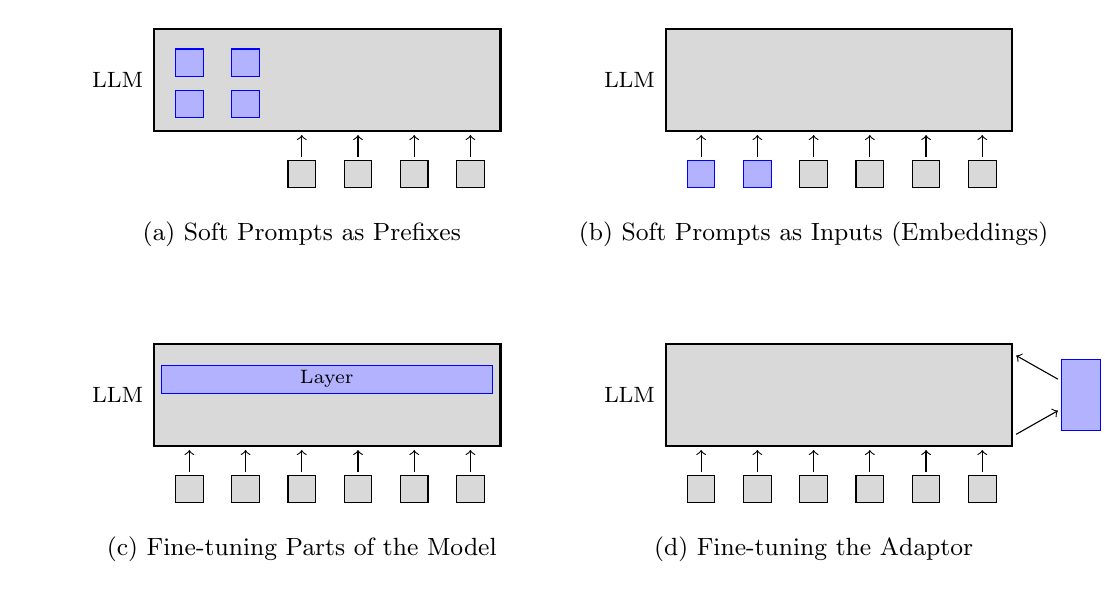
\begin{tikzpicture}
	
\def\ssep{0.35cm}
\def\bsep{2.0cm}

\tikzstyle{enode} = [minimum width=0.35cm,minimum height=0.35cm,inner sep=2pt,draw];
\tikzstyle{tnode} = [minimum width=4.4cm,minimum height=1.3cm,inner sep=2pt,draw,thick,fill=gray!30];

% prefix fine-tuning
\begin{scope}

\node [enode,anchor=west,draw=white] (e0) at (0,0) {};
\node [enode,anchor=west,draw=white] (e1) at ([xshift=\ssep]e0.east) {};
\node [enode,anchor=west,fill=gray!30] (e2) at ([xshift=\ssep]e1.east) {};
\node [enode,anchor=west,fill=gray!30] (e3) at ([xshift=\ssep]e2.east) {};
\node [enode,anchor=west,fill=gray!30] (e4) at ([xshift=\ssep]e3.east) {};
\node [enode,anchor=west,fill=gray!30] (e5) at ([xshift=\ssep]e4.east) {};

\node [tnode,anchor=south west] (model) at ([yshift=\ssep,xshift=-0.8*\ssep]e0.north west) {};
\node [anchor=east] (modellabel) at ([xshift=0pt]model.west) {\footnotesize{LLM}};

\draw [->,white] ([yshift=1pt]e0.north) -- ([yshift=\ssep-1pt]e0.north);
\draw [->,white] ([yshift=1pt]e1.north) -- ([yshift=\ssep-1pt]e1.north);
\draw [->] ([yshift=1pt]e2.north) -- ([yshift=\ssep-1pt]e2.north);
\draw [->] ([yshift=1pt]e3.north) -- ([yshift=\ssep-1pt]e3.north);
\draw [->] ([yshift=1pt]e4.north) -- ([yshift=\ssep-1pt]e4.north);
\draw [->] ([yshift=1pt]e5.north) -- ([yshift=\ssep-1pt]e5.north);

\node [enode,anchor=south,draw=blue,fill=blue!30] (p0) at ([yshift=1.5*\ssep]e0.north) {};
\node [enode,anchor=south,draw=blue,fill=blue!30] (p1) at ([yshift=1.5*\ssep]e1.north) {};

\node [enode,anchor=south,draw=blue,fill=blue!30] (p01) at ([yshift=3.0*\ssep]e0.north) {};
\node [enode,anchor=south,draw=blue,fill=blue!30] (p11) at ([yshift=3.0*\ssep]e1.north) {};

\node [anchor=north] (caption) at ([yshift=-0.3cm]e2.south) {\small{(a) Soft Prompts as Prefixes}};

\end{scope}

% soft prompts as token embeddings
\begin{scope}[xshift=6.5cm]

\node [enode,anchor=west,draw=blue,fill=blue!30] (e0) at (0,0) {};
\node [enode,anchor=west,draw=blue,fill=blue!30] (e1) at ([xshift=\ssep]e0.east) {};
\node [enode,anchor=west,fill=gray!30] (e2) at ([xshift=\ssep]e1.east) {};
\node [enode,anchor=west,fill=gray!30] (e3) at ([xshift=\ssep]e2.east) {};
\node [enode,anchor=west,fill=gray!30] (e4) at ([xshift=\ssep]e3.east) {};
\node [enode,anchor=west,fill=gray!30] (e5) at ([xshift=\ssep]e4.east) {};

\node [tnode,anchor=south west] (model) at ([yshift=\ssep,xshift=-0.8*\ssep]e0.north west) {};
\node [anchor=east] (modellabel) at ([xshift=0pt]model.west) {\footnotesize{LLM}};

\draw [->] ([yshift=1pt]e0.north) -- ([yshift=\ssep-1pt]e0.north);
\draw [->] ([yshift=1pt]e1.north) -- ([yshift=\ssep-1pt]e1.north);
\draw [->] ([yshift=1pt]e2.north) -- ([yshift=\ssep-1pt]e2.north);
\draw [->] ([yshift=1pt]e3.north) -- ([yshift=\ssep-1pt]e3.north);
\draw [->] ([yshift=1pt]e4.north) -- ([yshift=\ssep-1pt]e4.north);
\draw [->] ([yshift=1pt]e5.north) -- ([yshift=\ssep-1pt]e5.north);

\node [anchor=north] (caption) at ([yshift=-0.3cm]e2.south) {\small{(b) Soft Prompts as Inputs (Embeddings)}};

\end{scope}

% fine-tuning parts of the model
\begin{scope}[yshift=-4cm]

\node [enode,anchor=west,fill=gray!30] (e0) at (0,0) {};
\node [enode,anchor=west,fill=gray!30] (e1) at ([xshift=\ssep]e0.east) {};
\node [enode,anchor=west,fill=gray!30] (e2) at ([xshift=\ssep]e1.east) {};
\node [enode,anchor=west,fill=gray!30] (e3) at ([xshift=\ssep]e2.east) {};
\node [enode,anchor=west,fill=gray!30] (e4) at ([xshift=\ssep]e3.east) {};
\node [enode,anchor=west,fill=gray!30] (e5) at ([xshift=\ssep]e4.east) {};

\node [tnode,anchor=south west] (model) at ([yshift=\ssep,xshift=-0.8*\ssep]e0.north west) {};
\node [anchor=east] (modellabel) at ([xshift=0pt]model.west) {\footnotesize{LLM}};

\draw [->] ([yshift=1pt]e0.north) -- ([yshift=\ssep-1pt]e0.north);
\draw [->] ([yshift=1pt]e1.north) -- ([yshift=\ssep-1pt]e1.north);
\draw [->] ([yshift=1pt]e2.north) -- ([yshift=\ssep-1pt]e2.north);
\draw [->] ([yshift=1pt]e3.north) -- ([yshift=\ssep-1pt]e3.north);
\draw [->] ([yshift=1pt]e4.north) -- ([yshift=\ssep-1pt]e4.north);
\draw [->] ([yshift=1pt]e5.north) -- ([yshift=\ssep-1pt]e5.north);

\node [anchor=west,minimum width=4.2cm,minimum height=0.3cm,fill=blue!30,draw=blue,inner sep=2pt] (layer) at ([xshift=0.1cm,yshift=0.2cm]model.west) {\scriptsize{Layer}};

\node [anchor=north] (caption) at ([yshift=-0.3cm]e2.south) {\small{(c) Fine-tuning Parts of the Model}};

\end{scope}

% fine-tuning an adaptor
\begin{scope}[yshift=-4cm,xshift=6.5cm]

\node [enode,anchor=west,fill=gray!30] (e0) at (0,0) {};
\node [enode,anchor=west,fill=gray!30] (e1) at ([xshift=\ssep]e0.east) {};
\node [enode,anchor=west,fill=gray!30] (e2) at ([xshift=\ssep]e1.east) {};
\node [enode,anchor=west,fill=gray!30] (e3) at ([xshift=\ssep]e2.east) {};
\node [enode,anchor=west,fill=gray!30] (e4) at ([xshift=\ssep]e3.east) {};
\node [enode,anchor=west,fill=gray!30] (e5) at ([xshift=\ssep]e4.east) {};

\node [tnode,anchor=south west] (model) at ([yshift=\ssep,xshift=-0.8*\ssep]e0.north west) {};
\node [anchor=east] (modellabel) at ([xshift=0pt]model.west) {\footnotesize{LLM}};

\draw [->] ([yshift=1pt]e0.north) -- ([yshift=\ssep-1pt]e0.north);
\draw [->] ([yshift=1pt]e1.north) -- ([yshift=\ssep-1pt]e1.north);
\draw [->] ([yshift=1pt]e2.north) -- ([yshift=\ssep-1pt]e2.north);
\draw [->] ([yshift=1pt]e3.north) -- ([yshift=\ssep-1pt]e3.north);
\draw [->] ([yshift=1pt]e4.north) -- ([yshift=\ssep-1pt]e4.north);
\draw [->] ([yshift=1pt]e5.north) -- ([yshift=\ssep-1pt]e5.north);

\node [anchor=west,minimum width=0.5cm,minimum height=0.9cm,fill=blue!30,draw=blue] (adaptor) at ([xshift=0.6cm]model.east) {};
\node [anchor=west,rotate=90] (adaptorlabel) at ([xshift=0.2cm,yshift=-0.5cm]adaptor.east) {\tiny{Adaptor}};
\draw [<-] ([xshift=-1pt,yshift=-0.2cm]adaptor.west) -- ([xshift=1pt,yshift=-0.5cm]model.east);
\draw [->] ([xshift=-1pt,yshift=0.2cm]adaptor.west) -- ([xshift=1pt,yshift=0.5cm]model.east);

\node [anchor=north] (caption) at ([yshift=-0.3cm]e2.south) {\small{(d) Fine-tuning the Adaptor}};

\end{scope}

\end{tikzpicture}
\end{center}

\caption{Illustrations of using soft prompts in LLMs. Here tunable soft prompts are shown in blue, and components whose parameters are fixed during fine-tuning are shown in gray. In sub-figure (a), soft prompts are prefixes appended to each layer of the LLM. In sub-figure (b), soft prompts are used as input embeddings for the LLM. In sub-figures (c) and (d), soft prompts are broadly treated as components of the model that are fine-tuned for task adaptation.}
\label{fig:comparison-of-soft-prompts-in-llms}
\end{figure}

\subsubsection{Learning Soft Prompts with Compression}

\noindent Another approach to learning soft prompts is to frame it as a compression problem. As a simple example, consider the problem of approximating a long context using a continuous representation~\cite{wingate-etal:2022prompt}. Suppose we have a user input $\mathbf{z}$ and its context $\mathbf{c}$ (such as long instructions and demonstrations). Now we want to learn a compressed representation of the context, denoted by $\sigma$, such that the prediction conditioned on $\mathbf{z}$ and $\sigma$
is as close as possible to that conditioned on $\mathbf{z}$ and $\mathbf{c}$. This goal can be loosely formulated as
\begin{eqnarray}
\hat{\sigma} & = & \argmin_{\sigma} s(\hat{\mathbf{y}},\hat{\mathbf{y}}_{\sigma}),
\end{eqnarray}

\noindent where $\hat{\mathbf{y}} = \argmax_{\mathbf{y}} \Pr(\mathbf{y}|\mathbf{c},\mathbf{z})$ and $\hat{\mathbf{y}}_{\sigma} = \argmax_{\mathbf{y}} \Pr(\mathbf{y}|\sigma,\mathbf{z})$ are the LLM predictions given the full context and the compressed context, respectively. The function $s(\cdot,\cdot)$ measures the discrepancy between the two predictions.

One general framework for achieving this is knowledge distillation, where $\hat{\mathbf{y}}$ and $\hat{\mathbf{y}}_{\sigma}$ can be seen as the predictions of the teacher model and the student model, respectively. This formalization links our discussion to the context distillation problem discussed earlier. The training objective can be defined analogously to Eqs.~(\ref{eq:context-distillation-simple}) and~(\ref{eq:context-distillation-kl}). For instance, a straightforward maximum likelihood objective is given by
\begin{eqnarray}
\hat{\sigma} & = & \argmax_{\sigma} \log \Pr(\hat{\mathbf{y}}|\sigma, \mathbf{z}).
\end{eqnarray}

\noindent Alternatively, we can minimize the KL divergence between the output distributions, giving
\begin{eqnarray}
\hat{\sigma} & = & \argmin_{\sigma} \mathrm{D}_{\mathrm{KL}}(\Pr(\cdot|\mathbf{c},\mathbf{z}) \,\|\, \Pr(\cdot|\sigma,\mathbf{z})).
\end{eqnarray}

\noindent The difference with the models in Eqs.~(\ref{eq:context-distillation-simple}) and~(\ref{eq:context-distillation-kl}) is that here the compressed context is represented as real-valued vectors (call them \mindex{prompt embeddings}), rather than as normal tokens. By applying the above methods, we distill the context from the token sequence $\mathbf{c}$ into the embeddings $\sigma$. Note that the teacher model $\Pr(\cdot|\mathbf{c},\mathbf{z})$ and the student model $\Pr(\cdot|\sigma,\mathbf{z})$ may not share the same architecture or model settings. In practice, we generally wish for the teacher model to be stronger, while the student model should be smaller and more efficient.

While compressing full context into continuous representations is a straightforward approach to learning soft prompts, it requires a teacher model that can deal with long input sequences. In many cases, however, the context is so long that applying an LLM is too costly or infeasible. Modeling long input sequences can fall under the broad family of efficient methods for long-context LLMs. Many techniques have been developed to address this issue. For example, one can use a fixed-size KV cache to store the past information at each step during inference. Efficient Transformer architectures and long-context LLMs have been extensively discussed in this book. For more detailed discussions of these topics, interested readers can refer to Chapter \ChapterLLM.

There are also methods specifically designed to compress long sequences into soft prompts. Here we consider \citet{chevalier-etal:2023adapting}'s method as an example. The basic idea is to gradually learn soft prompts by compressing the input sequence into a fixed-size representation. For simplicity, we use $\mathbf z$ to denote the entire input sequence to be compressed. Given a long input sequence, we first divide it into a number of segments $\{\mathbf{z}^1, \cdots, \mathbf{z}^K\}$. We then process these segments in sequence, each time generating a representation of the input we have processed so far, denoted by $\sigma^{<i+1}$. To do this, a few summary tokens ${\langle \mathrm{g}_1 \rangle, \cdots, \langle \mathrm{g}_{\kappa} \rangle}$ are introduced. At each step, we take a segment $\mathbf{z}^i = z_1^{i} \cdots z_{m_i}^{i}$, along with the previous compressed representation $\sigma^{<i}$ and the summary tokens $\langle \mathrm{g}_1 \rangle, \cdots, \langle \mathrm{g}_{\kappa} \rangle$ as input, and use an LLM to produce the corresponding hidden representation sequence at the last Transformer layer. An example of this process is illustrated in Figure~\ref{fig:compressing-context-with-summary-tokens}.

\begin{figure}[!t]
\centering
% !Mode:: "TeX:UTF-8"
% !TEX encoding = UTF-8 Unicode

\begin{center}
\begin{tikzpicture}
	
\def\ssep{0.3cm}
\def\bsep{2.0cm}

\tikzstyle{enode} = [minimum width=0.8cm,minimum height=0.8cm,inner sep=2pt];
\tikzstyle{lnode} = [minimum width=9.2cm,minimum height=1.3cm,inner sep=2pt];

\begin{scope}

\node [enode,anchor=center,fill=red!20] (e1) at (0,0) {\footnotesize{$\sigma^{<i}_1$}};
\node [enode,anchor=west,fill=red!20] (e2) at ([xshift=\ssep]e1.east) {\footnotesize{$\sigma^{<i}_2$}};
\node [enode,anchor=west,fill=ugreen!20] (e3) at ([xshift=\ssep]e2.east) {\footnotesize{$\mathbf{e}_1^i$}};
\node [enode,anchor=west,fill=ugreen!20] (e4) at ([xshift=\ssep]e3.east) {\footnotesize{$\mathbf{e}_2^i$}};
\node [enode,anchor=west,fill=ugreen!20] (e5) at ([xshift=\ssep]e4.east) {\footnotesize{$\mathbf{e}_3^i$}};
\node [enode,anchor=west,fill=ugreen!20] (e6) at ([xshift=\ssep]e5.east) {\footnotesize{$\mathbf{e}_4^i$}};
\node [enode,anchor=west,fill=blue!20,inner sep=0pt] (e7) at ([xshift=\ssep]e6.east) {\footnotesize{$\langle \mathbf{e}_1 \rangle$}};
\node [enode,anchor=west,fill=blue!20,inner sep=0pt] (e8) at ([xshift=\ssep]e7.east) {\footnotesize{$\langle \mathbf{e}_2 \rangle$}};

\node [enode,anchor=north] (x3) at ([yshift=-0.3cm]e3.south) {\footnotesize{$z_1^i$}};
\node [enode,anchor=north] (x4) at ([yshift=-0.3cm]e4.south) {\footnotesize{$z_2^i$}};
\node [enode,anchor=north] (x5) at ([yshift=-0.3cm]e5.south) {\footnotesize{$z_3^i$}};
\node [enode,anchor=north] (x6) at ([yshift=-0.3cm]e6.south) {\footnotesize{$z_4^i$}};
\node [enode,anchor=north] (x7) at ([yshift=-0.3cm]e7.south) {\footnotesize{$\langle \mathrm{g}_1 \rangle$}};
\node [enode,anchor=north] (x8) at ([yshift=-0.3cm]e8.south) {\footnotesize{$\langle \mathrm{g}_2 \rangle$}};

\draw [->] ([yshift=-3pt]x3.north) -- ([yshift=-1pt]e3.south);
\draw [->] ([yshift=-3pt]x4.north) -- ([yshift=-1pt]e4.south);
\draw [->] ([yshift=-3pt]x5.north) -- ([yshift=-1pt]e5.south);
\draw [->] ([yshift=-3pt]x6.north) -- ([yshift=-1pt]e6.south);
\draw [->] ([yshift=-3pt]x7.north) -- ([yshift=-1pt]e7.south);
\draw [->] ([yshift=-3pt]x8.north) -- ([yshift=-1pt]e8.south);

\node [lnode,anchor=south west,draw,thick] (transformer) at ([xshift=-0.3cm,yshift=0.4cm]e1.north west) {};
\node [anchor=south] (tcaption) at ([yshift=0.3cm]transformer.south) {\Large{Transformer Layers}};

\node [enode,anchor=south,fill=gray!30] (h1) at ([yshift=2.2cm]e1.north) {\footnotesize{\color{black!30} $\mathbf{h}^{<i}_1$}};
\node [enode,anchor=south,fill=gray!30] (h2) at ([yshift=2.2cm]e2.north) {\footnotesize{\color{black!30} $\mathbf{h}^{<i}_1$}};
\node [enode,anchor=south,fill=gray!30] (h3) at ([yshift=2.2cm]e3.north) {\footnotesize{\color{black!30} $\mathbf{h}_1$}};
\node [enode,anchor=south,fill=gray!30] (h4) at ([yshift=2.2cm]e4.north) {\footnotesize{\color{black!30} $\mathbf{h}_2$}};
\node [enode,anchor=south,fill=gray!30] (h5) at ([yshift=2.2cm]e5.north) {\footnotesize{\color{black!30} $\mathbf{h}_3$}};
\node [enode,anchor=south,fill=gray!30] (h6) at ([yshift=2.2cm]e6.north) {\footnotesize{\color{black!30} $\mathbf{h}_4$}};
\node [enode,anchor=south,fill=red!20,inner sep=0pt] (h7) at ([yshift=2.2cm]e7.north) {\tiny{$\sigma^{<i+1}_1$}};
\node [enode,anchor=south,fill=red!20,inner sep=0pt] (h8) at ([yshift=2.2cm]e8.north) {\tiny{$\sigma^{<i+1}_2$}};

\draw [->] ([yshift=1pt]e1.north) -- ([yshift=0.37cm]e1.north);
\draw [->] ([yshift=1pt]e2.north) -- ([yshift=0.37cm]e2.north);
\draw [->] ([yshift=1pt]e3.north) -- ([yshift=0.37cm]e3.north);
\draw [->] ([yshift=1pt]e4.north) -- ([yshift=0.37cm]e4.north);
\draw [->] ([yshift=1pt]e5.north) -- ([yshift=0.37cm]e5.north);
\draw [->] ([yshift=1pt]e6.north) -- ([yshift=0.37cm]e6.north);
\draw [->] ([yshift=1pt]e7.north) -- ([yshift=0.37cm]e7.north);
\draw [->] ([yshift=1pt]e8.north) -- ([yshift=0.37cm]e8.north);

\draw [<-,gray] ([yshift=-1pt]h1.south) -- ([yshift=-0.4cm]h1.south);
\draw [<-,gray] ([yshift=-1pt]h2.south) -- ([yshift=-0.4cm]h2.south);
\draw [<-,gray] ([yshift=-1pt]h3.south) -- ([yshift=-0.4cm]h3.south);
\draw [<-,gray] ([yshift=-1pt]h4.south) -- ([yshift=-0.4cm]h4.south);
\draw [<-,gray] ([yshift=-1pt]h5.south) -- ([yshift=-0.4cm]h5.south);
\draw [<-,gray] ([yshift=-1pt]h6.south) -- ([yshift=-0.4cm]h6.south);
\draw [<-] ([yshift=-1pt]h7.south) -- ([yshift=-0.4cm]h7.south);
\draw [<-] ([yshift=-1pt]h8.south) -- ([yshift=-0.4cm]h8.south);

\begin{pgfonlayer}{background}
\node [draw,dotted,thick] [fit = (e1) (e2)] (softlast) {};
\node [draw,dotted,thick] [fit = (h7) (h8)] (softcur) {};
\end{pgfonlayer}

\node [anchor=east] (softlastl) at ([xshift=-0.1cm]softlast.west) {\footnotesize{Soft Prompts}};
\node [anchor=north west] (softlast2) at ([yshift=0.2cm]softlastl.south west) {\footnotesize{at Step $i-1$}};

\node [anchor=west] (softcurl) at ([xshift=0.1cm]softcur.east) {\footnotesize{Soft Prompts}};
\node [anchor=north west] (softcur2) at ([yshift=0.2cm]softcurl.south west) {\footnotesize{at the Current Step}};

\end{scope}

\end{tikzpicture}
\end{center}

\caption{Illustration of compressing a context segment into soft prompts ($\kappa = 2$ and $m_i = 4$). The input to the LLM includes the soft prompts from the previous step ($\sigma^{<i}_1$ and $\sigma^{<i}_2$), the tokens of the segment ($z_1, z_2, z_3,$ and $z_4$), and the summary tokens ($\langle \mathrm{g}_1 \rangle$ and $\langle \mathrm{g}_2 \rangle$). Given these, the LLM operates as usual. We then extract the outputs at the last Transformer layer that correspond to the summary tokens. These outputs can be viewed as the soft prompts that accumulated up to this segment.}
\label{fig:compressing-context-with-summary-tokens}
\end{figure}

Here $\sigma^{<i}$ is essentially a memory. The model operates in an RNN fashion. Each time we take a segment and update this memory by encoding both the previous memory state and the segment. Therefore, the $\sigma^{<i}$ produced at the last segment is a representation of the entire context sequence. The Transformer model for learning these representations can be a standard LLM but we need to fine-tune it to adapt to this context representation task.

Note that here we simply consider \textit{prompt} and \textit{context} as similar terms, even though they are not the same. Although we use the term \textit{prompt} broadly to include contextual information supplied to the model., we can often view it as a type of context. From this perspective, the methods discussed here can be applied to general text compression problems.

\subsection{Prompt Length Reduction}

While soft prompts provide dense hidden representations, they are generally not directly interpretable. This lack of interpretability makes it difficult for users to understand how prompts influence LLM outputs. Moreover, modifying soft prompts often requires additional fine-tuning, which limits their utility in dynamic environments where prompts frequently change.

One alternative approach to improving prompt efficiency is to simplify the prompt text itself. Unlike soft prompts, simplified textual prompts remain interpretable and can be modified directly by users. For example, below is a prompt for answering questions on healthcare and finance.

\vspace{0.5em}
\begin{tcolorbox}[frame empty]

\begingroup
\setlength{\leftskip}{2em}
\setlength{\rightskip}{2em}

The task involves developing a language model capable of understanding and responding to user inquiries across various domains, with a particular emphasis on healthcare and finance. Considering the broad range of potential queries, from the specifics of medical diagnoses to the nuances of financial regulations, the model must ensure a comprehensive understanding and accurate responses.

\vspace{0.5em}

Question:

\vspace{0.2em}

What are the best practices for using artificial intelligence in diagnosing cardiovascular diseases?

\vspace{0.5em}

\underline{\hspace{2em}}

\endgroup

\end{tcolorbox}
\vspace{0.5em}

We can simplify the task description by deleting the unimportant parts.

\vspace{0.5em}

\begin{center}
\parbox{0.8\linewidth}{
\textit{The task involves developing a language model capable of understanding and responding to user inquiries {\color{gray} \sout{across various domains, with a particular emphasis}} on healthcare and finance. {\color{gray} \sout{Considering the broad range of potential queries, from the specifics of medical diagnoses to the nuances of financial regulations,}} The model must ensure a comprehensive understanding and accurate responses.}
}
\end{center}

\vspace{0.5em}

We can also paraphrase it into a shorter text.

\vspace{0.5em}

\begin{center}
\parbox{0.8\linewidth}{
\textit{The task involves developing a language model focused on healthcare and finance, capable of understanding and accurately responding to a wide range of user inquiries.}
}
\end{center}

\vspace{0.5em}

This problem can be viewed as a standard NLP task --- text simplification. Therefore, the methods used for text simplification are generally applicable and not limited to prompt simplification. There are many ways to achieve this. One simple method is to define some heuristics and identify redundant words that can be eliminated without losing essential information. For example, we can examine each token in a sequence in terms of its contribution to the overall meaning and remove those that provide minimal value~\cite{li-etal:2023compressing,jiang-etal:2023llmlingua}. Another method involves framing the problem as a sequence-to-sequence task. Given labeled data for text simplification, we can train an encoder-decoder model to transform each input text into its simplified form. In addition, given that many LLMs have been fine-tuned and aligned to perform text simplification tasks, it is straightforward to use these models to simplify prompts. For example, we can prompt an LLM to simplify a prompt while satisfying constraints such as length limits.

%----------------------------------------------------------------------------------------
% NEW SECTION
%----------------------------------------------------------------------------------------

\section{Summary}

\noindent In this chapter, we have discussed a variety of topics related to LLM prompting. Our discussion has focused mainly on two aspects:

\begin{itemize}
\item \vspace{0.5em} How to design basic prompts to guide the predictions of LLMs and refine these prompts for more effective and efficient problem-solving?
\item \vspace{0.3em} How to automate the design and representation of prompts?
\end{itemize}
\vspace{0.3cm}

\noindent Solutions to these issues involve both general prompt designs and more advanced techniques, such as CoT and prompt learning, which have been explored extensively in recent research.

In NLP, prompting can be viewed as a technology that has evolved along with LLMs, and in a sense, it has opened the door to the practical application of these models in an impressive range of problem domains. In fact, if we expand the concept of prompts to some extent, it can be traced back to the early days of machine learning and NLP. For example, many NLP systems use hand-crafted features and templates to ``prompt'' specific tasks. Imagine developing a feature to indicate whether a text is formal or informal. We can feed this feature into a machine translation system to condition the translation on the type of the input text.

The widespread use of the modern concept of prompts began with the rise of large pre-trained models in the field of NLP. Initially, these models, such as BERT, were adapted to specific downstream tasks mainly through fine-tuning. However, researchers soon discovered that by designing specific ``prompts'' --- adding certain words or sentences to the input --- the models could be triggered to respond to specific tasks without extensive fine-tuning. This motivated the NLP community to develop and apply universal foundation models that can be prompted to address various tasks without changing the underlying architecture and the pre-training procedure.

Prompting approaches were first experimented with smaller models and later demonstrated impressive capabilities with large models like GPT-3, which could generate high-quality text in response to simple prompts across various tasks. As prompting technology evolved, prompt engineering emerged as a critical area of research. As discussed in this chapter, it broadly involves designing effective prompts to maximize model performance, encompassing both hand-crafted and automatically generated prompts. More recent research has explored how to enhance the effectiveness of prompting through techniques like few-shot learning, zero-shot learning, and CoT reasoning, enabling LLMs to work effectively across a wide range of scenarios. A general discussion of prompting can be very broad, and we cannot cover all details in this chapter. For more advanced techniques of prompting, the reader can refer to recent surveys. Topics include in-context learning~\cite{li:2023practical,dong-etal:2022survey}, CoT~\cite{chu-etal:2023survey,yu-etal:2023towards,zhang-etal:2023igniting}, efficient prompting~\cite{chang-etal:2024efficient}, and general prompt engineering~\cite{liu2023-etal:prompting,chen-etal:2023unleashing}.

Note that although we would ideally like to develop general prompting methods without adjusting model architectures and parameters, the results of prompting generally depend heavily on the quality and size of the given LLMs. For stronger models, such as commercialized online LLMs, simple prompts may be sufficient to instruct these models to perform tasks correctly. In this case, prompt engineering is relatively easy, though careful prompt refinement remains necessary. By contrast, for less capable or smaller-scale models, we may need to carefully design the prompts to achieve the desired results. In many cases, fine-tuning is still necessary to adapt the models to sophisticated prompting strategies.

